%!TEX TS-program = pdflatex
% dissertation.tex -- main dissertation file
%
% Wisconsin dissertation template
% Copyright (c) 2008-2009 William C. Benton.  All rights reserved.
%
% This program can redistributed and/or modified under the terms
% of the LaTeX Project Public License Distributed from CTAN
% archives in directory macros/latex/base/lppl.txt; either
% version 1 of the License, or (at your option) any later version.
%
% This program includes other software that is licensed under the
% terms of the LPPL and the Perl Artistic License; see README for details.
%
% You, the user, still hold the copyright to any document you produce
% with this software (like your dissertation).
%

%%% You'll want ``oneside'' for the deposit version, but probably not for any versions that don't need to meet the UW requirements
\documentclass[11pt,oneside,letterpaper,oldfontcommands]{memoir}

\usepackage{alltt}
\usepackage{amsfonts} 
\usepackage{amsmath}
\usepackage{array}
\usepackage{balance}
\usepackage{bigstrut}
\usepackage{booktabs}
\usepackage{boxedminipage}
\usepackage{colortbl}
\usepackage{fixltx2e}
\usepackage{graphicx}
\usepackage{multirow}
\usepackage{nicefrac}
\usepackage{pdflscape}
\usepackage{pifont}
\usepackage{setspace}
\usepackage{subfig}
\usepackage{xcolor}
\usepackage{xspace}

\setsecnumdepth{subsubsection}

\input{includes/preamble}
\input{includes/defs}
\input{includes/thesisdefs}
\svnidlong{$LastChangedBy$}{$LastChangedRevision$}{$LastChangedDate$}{$HeadURL: http://freevariable.com/dissertation/branches/diss-template/dissertation.tex $} 


\newenvironment{ParaEnum}[0]{\begin{inparaenum}[(1)]}{\end{inparaenum}}


\newcommand{\TextArrow}[3]{\tikz[#1]{\draw[->, #2] (0, 0) to[#3] (.5, 0) {} ;}}
\newcommand{\StraightSolidArrow}[0]{\TextArrow{baseline=-2pt}{}{}}
\newcommand{\CrashArrow}[0]{\StraightSolidArrow}
\newcommand{\CorruptArrow}[0]{\TextArrow{}{densely dotted}{bend right}}

\newcommand{\TwoRowHeader}[2]{\multirow{-2}{*}{\setlength{\tabcolsep}{0pt}\begin{tabular}{r}#1\\#2\end{tabular}}}
\newcommand{\nocaptionrule}{%
  \@setflag \@caprule = \@false}

\newcommand{\YesRank}[1]{\checkmark{} $#1$}
%\newcommand{\Yes}[0]{\checkmark}
%\newcommand{\No}[0]{-}
\newcommand{\Code}[1]{\lstinline{#1}}




\newsavebox{\Plus}
\newsavebox{\Minus}
\savebox{\Plus}{\scriptsize\textsf{+}}
\savebox{\Minus}{\scriptsize\textsf{\textminus}}

\renewcommand{\cite}[1]{%
  \PackageError{natbib}{%
    The \string\cite\space{} command is ambiguous; use
    \string\citet\space{} or \string\citep\space{} instead}{}}

\renewcommand{\autoref}[1]{%
  \PackageError{cleveref}{%
    Do not use \string\autoref.  Use \string\cref instead, or use
    \string\crefrange for ranges of referenced items}}

\renewcommand{\hline}[1]{%
  \PackageError{booktabs}{%
    Do not use \string\hline.  Use \string\toprule, \string\midrule,
    or \string\bottomrule\space instead depending on where in the
    table the line appears}}


\crefname{figure}{Figure}{Figures}
\crefname{section}{Section}{Sections}
\crefname{chapter}{Chapter}{Chapters}
\crefname{table}{Table}{Tables}
\crefname{guideline}{guideline}{guidelines}

\setcitestyle{comma,numbers,sort&compress,square}

\hyphenation{Lite-Race}

\widowpenalty10000
\clubpenalty10000

\lstdefinelanguage{example}{%
  morekeywords={lock,unlock,reentrant_lock,reentrant_unlock},
}

\lstset{%
  basicstyle=\sffamily,
  columns=fullflexible,
  showstringspaces=false,
  upquote=true,
  literate={"}{\textquotedbl}1,
  language=C++,
  escapeinside={/*@}{@*/},
  mathescape,
  numbersep=1ex,
  keepspaces=true,
}

\usetikzlibrary{calc}
\usetikzlibrary{chains}
\usetikzlibrary{matrix}
\usetikzlibrary{positioning}
\usetikzlibrary{shapes}

\tikzset{%
  node distance=1em,
  >=stealth,
  cfg/.style={%
    minimum width=1em,
    minimum height=1em,
    rounded corners=2pt,
    draw=black,
  },
  protected/.style={%
    cfg,
    fill=black!20,
  },
  ghost/.style={%
    minimum width=0,
    minimum height=0,
    shape=coordinate,
  },
  mutex/.style={%
    midway,
    sloped,
  },
  interleaving/.style={%
    matrix,
    matrix of nodes,
    column sep=4em,
    row sep=2em,
  },
}

\newcommand{\SignalSymbol}[0]{\Lightning}
\DeclareRobustCommand\SignalText{\tikz \node [rotate=-90, inner sep=1pt] {\large\SignalSymbol} ;}
\newcommand{\Signal}[0]{\contour{white}{\LARGE\SignalSymbol}}

\newcommand{\code}[1]{\texttt{#1}}
\newcommand{\codefamily}[0]{\sffamily}

\newcommand{\allbugs}{110\xspace}
\newcommand{\heavybugs}{66\xspace}


\newcommand{\codefig}[1]{%
  \centering
  \framebox{\lstinputlisting[boxpos=t\footnotesize]{figures/#1.c}}}

\newcommand{\Tool}{LDoctor\xspace}



\clearpage\pagenumbering{roman}  % This makes the page numbers Roman (i, ii, etc)

\title{Understanding, Detecting and Diagnosing Real-World Performance Bugs}
\author{Linhai Song}
\department{Computer Sciences}

\date{2015}

\begin{document}

%%% Uncomment the following if your .bib contains references that you will not 
%%% explicitly cite, but that should be in the final bibliography:
% \nocite{*}

\ifpdf
\DeclareGraphicsExtensions{.pdf, .jpg, .tif}
\else
\DeclareGraphicsExtensions{.eps, .jpg}
\fi

\maketitle

%% Add \part declarations if you want, but it's not necessary
%\part{Preliminaries}

\svnidlong{$LastChangedBy$}{$LastChangedRevision$}{$LastChangedDate$}{$HeadURL: http://freevariable.com/dissertation/branches/diss-template/frontmatter/frontmatter.tex $}
\vcinfo{}

%%% SOME OF THIS CODE IS ADAPTED FROM THE VENERABLE withesis.cls

% COPYRIGHT PAGE
%  - To include a copyright page use \copyrightpage
\copyrightpage

% DEDICATION
\begin{dedication}
	\emph{To my parents, Zuoyu Song and Cuihua Fu.}
\end{dedication}

%% BEGIN PAGESTYLE

%%% You can pick a pagestyle if you want; see the memoir class
%%% documentation for more info.  The default ``deposit'' option meets
%%% the UW thesis typesetting requirements but is probably
%%% unsatisfactory for making a version of your dissertation that
%%% won't be deposited to the graduate school (e.g. for web or a nice
%%% printed copy)

\chapterstyle{deposit}
\pagestyle{deposit}


% ACKNOWLEDGMENTS
\begin{acks}
First and foremost, I would like to express my wholehearted gratitude to my advisor, 
Professor Shan Lu, for her generous support and guidance during my PhD. 

The first email I sent to Shan is to ask whether I could provide her name as my potential advisor, when I applied my student visa. 
Shan kindly approved this. 
I am so lucky to begin my independent study with her immediately after I came to US. 
I can still remember the joy in my heart when she told me that she would pick me as her student, after we submit AFix. 

Throughout my PhD, Shan gave me numerous invaluable academic advice, 
ranging from the details of how to present data in my paper to the broad vision of 
how to explore an initial research idea. 
Besides research, 
Shan also teaches me how to better communicate with other people, 
how to manage my time, and how to be confident. 
Shan served as my role model in the past five years. 
I am so fortunate to observe and learn how she learns new knowledge, 
conducts research and succeeds in her career. 
PhD journey is tough. 
I feel extremely thankful for Shan's patience, support and actionable suggestions in each stage. 
I do not think I can get to the destination without her encouragement. 
 
I gratefully thank Professor Ben Liblit and Professor Darko Marinov for their kindly help during and after collaborating. 
Ben and Darko are always encouraging and helpful whenever I encounter research problems. 
Ben also helps me go through all paperwork and payment after Shan left to UChicago. 
I worked in Illinois for around one week, and it is an exciting experience to learn technical skills closely from Darko. 

I would like to thank all other committee members, Professor Remzi Arpaci-Dusseau, 
Professor Aws Albarghouthi, and Professor Xinyu Zhang, for their priceless comments and constructive criticisms on my thesis. 
It is really my honor to have all these professors on my committee. 
I would also thank Professor Loris D'Antoni for coming to my defense and leaving invaluable feedback. 

Thanks also go to every student in Shan's group and fellow students I worked with for 
the opportunity to learn together. 
I worked with Guoliang Jin on my first two research projects, and I want to thank him for helping me through my junior years. 
I want to thank Adrian Nistor for treating me so many lunches and solving so many weird problems I encountered in Illinois.
I want to thank Wei Zhang, Po-Chun Chang, Xiaoming Shi, Dongdong Deng, Rui Gu, Joy Arulraj, 
Joel Sherpelz, Haopeng Liu, and Yuxi Chen for making our group fun and exciting. 

I also want to thank many other people in UWisconsin. 
Thanks to Professor David Page, Professor Michael Swift, Professor Susan Horwitz, 
Professor Jerry Zhu, and Professor Eric Bach for knowledge I learned from their courses. 
Thanks to Angela Thorp for helping me through various administration stuff. 
Thanks to Peter Ohmann for suggestions about how to polish my talk. 
Thanks to my great roommates, Hao Wang, Ce Zhang, Jia Xu, and Huan Wang for giving me such great accompany. 
Thanks to all other good friends, Lanyue Lu, Wenfei Wu, Suli Yang, Yupu Zhang, Yiying Zhang, 
Jie Liu, Wentao Wu, Wenbin Fang, Weiyan Wang, Xiaozhu Meng, Junming Xu, Yimin Tan, Yizheng Chen, Ji Liu, Jun He, and Ao Ma for their help and support in different ways. 

I benefit a lot from my summer intern in NEC Labs America. 
I want to thank the company as well as my mentor Dr. Min Feng, for providing a terrific internship experience. 
 
Last but not least, I want to thank my parents back in China for their unconditional love and trust. 
Whenever I struggle with my PhD life, my parents are always supportive and encouraging. 
My work would not be nearly as meaningful without them. 
No words can express my gratitude and love to them. 
I dedicate the whole thesis to the most important persons in my life.  

\end{acks}

% CONTENTS, TABLES, FIGURES
\renewcommand{\printtoctitle}[1]{\chapter*{#1}}
\renewcommand{\printloftitle}[1]{\chapter*{#1}}
\renewcommand{\printlottitle}[1]{\chapter*{#1}}

\renewcommand{\tocmark}{}
\renewcommand{\lofmark}{}
\renewcommand{\lotmark}{}

\renewcommand{\tocheadstart}{}
\renewcommand{\lofheadstart}{}
\renewcommand{\lotheadstart}{}

\renewcommand{\aftertoctitle}{}
\renewcommand{\afterloftitle}{}
\renewcommand{\afterlottitle}{}

\renewcommand{\cftchapterfont}{\normalfont} 
\renewcommand{\cftsectionfont}{\itshape} 
\renewcommand{\cftchapterpagefont}{\normalfont} 
\renewcommand{\cftchapterpresnum}{\bfseries} 
\renewcommand{\cftchapterleader}{\hskip2mm} 
\renewcommand{\cftsectionleader}{\hskip2mm} 
\renewcommand{\cftchapterafterpnum}{\cftparfillskip} 
\renewcommand{\cftsectionafterpnum}{\cftparfillskip} 

% \captionnamefont{\small\sffamily} 
% \captiontitlefont{\small\sffamily} 

% \renewcommand{\contentsname}{contents}
% \renewcommand{\listfigurename}{list of figures}
% \renewcommand{\listtablename}{list of tables}

\tableofcontents

\clearpage
\listoftables

\clearpage
\listoffigures

%\clearpage
% NOMENCLATURE
 %\begin{conventions}
 %\begin{description}
 % \item{\makebox[0.75in][l]{term}
 %        \parbox[t]{5in}{definition\\}}
 % \end{description}
 %\input{frontmatter/conventions}
 %\end{conventions}

%\advisorname{Gottlob Frege}
%\advisortitle{Professor}
% ABSTRACT
%\begin{umiabstract}
%  Everyone wants software to run fast. 
Slow and inefficient software can easily frustrate end users and cause economic loss. 
Software-inefficiency problem has already caused several highly publicized failures. 
One major source of software's slowness is performance bug.
Performance bugs are software implementation mistakes that can cause inefficient execution. 
Performance bugs cannot be optimized away  by state-of-practice compilers. 
Many of them escape from in-house testing and manifest in front of end users, 
causing severe performance degradation and huge energy waste in the field. 
Performance bugs are becoming more critical, 
with the increasing complexity of modern software and workload,
the meager increases of single-core hardware performance, and the 
pressing energy concerns.
It is urgent to combat performance bugs.

This thesis works on three directions to fight performance bugs: 
performance bug understanding, rule-based performance-bug detection, 
and performance failure diagnosis. 

Building better tools needs a better understanding of performance bugs. 
In order to improve the understanding of performance bugs, 
we randomly sample 110 real-world performance bugs from 
5 large open-source software suites (Apache, Chrome, GCC, Mozilla and MySQL), 
and conduct the first empirical study on performance bugs. 
Our study is mainly performed to understand what are common root causes of performance bugs, 
how performance bugs are introduced, how to expose performance bugs and how to fix performance bugs. 
Important finds include: (1) there are dominating root causes and fix strategies for performance bugs, 
and root causes are highly correlated with fix strategies; 
(2) workload and API issues are two major reasons causing performance bugs to be introduced; 
(3) performance bugs require inputs with both special features and large scales to be exposed effectively. 
Our empirical study can guide future research on performance bugs, 
and it has already inspired our own performance-bug detection 
and performance failure diagnosis projects. 

Rule-based bug detection is widely used to detect functional bugs and security vulnerabilities. 
Inspired by our empirical study, we hypothesize that there are also statically 
checkable efficiency-related rules for performance bugs, 
violating which will lead to inefficient execution. 
These rules can be used to detect previously unknown performance bugs. 
To test our hypothesis, we manually examine fixed performance bugs, 
extract efficiency rules from performance bugs' patches, and implement static checkers to detect rules' violations. 
Our checkers find 332 previously unknown performance bugs. 
Some of found bugs have already been confirmed and fixed by developers. 
Our results demonstrate that rule-based performance-bug detection is a promising direction. 

Effectively diagnosing user-reported performance bugs is another key aspect of fighting performance bugs. 
Statistical debugging is one of the most effective failure diagnosis techniques designed for functional bugs. 
We explore the feasibility and design spaces to apply statistical debugging to performance failure diagnosis. 
We find that statistical debugging is a natural fit for diagnosing performance problems, 
which are often observed through comparison-based approaches and reported together 
with both good and bad inputs,
statistical debugging can effectively identify coarse-grained root causes 
for performance bugs under right types of design points, 
and special nature of performance bugs allows sampling to lower the 
overhead of runtime performance diagnosis without extending the diagnosis latency.

Performance bugs caused by inefficient loops contribute two thirds of user-reported performance bugs in our study. 
For them, coarse-grained root-cause information is not enough. 
To solve this problem, we first conduct an empirical study to understand what are fine-grained root
causes for inefficient loops in the real world. 
We then design LDoctor, which is a series of static-dynamic 
hybrid analysis routines that can help identify accurate fine-grained root-cause information. 
Sampling is leveraged to further lower diagnosis overhead, without hurting diagnosis accuracy or latency. 
Evaluation results show that LDoctor can cover most root-cause categories with good accuracy and small runtime overhead.

Our bug-detection technique and performance failure diagnosis techniques, 
guided by our empirical study, 
complement each other to significantly improve software performance. 

%\end{umiabstract}

\begin{nomenclature}
%\begin{description}

\begin{enumerate}

\item{{\textit{Performance bug:}}}
performance bugs are software implementation mistakes 
that can cause inefficient execution. 
We will use performance bugs
and performance problems interchangeably in this thesis 
following previous work in this 
area~\citep{Alabama,perf.fse10}.


\item{{\textit{Functional bug:}}}
functional bugs are software defects that lead to functional misbehavior, 
such as incorrect outputs, crashes, and hangs. 
Functional bugs include semantic bugs, 
memory bugs and concurrency bugs~\citep{LiASID06}.



\item{{\textit{Efficiency rule:}}}
efficiency rules are principles inside programs, 
violations of which will lead to inefficient execution. 
Efficiency rules usually contain two components, 
which indicate where and how a particular code transformation 
can be conducted to improve performance, 
while preserving original functionality. 


\item{{\textit{Root-cause information:}}}
for a particular failure, root-cause information includes a static code region causing the failure, 
explanation why the failure happens, and potential fix suggestions.


\item{{\textit{Inefficient loop:}}}
inefficient loops are loops that conduct inefficient computation due to performance bugs.

\item{{\textit{Diagnosis latency:}}}
diagnosis latency is the time it takes to figure out the root cause of a failure.                    
It is measured by
how many failure runs are needed in order to conduct failure diagnosis. 


\item{{\textit{Runtime overhead:}}}
runtime overhead is measured by comparing normal execution with monitored execution. 


%\item{\makebox[0.75in][l]{$V$}}    Voltage

%\item{\makebox[0.75in][l]{\$}}     US Dollars

\end{enumerate}
%\end{description}
\end{nomenclature}

%\clearpage
\begin{abstract}
  Everyone wants software to run fast. 
Slow and inefficient software can easily frustrate end users and cause economic loss. 
Software-inefficiency problem has already caused several highly publicized failures. 
One major source of software's slowness is performance bug.
Performance bugs are software implementation mistakes that can cause inefficient execution. 
Performance bugs cannot be optimized away  by state-of-practice compilers. 
Many of them escape from in-house testing and manifest in front of end users, 
causing severe performance degradation and huge energy waste in the field. 
Performance bugs are becoming more critical, 
with the increasing complexity of modern software and workload,
the meager increases of single-core hardware performance, and the 
pressing energy concerns.
It is urgent to combat performance bugs.

This thesis works on three directions to fight performance bugs: 
performance bug understanding, rule-based performance-bug detection, 
and performance failure diagnosis. 

Building better tools needs a better understanding of performance bugs. 
In order to improve the understanding of performance bugs, 
we randomly sample 110 real-world performance bugs from 
5 large open-source software suites (Apache, Chrome, GCC, Mozilla and MySQL), 
and conduct the first empirical study on performance bugs. 
Our study is mainly performed to understand what are common root causes of performance bugs, 
how performance bugs are introduced, how to expose performance bugs and how to fix performance bugs. 
Important finds include: (1) there are dominating root causes and fix strategies for performance bugs, 
and root causes are highly correlated with fix strategies; 
(2) workload and API issues are two major reasons causing performance bugs to be introduced; 
(3) performance bugs require inputs with both special features and large scales to be exposed effectively. 
Our empirical study can guide future research on performance bugs, 
and it has already inspired our own performance-bug detection 
and performance failure diagnosis projects. 

Rule-based bug detection is widely used to detect functional bugs and security vulnerabilities. 
Inspired by our empirical study, we hypothesize that there are also statically 
checkable efficiency-related rules for performance bugs, 
violating which will lead to inefficient execution. 
These rules can be used to detect previously unknown performance bugs. 
To test our hypothesis, we manually examine fixed performance bugs, 
extract efficiency rules from performance bugs' patches, and implement static checkers to detect rules' violations. 
Our checkers find 332 previously unknown performance bugs. 
Some of found bugs have already been confirmed and fixed by developers. 
Our results demonstrate that rule-based performance-bug detection is a promising direction. 

Effectively diagnosing user-reported performance bugs is another key aspect of fighting performance bugs. 
Statistical debugging is one of the most effective failure diagnosis techniques designed for functional bugs. 
We explore the feasibility and design spaces to apply statistical debugging to performance failure diagnosis. 
We find that statistical debugging is a natural fit for diagnosing performance problems, 
which are often observed through comparison-based approaches and reported together 
with both good and bad inputs,
statistical debugging can effectively identify coarse-grained root causes 
for performance bugs under right types of design points, 
and special nature of performance bugs allows sampling to lower the 
overhead of runtime performance diagnosis without extending the diagnosis latency.

Performance bugs caused by inefficient loops contribute two thirds of user-reported performance bugs in our study. 
For them, coarse-grained root-cause information is not enough. 
To solve this problem, we first conduct an empirical study to understand what are fine-grained root
causes for inefficient loops in the real world. 
We then design LDoctor, which is a series of static-dynamic 
hybrid analysis routines that can help identify accurate fine-grained root-cause information. 
Sampling is leveraged to further lower diagnosis overhead, without hurting diagnosis accuracy or latency. 
Evaluation results show that LDoctor can cover most root-cause categories with good accuracy and small runtime overhead.

Our bug-detection technique and performance failure diagnosis techniques, 
guided by our empirical study, 
complement each other to significantly improve software performance. 

\end{abstract}

\clearpage\pagenumbering{arabic}

%%% END STUFF TAKEN FROM WITHESIS EXAMPLE FILE


%% Now include the tex files for each chapter, like so (I put these in separate dirs): 
\chapter[Introduction]{Introduction}
\label{chap:introduction}
ToDo



\chapter[Background and Previous Work]{Background and Previous Work}
\label{chap:background}



\chapter[Real-World Performance-Bug Understanding]{Real-World Performance-Bug Understanding}
\label{chap:study}

Empirical studies on functional bugs have successfully guided the design of functional software testing, 
bug detection, and failure diagnosis. 
Poor understanding of performance bugs is part of the causes of today's performance-bug problems. 
The lack of empirical studies on performance bugs has severely 
limited the design of performance-bug avoidance, testing, detection, and fixing tools.

This chapter presents our comprehensive study of real-world performance bugs, 
based on 110 bugs randomly collected from the bug databases of five representative 
open-source software suites (Apache, Chrome, GCC, Mozilla, and MySQL). 
Following the lifetime of performance bugs, our empirical study is performed in 4 dimensions: 
the root-cause of performance bugs, how performance bugs are introduced, 
how to expose performance bugs and how to fix performance bugs. Our findings and implications can guide future research in this area, 
and have already inspired our own performance-bug detection and performance failure diagnosis work. 

\section{Introduction}
\label{sec:3_introduction}

Performance bugs~\citep{s2e,perf.fse10,rily.perftest,perfantipattern} 
are software implementation mistakes that can cause slow execution.
The patches for performance bugs are often not too complex.
These patches can preserve the same functionality, and achieve significant performance improvement. 
Performance bugs cannot be optimized away by compiler optimization. 
Many of them escape from testing process and manifest in front of end users~\citep{xiao13:context}.
Performance bugs are common and severe. 
Mozilla developers have to fix 5 to 50 performance bugs each month in the last 10 years. 
Performance bugs have already caused several highly publicized failures, 
like the slow affordable care act system~\citep{ACA-health}.
Fighting performance bugs is solely needed.  

There are many misunderstanding of performance bugs, 
such as ``performance is taken care of by compilers and hardware'' and 
``profiling is sufficient to solve performance problems''. 
These wrong perceptions are partly the causes of today's performance-bug problem~\citep{lies}. 
The lack of understanding of performance bugs has severely limited the research and tool building in this area. 

There are many empirical studies on functional bugs~\citep{chou01empirical,characteristics.asplos08, 10yearlinux,emmett.ppopp10,
sullivan92comparison,Lu.study.fast}. 
Many of them are conducted along the following dimensions: 
root causes of functional bugs, 
how functional bugs are introduced, how to expose functional bugs, 
and how to fix functional bugs. 
These studies have provided guidance for functional-bug detection, 
functional failure diagnosis, functional-bug avoidance, and software testing. 
It is feasible and necessary to conduct similar studies on performance bugs for the following reasons: 

Firstly, it is feasible to sample performance-bug reports in the real world to conduct the empirical study. 
There are well-known open-source software with long well maintained bug databases. 
For some of them, developers explicitly mark certain bug reports in their bug databases as performance bugs. 
For example, Mozilla developers use ``perf'' tag to mark performance bugs. 
It is fairly easy for us to collect enough performance bugs in order to conduct the study.

Secondly, it is reasonable to understand whether techniques designed for functional bugs still work for performance bugs, 
before designing new techniques for performance bugs. 
In order to make this clear, 
it is necessary to follow the study dimension conducted on functional 
bugs to perform a similar empirical study for performance bugs. 

Finally, performance bugs are different from functional bugs. 
For example, performance bugs do not have failure symptoms, 
like crash or segmentation fault. 
We cannot directly leverage experience gained from combating functional bugs. 
It is necessary to understand the unique features and bug patterns for performance bugs.

This chapter makes the first, to the best of our knowledge,
comprehensive study of real-world performance bugs
based on \allbugs bugs randomly collected from the bug databases of five
representative open-source software suites (Apache, Chrome, GCC,
Mozilla, and MySQL). Our study has made the following findings.

{\bf Guidance for bug avoidance.\ }
Two thirds of the studied bugs are
introduced by developers' wrong understanding of workload
or API performance features.  
More than one quarter of the bugs arise from previously correct
code due to workload or API changes. 
To avoid performance bugs,
developers need performance-oriented
annotation systems and change-impact analysis.

{\bf Guidance for performance testing.\ } 
Almost half of the studied bugs require inputs with {\bf both} {special}
features and large scales to manifest. 
New performance-testing schemes that combine the input-generation techniques 
used by functional testing~\citep{KLEE,dart} with a consideration towards large 
scales will significantly improve the state-of-the-art.

{\bf Guidance for bug detection.\ } Recent works
~\citep{s2e,BloatFSE2008,perf.fse10,jolt,XuBloatPLDI2009,XuBloatPLDI2010}
have demonstrated the potential of performance-bug detection. 
Our study found common root causes and structural patterns of real-world
performance bugs that can help improve the coverage and accuracy 
of performance-bug detection.

{\bf Guidance for bug diagnosis.\ } 
The root-cause patterns and fix strategies for performance bugs are 
highly correlated. It is feasible to propose fix strategies automatically, based on identified root causes. 

{\bf Comparison with functional bugs.\ }
Performance bugs tend to hide for much longer time in software 
than functional bugs.
Unlike functional bugs, performance
bugs cannot all be modeled as rare events, because a 
non-negligible portion of them can be triggered by
almost all inputs.

{\bf General motivation\ }
(1) Many performance-bug patches are small.  The fact that we can
achieve significant performance
improvement through a few lines of code change motivates
researchers to pay more attention to performance bugs.
(2) A non-negligible portion of performance bugs in multi-threaded
software are related to synchronization.
Developers need tool support to avoid over-synchronization traps.

\section{Methodology}
\label{sec:3_meth}

This section describes how we collect performance bugs from the real world. 

{\bf Applications}
We chose five open-source software suites to examine: Apache, Chrome, GCC, 
Mozilla, and MySQL. These popular, award-winning software suites 
\citep{halloffame} are all large-scale and mature, with millions of lines of 
source code and well maintained bug databases.

\begin{table}[h!]
\centering
\scriptsize
\begin{tabular}{@{\hspace{3pt}}l@{\hspace{3pt}}@{\hspace{3pt}}c@{\hspace{3pt}}}
\toprule
Application Suite Description (language) &    \# of Bugs        \\
\midrule                            
{\bf Apache Suite} 	                 & 25              \\
%\cline{1-1}
{HTTPD:	Web Server (C)	}                & \\
{TomCat:  Web Application Server (Java)} & \\
{Ant:	Build management utility (Java)} & \\
%\hline
%JMeter	& Load test utility (Java) & \\
\midrule                            
{\bf Chromium Suite} Google Chrome browser (C/C++) &  10 \\
\midrule
%\multicolumn{2}{|l|}
{\bf GCC Suite}  GCC \& G++ Compiler (C/C++)   & 11  \\
\midrule
{\bf Mozilla Suite} & 36  \\
%\cline{1-1}
{Firefox: Web Browser (C++, JavaScript)}& 	\\
{Thunderbird: Email Client (C++, JavaScript)}& \\
\midrule
{\bf MySQL Suite}    & 28 	\\
%\cline{1-1}
{Server: Database Server (C/C++)}&  	\\
%\cline{1}
{Connector: DB Client Libraries (C/C++/Java/.Net)}&  	\\
\midrule
{\bf Total}	  & \allbugs  \\
\bottomrule
\end{tabular}
\caption{Applications and bugs used in the study}
\label{tab:3_app_allbug}
\end{table}

As shown in Table~\ref{tab:3_app_allbug},
these five suites provide a good coverage of various types of software, 
such as interactive GUI 
applications, server software, command-line utilities, compilers,
and libraries.
They are primarily written in C/C++ and Java. 
Although they are all open-source software, Chrome is 
backed up by Google
and MySQL was acquired by Sun/Oracle in 2008.
Furthermore, the Chrome browser was first released
in 2008, while the other four
have had 10--15 years of bug reporting history.
From these applications, we can observe both traditions and new software
trends such as web applications.

{\bf Bug Collection}
GCC, Mozilla, and MySQL developers {\it explicitly} mark certain reports in
their bug databases as performance bugs using special tags, which are 
{\it compile-time-hog}, {\it perf}, and {\it S5} respectively.
Apache and Chrome developers do not use any special tag to mark performance 
bugs. Therefore, we searched their bug databases using
a set of performance-related keywords 
(`slow', `performance', `latency', 
`throughput', etc.).

From these sources, we {\it randomly} sampled \allbugs fixed bugs that
have sufficient documentation.
Among these bugs, 44 were reported after 2008, 39 were
reported between 2004 and 2007, and 27 were reported before 2004.
41 bugs came from server applications and 69 bugs came
from client applications. 
The details are shown in Table~\ref{tab:3_app_allbug}.


{\bf Caveats}
Our findings need to be taken with the methodology in mind. 
The applications in our study cover representative and important software 
categories, workload, development background, and programming languages.
Of course, there are still uncovered categories, such as scientific
computing software and distributed systems.

The bugs in our study are collected from five bug databases without bias. 
We have followed the decisions made by developers about what are performance 
bugs,
and have not intentionally ignored any aspect of performance problems in bug
databases. Of course, some
performance problems may never be reported to the bug databases and some 
reported problems may never be fixed by developers.
Unfortunately, there is no conceivable way to study these unreported or
unfixed performance problems.
We believe the bugs in our study provide a representative sample of 
the reported and fixed performance bugs in these representative applications. 

We have spent more than one year to study all sources of information related
to each bug, including forum discussions, patches, source code repositories, 
and others. Each bug is studied by at least two people and
the whole process consists of several rounds of bug (re-)study, 
bug (re-)categorization, cross checking, etc. 

Finally, we do not emphasize any quantitative characteristic results, and
most of the characteristics we found are consistent across
all examined applications.

\section{Case Studies}
\label{sec:3_case}
We will discuss six motivating examples in this part, and 
we will answer the following questions by using these six examples. 

(1) Are performance bugs too different from traditional bugs to study along
the traditional bug-fighting process (i.e.,
bug avoidance, testing, detection, and fixing)?

(2) If they are not too different, are they too similar to be worthy of 
a study?

(3) If developers were more careful, do we still need research and tool 
support to combat performance bugs?


\begin{figure}
\codefig{Apache45464}
\caption{An Apache-HTTPD bug retrieving more than necessary data}
\label{fig:Apache45464}
\end{figure}

\begin{figure}
\codefig{Mozilla66461}
\caption{A Mozilla bug drawing transparent figures}
\label{fig:Mozilla66461}
\end{figure}

{\bf Retrieve Unnecessary (Figure~\ref{fig:Apache45464})}
Apache HTTPD developers forgot to change a parameter of API \Code{apr_stat} after an API upgrade. 
This mistake causes \Code{apr_stat} to retrieve more than necessary information 
from the file system and leads to more than ten times slowdown in Apache server. 
After changing the parameter, \Code{apr_stat} will retrieve exactly what developers originally needed
%After changing to \Code{APR_FINFO_TYPE}, \Code{apr_stat} will retrieve exactly what 
%developers originally needed through \Code{APR_FINFO_NORM}. 


{\bf Transparent Draw (Figure~\ref{fig:Mozilla66461})\ } 
Mozilla developers implemented a procedure \Code{nsImageGTK::Draw} for
figure scaling, compositing, and rendering, which is 
a waste of time for transparent figures. This problem did not catch 
developers' attention until two years later when 1 pixel by 1 pixel 
transparent GIFs became general purpose spacers widely used by Web
developers to work around certain idiosyncrasies in HTML 4.
The patch of this bug skips
\Code{nsImageGTK::Draw} when the function input is a transparent figure.

\begin{figure}
\codefig{Mozilla515287}
\caption{A Mozilla bug doing intensive GCs}
\label{fig:Mozilla515287}
\end{figure}

{\bf Intensive GC (Figure~\ref{fig:Mozilla515287})\ }
Users reported that Firefox cost 10 times more CPU than Safari on
some popular Web pages, such as gmail.com.
Lengthy profiling and code investigation revealed that
Firefox conducted an expensive
garbage collection (GC) process at the end of {\it every}
XMLHttpRequest, which is too frequent.
A developer then recalled that GC was added there
five years ago when
XHRs were infrequent, and each XHR replaced substantial portions of the 
DOM in JavaScript. However, things have changed in modern Web pages.
As a primary feature enabling Web 2.0, 
XHRs are much more common 
than they were five years ago.
%As a result, GC after every XHR became a performance bug. 
This bug is fixed by removing the call to GC.

\begin{figure}
\codefig{Mozilla490742}
\caption{A Mozilla bug with un-batched DB operations}
\label{fig:Mozilla490742}
\end{figure}

{\bf Bookmark All (Figure~\ref{fig:Mozilla490742})\ }
Users reported that Firefox hung when they clicked `bookmark all (tabs)'
with 50 open tabs.
Investigation revealed that Firefox used $N$ database transactions to bookmark
$N$ tabs, which is very time-consuming comparing with batching all bookmark
tasks into a single transaction.
Discussion among developers revealed that
there was almost no batchable database task in Firefox a few years back.  
The addition of batchable
functionalities, such as `bookmark all (tabs)' exposed this inefficiency
problem.
After replacing $N$ invocations of 
\Code{doTransact} with a single \Code{doAggregateTransact}, the hang disappears.
During patch review, developers found two more places
with similar problems and fixed them by \Code{doAggregateTransact}.

\begin{figure}
\codefig{MySQL38941}
\caption{A MySQL bug with over synchronization}
\label{fig:MySQL38941}
\end{figure}

{\bf Slow Fast-Lock (Figure~\ref{fig:MySQL38941})\ }
In order to conduct fast locking, 
MySQL synchronization-library developers implemented a \Code{fastmutex\_lock}, 
which would call library function \Code{random} to calculate spin delay. 
Unfortunately, it turns out that \Code{random} actually contains a lock, 
and this lock serializes every thread that invoke \Code{random}. 
Developers' unit test showed that invoking \Code{random} 
from multi-thread could be 40 times slower than from multi-process, 
due to the lock contention. 
This bug is fixed by replacing \Code{random} with a non-synchronized random number generator.

\begin{figure}
\codefig{MySQL26527}
\caption{A MySQL bug without using cache}
\label{fig:MySQL26527}
\end{figure}

{\bf No Cache (Figure~\ref{fig:MySQL26527})\ }
MySQL users reported that loading data into a partitioned table would be 20 times slower, 
compared with loading the same amount of data into an unpartitioned table. 
The slowness comes from the fact that cache was not used, 
and it is the branch in Figure~\ref{fig:MySQL26527} causing cache not to be allocated. 
The developer who implemented this \Code{start\_bulk\_insert} function thought that parameter 0 indicates no need of cache, 
while developer who wrote caller function thought that parameter 0 means the allocation of a large cache. 
This miscommunication causes this bug. 
The patch is to change the branch selection when using 0 as parameter. 

These six bugs can help us answer the questions asked earlier.


(1) They have similarity with traditional bugs.
For example, they are either related to usage rules of functions/APIs or related to programs' control flow, like branch,
both of which are well studied by previous work on detecting and diagnosing functional 
bugs~\citep{PRMiner05,livshits05dynamine,liblit05}.

(2) They also have interesting differences compared to traditional bugs.
For example, the code snippets in Figure 
\ref{fig:Apache45464}--\ref{fig:Mozilla490742}
turned buggy (or buggier) long after they were written,
which is rare for functional bugs.
As another example, testing designed for functional bugs
cannot effectively expose bugs like {\it Bookmark All}. 
Once the program has tried the `bookmark all (tab)' button with one or two open tabs,
bookmarking more tabs will not improve the statement or branch coverage and
will be skipped by functional testing.

(3) Developers cannot fight these bugs by themselves.
They cannot predict future workload
or code changes to avoid bugs like {\it Retrieve Unnecessary}, {\it Transparent Draw}, 
{\it Intensive GC}, and
{\it Bookmark All}. Even experts
who implemented synchronization libraries
could not avoid bugs like {\it Slow Fast-Lock}, 
given opaque APIs with unexpected performance features.
Research and tool support are needed here.

Of course, it is premature to draw any conclusion based on six bugs.
Next, we will comprehensively study \allbugs performance bugs.







\section{Root Causes of Performance Bugs}
\label{sec:3_root}

There are a large variety of potential root causes for inefficient code, 
such as poorly designed algorithms, non-optimal data structures, cache-unfriendly data layouts, etc. 
Our goal here is not to discover previously unheard-of root causes, 
but to check whether there are common root-cause patterns among 
real-world performance bugs that bug detection and diagnosis work can focus on.

\begin{table*}[tb!]
\begin{adjustwidth}{-1in}{-1in}
\scriptsize
\centering
{

\begin{tabular}{lcccccc}
\toprule
\multicolumn{1}{c}{\bf Root Causes for Performance Bugs} &Apache&Chrome&GCC&Mozilla&MySQL&Total\\
\midrule
\multicolumn{1}{l}{{\bf Wrong Branch:} branch selection leading to performance loss}
&2&0&2&7&6&17\\
\midrule
\multicolumn{1}{l}{{\bf Resultless:} not generating desired results}
&3&5&4&20&10&42\\
\midrule
\multicolumn{1}{l}{{\bf Redundancy:} generating the same results repeatedly}
&13&3&4&6&5&31\\
\midrule
\multicolumn{1}{l}{{\bf Synchronization Issues:} inefficient synchronization among threads}
&6&1&0&1&8&16\\
\midrule
\multicolumn{1}{l}{{\bf Others:} all the bugs not belonging to the above four categories}
&5&1&1&3&3&13\\
\bottomrule

\end{tabular}
}
\end{adjustwidth}
\caption{Root cause categorization in Section~\ref{sec:3_root}}
\label{tab:3_root}
\end{table*}

Our study shows that the majority of real-world performance bugs in our study 
are covered by only a couple of root-cause categories (Table~\ref{tab:3_root}).

\underline{\it Wrong Branch} 
A non-negligible portion of performance bugs are branch-related.
There are three situations for bugs under this category. 
Firstly, wrong branches lead to some slow code paths. 
For example, when Mozilla\#231300 is triggered, 
Firefox would use separate system calls to move files 
in the same directory one by one instead of using one single system call to move them altogether. 
Seconly, wrong branches lead to unnecessary computation or execution. 
For example, when Mozilla\#258793 is triggered, 
Firefox will call draw functions for background figures, which actually do not exist. 
Finally, wrong branches lead to inefficient functionalities,
such as the {\it No Cache} example shown in Figure~\ref{fig:MySQL26527}. 

\underline{\it Resultless} 
Around one third of performance bugs are caused by resultless codes. 
Buggy codes rarely generate results when these bugs are triggered.
Bugs in this category can be further categorized along two dimensions: 
according to different granularities, 
resultless bugs can be divided into loop-related bugs and not loop-related bugs; 
based on whether semantic information is needed to identify resultless, 
resultless bugs can be divided into semantic resultless, and non-semantic resultless.
When {\it Intensive GC} shown in Figure~\ref{fig:Mozilla515287} triggered, 
the loop conducting garbage collection scans all heap objects, 
but rarely finds free objects with reference number 0 and deallocate them. 
This bug is loop-related and non-semantic.  
{\it Transparent Draw} in Figure~\ref{fig:Mozilla66461} is not loop-related, 
and semantic information is needed to know that drawing a transparent figure does not generate any results.

\underline{\it Redundancy} 
Redundancy means generating the same results repeatedly. 
Intuitively, we can remove repeated work and improve performance. 
According to different code granularity to observe redundant work, 
bugs in this category can be divided into redundant snippets, 
cross-iteration redundancy, and cross-loop redundancy.  
For example, in Chrome\#70153, 
both software and GPU will render the same video redundantly, 
and this bug is categorized as redundant snippets. 
In the {\it Bookmark All} example shown in Figure~\ref{fig:Mozilla515287}, 
Firefox will start, commit, and destroy a transaction for each tab in each iteration, 
and there is a lot of redundant work across different iterations. 
There are also bugs caused by cross-loop redundancy, like Mozilla\#35294

\underline{\it Synchronization Issues}
Unnecessary synchronization that intensifies thread competition 
is also a common root cause, as shown in the {\it Slow Fast-Lock} 
bug (Figure~\ref{fig:MySQL26527}). 
These bugs are especially common in server applications, 
contributing to 6 out of 16 Apache server bugs and 7 out of 25 MySQL server bugs.

\underline{\it Others}
There are also bugs that do not fall into above categories. 
For these bugs, developers find more efficient methods to optimize original codes.
For example, in order to accelerate the slow startup of GPU process reported in Chrome\#59711, 
developers use one extra thread to collect expensive GPU information. 
For MySQL\#14637, MySQL developers replace byte-wise parsing by using four-byte-wise parsing 
to accelerate trimming blank characters from the end of a string. 

\section{How Performance Bugs Are Introduced}
\label{sec:3_introduce}

\begin{table*}[tb!]
\begin{adjustwidth}{-1in}{-1in}
\scriptsize
\centering
{
\begin{tabular}{lcccccc}
\toprule
\multicolumn{1}{c}{\bf How Performance Bugs Are Introduced} &Apache&Chrome&GCC&Mozilla&MySQL&Total\\
\midrule
\multicolumn{1}{l}{{\bf Workload Issues:} {developers' workload assumption is wrong or out-dated}}
&15&4&7&21&10&57\\
\midrule
\multicolumn{1}{l}{{\bf API Issues:} {misunderstand performance features of functions/APIs}}
&6&2&1&10&9&28\\
\midrule
\multicolumn{1}{l}{{\bf Others:} all the bugs not belonging to the above two categories}
&4&4&3&6&9&26\\
\bottomrule

\end{tabular}
}
\end{adjustwidth}
\caption{How performance bugs are introduced in Sections~\ref{sec:3_introduce}}
\label{tab:3_intro}
\end{table*}

We have studied the discussion among developers in bug databases and checked the 
source code of different software versions to understand how bugs are introduced. 
Our study has particularly focused on the challenges faced by developers in writing 
efficient software, and features of modern software that affect the introduction
of performance bugs. 

Our study shows that developers are in a great need of tools that can help them 
avoid the following mistakes.

\underline{\it Workload Mismatch\ }
Performance bugs are most frequently introduced when 
developers' workload understanding does not match with the reality.

Our further investigation shows that the following challenges
are responsible for most workload mismatches.

Firstly, the input paradigm could shift {\it after}
code implementation. For example, the HTML standard change and new trends in 
web-page content led to {\it Transparent Draw} and
{\it Intensive GC}, shown
in Figure~\ref{fig:Mozilla66461} and Figure~\ref{fig:Mozilla515287}.

Secondly, software workload has become much more diverse and complex than 
before.
A single program, such as Mozilla, may face various types of workload issues:
the popularity of transparent figures on web pages led
to {\it Transparent Draw} 
in Figure \ref{fig:Mozilla66461}; the high frequency of XMLHttpRequest led to
{\it Intensive GC}
in Figure \ref{fig:Mozilla515287}; users' habit of not changing the default
configuration setting led to Mozilla\#110555. 

The increasingly dynamic and diverse workload of modern software will lead
to more performance bugs in the future.

\underline{\it API Misunderstanding\ }
The second most common reason is that
developers misunderstand the performance feature of certain
functions. This occurs for 28 bugs in our study.

Sometimes, the performance of a function is sensitive to the value of a
particular parameter, and developers happen to use performance-hurting values. 

Sometimes, developers use a function to perform task $i$, and are unaware of
an irrelevant task $j$ 
conducted by this function that hurts performance but not functionality. 
For example, MySQL developers did not know the synchronization inside
\Code{random} and introduced the {\it Slow Fast-Lock} bug shown in 
Figure~\ref{fig:MySQL38941}. 

Code encapsulation in modern software leads to many APIs with poorly 
documented performance features. 
We have seen developers explicitly complain about this issue 
\citep{apache45396}. It will lead to more performance bugs in the future.

\underline{\it When a bug was not buggy\ }
An interesting trend is that 29 out of \allbugs bugs were not born buggy.
They became inefficient long after they were written due to workload shift,
such as that in {\it Transparent Draw} and {\it Intensive GC}
(Figures~\ref{fig:Mozilla66461} and \ref{fig:Mozilla515287}), 
and code changes in other part of the software, such as
that in Figure~\ref{fig:Apache45464}.
In Chrome\#70153, when GPU accelerator became available, software
rendering code became redundant.
Many of these bugs went through regression testing without being caught.

\section{How Performance Bugs Are Exposed}
\label{sec:3_exp}

\begin{table*}[tb!]
\begin{adjustwidth}{-1in}{-1in}
\scriptsize
\centering
{
\begin{tabular}{lcccccc}
\toprule
\multicolumn{1}{c}{\bf How Performance Bugs Are Exposed} &Apache&Chrome&GCC&Mozilla&MySQL&Total\\
\midrule
\multicolumn{1}{l}{{\bf Always Active:} almost every input on every platform can trigger this bug}
&2&3&0&6&5&16\\
\midrule
\multicolumn{1}{l}{{\bf Special Feature:} need special-value inputs to cover specific code regions}
&18&7&11&23&17&76\\
\midrule
\multicolumn{1}{l}{{\bf Special Scale:} need large-scale inputs to execute a code region many times}
&18&2&10&21&18&69\\
\midrule
\multicolumn{1}{l}{{\bf Feature+Scale:} the intersection of Special Feature and Special Scale}
&13&2&10&14&12&51\\
\bottomrule
\end{tabular}
}
\end{adjustwidth}
\caption{How performance bugs are exposed in Section~\ref{sec:3_exp}.}
\label{tab:3_exp}
\end{table*}


We define exposing a performance bug as causing a perceivably negative performance impact, 
following the convention used in most bug reports. Our study demonstrates several unique challenges for performance testing.

\underline{\it Always Active Bugs\ } 
A non-negligible portion of performance bugs are almost always active.
They are located at the start-up phase, the shutdown phase, or other places 
that are exercised by almost all inputs. 
They could be very harmful in the long term, because
they waste performance at every deployment site during every run of a program.
Many of these bugs were caught during comparison with other software
(e.g., Chrome vs. Mozilla vs. Safari).

Judging whether performance bugs have manifested is a unique challenge in 
performance testing.

\underline{\it Input Feature \& Scale Conditions\ } 
About two thirds of performance bugs need inputs with special features
to manifest. Otherwise, the buggy code units cannot be touched.
Unfortunately, this is not what black-box testing is good at.
Much manual effort will be needed to design test inputs, a problem
well studied by past research in functional testing \citep{KLEE,s2e}.


About two thirds of performance bugs need large-scale inputs to manifest in
a perceivable way. These bugs cannot be effectively exposed if 
software testing executes each buggy code unit only once,
which unfortunately is the goal of most functional testing.

Almost half of the bugs need inputs that have special features {\bf and} 
large scales to manifest. 
For example, to trigger the bug shown in Figure~\ref{fig:Mozilla515287}, the user
has to click `bookmark all' button (i.e., special feature) with many open
tabs (i.e., large scale).


\section{How Performance Bugs Are Fixed}
\label{sec:3_fix}

\begin{table*}[tb!]
\begin{adjustwidth}{-1in}{-1in}
\scriptsize
\centering
{
\begin{tabular}{lcccccc}
\toprule
\multicolumn{1}{c}{\bf How to Fix Performance Bugs} &Apache&Chrome&GCC&Mozilla&MySQL&Total\\
\midrule
\multicolumn{1}{l}{{\bf Change Condition:} {a condition is added or modified} }
&3&3&5&13&9&36\\
\midrule
\multicolumn{1}{l}{{\bf In-place Call Change:} {replace call sequences in the exact same place} }
&5&1&0&12&10&28\\
\midrule
\multicolumn{1}{l}{{\bf Memoization:} {reuse results from previous computation}}
&9&1&3&2&3&18\\
\midrule
 \multicolumn{1}{l}{{\bf Batch:} {batch computation to eliminate redundancy}}
&4&3&1&6&1&15\\
\midrule
\multicolumn{1}{l}{{\bf Others:} all the bugs not belonging to the above four categories}
&4&2&2&3&5&16\\
\bottomrule
\end{tabular}
}
\end{adjustwidth}
\caption{How to fix performance bugs in Section~\ref{sec:3_fix}.}
\label{tab:3_fix}
\end{table*}

There are four common strategies in fixing performance bugs, as shown in Table~\ref{tab:3_fix}.

\underline{\it Change Condition} The most common fix strategy is {\it Change Condition}. 
It is used in 36 patches, in which code units not always generating 
results are conditionally skipped, 
a fast path is changed to be executed, or the same functionality is realized in a more efficient way. 
For example, Draw is conditionally skipped to fix {\it Transparent Draw} (Figure~\ref{fig:Mozilla66461}), 
and cache will be used to fix {\it No Cache} (Figure~\ref{fig:MySQL26527} ).

\underline{\it In-place Call Change} 
The second most common strategy is {\it In-place Call Change}. 
By using this strategy, 
developers replace or reorganize the call sequence in the exact same place. 
The performance gain can be achieved whenever changed codes are executed. 
For example, in order to fix Mozilla\#103330, 
developers replace the \Code{setLength} and \Code{Append} call combination with \Code{Assign}.

\underline{\it Memoization} fixes 18 bugs by reusing results 
from previous computation. 
For example, in order to fix Mozilla\#409961, 
developers move \Code{do\_QueryInterface} outside the buggy loop, instead of calling it in each iteration.  

\underline{\it Batch} strategy is used in 15 patches. 
For example, {\it Bookmark All} in Figure~\ref{fig:Mozilla490742} is fixed by this strategy.   

\underline{\it Are patches complicated?}
Most performance bugs in our study can be fixed through simple changes. 
In fact, 41 out of 110 bug patches contain five or fewer lines of code changes. 
The median patch size for all examined bugs is 9 lines of code.
The small patch size is a result of the above fixing strategies.
Many change condition patches are small. 
Most in-place call change, memoization, and batch patches do not require implementing new function calls.


\section{Other Characteristics}
\label{sec:3_other}

{\bf Lifetime\ } We chose Mozilla to investigate the lifetime of performance bugs, 
due to its convenient CVS query interface.
We consider a bug's life to have started when its buggy code
was first written. The 36 Mozilla bugs in our study
took 966 days on average to get discovered, and another 140 days on average
to be fixed.
For comparison, we randomly sampled 36 functional bugs from Mozilla.
These bugs took 252 days on average to be discovered, which is much shorter 
than that of performance bugs in Mozilla.
These bugs took another 117
days on average to be fixed, which is a similar amount of time with those
performance bugs.


{\bf Location\ }
For each bug, we studied the location of its minimum unit of inefficiency. 
Our first finding shows that 
most performance bugs happen at call sites, and their fix are changing the usage of function calls, 
such as replacing old call sequences with new call sequences, conditionally or unconditionally skipping buggy functions or changing parameters, and so on. 
For example, {\it Retrieve Unnecessary} (Figure~\ref{fig:Apache45464}), {\it Transparent Draw} (Figure~\ref{fig:Mozilla66461}), 
{\it Intensive GC} (Figure~\ref{fig:Mozilla515287}), 
{\it Bookmark All} (Figure~\ref{fig:Mozilla490742}), and
{\it Slow Fast-Lock} (Figure~\ref{fig:MySQL38941}) are all fixed by changing function-call usage. 
This is probably because developers and compilers have already done a good job in optimizing code within each procedure. 
Therefore, future work to detect, 
diagnose and fix performance bugs should allocate more effort at call sites and procedure boundaries. 

There are also 32 bugs not fixed by changing function-call usage. 
These bugs mainly arise from two scenarios. 
In one scenario, the buggy code unit itself does not directly waste performance. 
Instead, its impact propagates to other places in the software and causes performance loss there.  
For example, the {\it No Cache} (Figure~\ref{fig:MySQL26527}) 
bug happens when MySQL mistakenly does not allocate cache. 
This operation itself does not take time, but it causes performance loss later. 
The second scenario is to optimize code units inside functions, like MySQL\#14637, 
whose patch replaces byte-wise parsing with
four-byte-wise parsing to accelerate trimming blank characters from the end of a string.

Our second finding shows that
around three quarters of bugs are
located inside either an input-dependent loop or an input-event handler. 
For example, the buggy code in Figure~\ref{fig:Mozilla515287}
is executed at every XHR completion.
The bug in Figure~\ref{fig:Mozilla66461} wastes performance
for every transparent image on a web page.
In addition, about half performance bugs involve I/Os or 
other time-consuming system calls. 
There are a few bugs whose buggy code units only execute once or twice
during each program execution. For example, the Mozilla\#110555 bug wastes
performance while processing exactly two fixed-size
default configuration files,
userChrome.css and userContent.css, during the startup of a browser.

{\bf Correlation Among Categories}
Following previous empirical studies \citep{LiASID06}, we use a statistical 
metric {\it lift} to study the correlation among characteristic categories.
The {\it lift} of category A and category B, denoted as {\it lift(AB)}, 
    is calculated 
as $\frac{P(AB)}{P(A)P(B)}$, where P(AB) is the probability of a bug belonging 
to both categories A and B. When {\it lift(AB)} equals 1,   
category A and category B are independent of each other.
When {\it lift(AB)} is greater than 1, categories A and B are 
positively correlated: when a bug belongs to A, it likely
also belongs to B. The larger the {\it lift} is, the more positively A and B
are correlated.
When {\it lift(AB)} is smaller than 1, A and B are negatively
correlated: when a bug belongs to A, it likely does not belong to B.
The smaller the {\it lift} is, the more negatively A and B are correlated.

Root cause categories are highly correlated with fix strategies. 
Among all correlations, the redundant root cause and the memorization fix strategy are 
the most positively correlated with a 3.54. 
The wrong branch selection root cause is strongly correlated with the change condition 
fix strategy with a 2.74 lift. The redundant root cause and the batch fix strategy are the third 
most positively correlated pair with a 2.36 lift. 
On the other hand, the wrong branch selection root cause has the most negative correlation 
with in-place call change, memorization and batch bug-fix strategies. 
Their lifts are all 0. 



{\bf Server Bugs vs. Client Bugs}
Our study includes 41 bugs from server applications and 69 bugs from client 
applications. To understand whether these two types of bugs have different 
characteristics, we apply chi-square test
\citep{chisquared} to each
category listed in Table~\ref{tab:3_root}, Table~\ref{tab:3_intro}, Table~\ref{tab:3_exp} and Table~\ref{tab:3_fix}.
We choose 0.01 as the significance level of our chi-square test. 
Under this setting, if we conclude that server and client bugs have different
probabilities of falling into a particular characteristic category, 
this conclusion only has a 1\% probability to be wrong. 

We find that, among all the categories listed in Table~\ref{tab:3_root}, Table~\ref{tab:3_intro}, Table~\ref{tab:3_exp} and Table~\ref{tab:3_fix},
only the synchronization issues category
is significantly different between server bugs 
and client bugs ---
synchronization issues have caused 31.7\% of server bugs and only 
4.3\% of client bugs.


\section{Guidance for My Thesis Work}
\label{sec:3_own}

{\bf Performance-bug Detection}
Our study provides several motivations for our own rule-based bug detection work, 
which will be discussed in detail in Chapter~\ref{chap:detec}. 
Most performance bugs loss performance at function-call sites (Section~\ref{sec:3_other}), 
more than one fourth of performance bugs are introduced by misunderstanding API (Section~\ref{sec:3_introduce}), 
and more than one fourth of performance bugs are fixed by in-place call changes (Section~\ref{sec:3_fix}). 
We could detect similar inefficient call usage to find new bugs, and propose more efficient call sequences with the same functionalities.
Because some performance bugs are always active (Section~\ref{sec:3_exp}), 
performance bugs cannot be modeled as rare events.
Automatically inferring efficiency rules~\citep{engler01bugs} may not be feasible for performance bugs. 
Patches for performance bugs are simple (Section~\ref{sec:3_fix}), and they follow limited fix strategies. 
It is feasible to extract efficiency rules from these patches. 

{\bf Performance Failure Diagnosis}
Our study also provides guidance for our performance failure diagnosis work (Chapter~\ref{chap:sd} and Chapter~\ref{chap:ldoctor}). 
A non-negligible portion of performance bugs are caused by wrong branch selection (Section~\ref{sec:3_introduce}). 
Statistical debugging, leveraging branch predicate, can well diagnose functional bugs with similar root causes. 
It is promising to explore how to apply statistical debugging to diagnose performance bugs. 
The three common root causes are wrong branch, resultless and redundancy (Section~\ref{sec:3_root}). 
Our diagnosis projects should focus on bugs caused by these three root causes. 
Root causes and fix strategies are highly correlated (Section~\ref{sec:3_other}).
It is feasible to automatically provide fix suggestions based on identified root causes. 


\section{Guidance for Future Work}

{\bf Comparison with Functional Bugs\ }
There are several interesting comparisons between performance and functional
bugs. (1)
The distribution of performance-failure rates over software life time
follows neither the bathtub model of
hardware errors nor the gradually maturing model of functional bugs, because
performance bugs have long hiding periods (Section \ref{sec:3_other}) 
and can emerge from non-buggy 
places when software evolves (Section \ref{sec:3_introduce}).
(2) Unlike functional bugs, performance bugs cannot always be modeled as 
rare events, because some of them are always active 
(Section \ref{sec:3_exp}).
(3) The percentage of synchronization problems among
performance bugs in our study is higher than the percentage of synchronization
problems among functional bugs in a previous study for
a similar set of applications~\citep{LiASID06} (Section \ref{sec:3_root}).

{\bf Annotation Systems\ }
Annotation systems are used in many software development environments
\citep{msdnannot,linuxannot}. Unfortunately, they mainly communicate
functionality information.%, but not performance-related information.

Our study calls for performance-aware annotation systems
\citep{perfassert1,perfassert2}
that help developers maintain and communicate APIs' performance features
and workload assumptions (Section \ref{sec:3_introduce}).
%Therefore, developers can make informed decisions when they face large and 
%varied APIs. 
Simple support such as warning about the existence of locks in
a library function, specifying the complexity of a function, and
indicating the desired range of a performance-sensitive parameter
%or specifying the complexity of an API 
can go a long way in avoiding performance bugs.
Recent work that automatically calculates function complexity is
also promising~\citep{gulwani.popl2009}.

{\bf Testing\ }
Regression testing and change-impact analysis have to
consider workload changes and performance impacts, because new performance bugs
may emerge from old code
(Section \ref{sec:3_introduce}).

Performance testing can be improved if its input
design combines smart input-generation techniques used in functional testing
\citep{KLEE, dart} with an emphasis on large scale
(Section~\ref{sec:3_exp}).

Expressing performance oracles and judging whether performance bugs have 
occurred are critical challenges in performance testing 
(Section~\ref{sec:3_exp}). Techniques that can smartly compare performance
numbers across inputs and automatically discover the existence of 
performance problems are 
desired.

{\bf Future Directions}
One might argue that performance sometimes needs
to be sacrificed for better productivity and functional correctness. However,
the fact that we can often achieve significant performance improvement through
only a few lines of code change motivates future research to pay more
attention to performance bugs (Section~\ref{sec:3_fix}).
Our study suggests 
that the workload trend and API features of modern software will lead
to more performance bugs in the future (Section~\ref{sec:3_introduce}).
In addition, our study observes a significant portion of synchronization-related
performance bugs in multi-threaded software. There will be more bugs of this
type in the multi-core era. Beyond research discussed in this proposal, we think 
that there are still several potential directions to combat performance bugs.

Finally, our observations have been consistent across old software and new 
software (Chrome), old bugs (27 pre-2004 bugs) and new bugs (44 post-2008 bugs).
Therefore, we are confident that these lessons will be useful at least 
for the near
future.

\section{Conclusions}

Performance bugs have largely been ignored in previous research
on software defects. Facing the increasing significance of performance
bugs, this chapter provides one of the first studies on
real-world performance bugs based on 110 bugs collected from
five representative software suites. The study covers a wide spectrum
of characteristics, and provides guidance for future research
on performance-bug avoidance, performance testing, bug detection,
etc. 
However, the empirical studies presented in this chapter do not cover all characteristics 
of real-world performance bugs that might be interesting for tool developers. 
In fact, later in Section~\ref{sec:5_study} and Section~\ref{sec:6_study}, 
we will further study subsets of these performance bugs to guide our 
research in performance failure diagnosis.


%\section{Introduction}
\label{sec:study}

This section describes the characteristics study we conduct on performance bugs.
We firstly discuss the methodology of our study in Section~\ref{sec:meth}, 
and then we use five motivating examples from our bug set 
to demonstrate the feasibility 
and potential of our study in Section~\ref{lab:case}. 
The findings and implications of our study are discussed 
from Section~\ref{sec:taxonomy_howwaste} to Section~\ref{sec:char_life}.

Our study is performed on the following aspects for real-world 
performance bugs, following their life stages and different ways to
combat them.

1. What are the root causes of performance bugs? This study will provide a
basic understanding of real-world performance bugs and
give guidance to bug detection and diagnosis research.

2. How are performance bugs introduced? This study will shed light on
how to avoid introducing performance bugs.

3. How are performance bugs exposed and perceived? This study can help
design effective testing techniques to expose performance bugs, and can help developers
trigger performance bugs reported by users.

4. How are performance bugs fixed?
Answers to this question will help improve the patching process.


\section{Methodology}
\label{sec:meth}

This section describes how we collect performance bugs from the real-world. 
Our characteristics study is conducted on these performance bugs, and 
these bugs also drive the design of our performance bug detection and diagnosis techniques. 

{\bf Applications}
We chose five open-source software suites to examine: Apache, Chrome, GCC, 
Mozilla, and MySQL. These popular, award-winning software suites 
\citep{halloffame} are all large-scale and mature, with millions of lines of 
source code and well maintained bug databases.

\begin{table}[h!]
\centering
\scriptsize
\begin{tabular}{@{\hspace{3pt}}l@{\hspace{3pt}}@{\hspace{3pt}}c@{\hspace{3pt}}@{\hspace{3pt}}c@{\hspace{3pt}}}
\toprule
                                         &    Bug            & User-perceived  \\
Application Suite Description (language) &    Number         &   Bug Number \\
\midrule                            
{\bf Apache Suite} 	& 25 & 16\\
%\cline{1-1}
{HTTPD:	Web Server (C)	}& \\
{TomCat:  Web Application Server (Java)}& \\
{Ant:	Build management utility (Java)}& \\
%\hline
%JMeter	& Load test utility (Java) & \\
\midrule                            
{\bf Chromium Suite} Google Chrome browser (C/C++)&  10 & 5\\
\midrule
%\multicolumn{2}{|l|}
{\bf GCC Suite}  GCC \& G++ Compiler (C/C++)   & 11  & 9\\
\midrule
{\bf Mozilla Suite} & 36 & 19\\
%\cline{1-1}
{Firefox: Web Browser (C++, JavaScript)}& 	\\
{Thunderbird: Email Client (C++, JavaScript)}& \\
\midrule
{\bf MySQL Suite}    & 28 & 17	\\
%\cline{1-1}
{Server: Database Server (C/C++)}&  	\\
%\cline{1}
{Connector: DB Client Libraries (C/C++/Java/.Net)}&  	\\
\midrule
{\bf Total}	  & \allbugs & \heavybugs \\
\bottomrule
\end{tabular}
\caption{Applications and bugs used in the study}
\label{tab:app_bug1}
\end{table}

As shown in Table \ref{tab:app_bug1},
these five suites provide a good coverage of various types of software, 
such as interactive GUI 
applications, server software, command-line utilities, compilers,
and libraries.
They are primarily written in C/C++ and Java. 
Although they are all open-source software, Chrome is 
backed up by Google
and MySQL was acquired by Sun/Oracle in 2008.
Furthermore, the Chrome browser was first released
in 2008, while the other four
have had 10--15 years of bug reporting history.
From these applications, we can observe both traditions and new software
trends such as web applications.

{\bf Bug Collection}
GCC, Mozilla, and MySQL developers {\it explicitly} mark certain reports in
their bug databases as performance bugs using special tags, which are 
{\it compile-time-hog}, {\it perf}, and {\it S5} respectively.
Apache and Chrome developers do not use any special tag to mark performance 
bugs. Therefore, we searched their bug databases using
a set of performance-related keywords 
(`slow', `performance', `latency', 
`throughput', etc.).

From these sources, we {\it randomly} sampled \allbugs fixed bugs that
have sufficient documentation.
Among these bugs, 44 were reported after 2008, 39 were
reported between 2004 and 2007, and 27 were reported before 2004.
41 bugs came from server applications and 69 bugs came
from client applications. 
The details are shown in Table~\ref{tab:app_bug1}.
For each bug, we also check whether its bug report contains descriptions 
for its performance impact, and differentiate performance bugs with user-perceived performance impact from others. 
Bugs without performance descriptions are mainly reported by developers during their code inspections.
The number of bugs with user-perceived performance impact is also shown in Table~\ref{tab:app_bug1}.

%We differ performance bugs with user-perceived performance 
%impact from those without user-perceived performance impact. 
%We read bug reports carefully, and when performance descriptions 
%fall into one of the following situations, 
%we categorize bugs as having user-perceived performance impact: 
%(1) performance impact is emphasized by adjective words, 
%(2) performance impact is supported by concrete numbers, 
%and (3) programs work incorrectly because of performance bugs, 
%like ``hang'', ``frozen'', or ``failing some internal checking''. 
%The details for user-perceived performance bugs are also shown in Table~\ref{tab:app_bug}.


{\bf Caveats}
Our findings need to be taken with the methodology in mind. 
The applications in our study cover representative and important software 
categories, workload, development background, and programming languages.
Of course, there are still uncovered categories, such as scientific
computing software and distributed systems.

The bugs in our study are collected from five bug databases without bias. 
We have followed the decisions made by developers about what are performance 
bugs,
and have not intentionally ignored any aspect of performance problems in bug
databases. Of course, some
performance problems may never be reported to the bug databases and some 
reported problems may never be fixed by developers.
Unfortunately, there is no conceivable way to study these unreported or
unfixed performance problems.
We believe the bugs in our study provide a representative sample of 
the reported and fixed performance bugs in these representative applications. 

We have spent more than one year to study all sources of information related
to each bug, including forum discussions, patches, source code repositories, 
and others. Each bug is studied by at least two people and
the whole process consists of several rounds of bug (re-)study, 
bug (re-)categorization, cross checking, etc. 

Finally, we do not emphasize any quantitative characteristic results, and
most of the characteristics we found are consistent across
all examined applications.


\section{Case Studies}
\label{lab:case}
We will discuss five motivating examples in this part of our proposal, and 
we will answer the following questions by using these five examples. 

(1) Are performance bugs too different from traditional bugs to study along
the traditional bug-fighting process (i.e.,
bug avoidance, testing, detection, and fixing)?

(2) If they are not too different, are they too similar to be worthy of 
a study?

(3) If developers were more careful, do we still need research and tool 
support to combat performance bugs?


{\bf Transparent Draw (Figure~\ref{fig:moz66461})\ } 
Mozilla developers implemented a procedure nsImage::Draw for
figure scaling, compositing, and rendering, which is 
a waste of time for transparent figures. This problem did not catch 
developers' attention until two years later when 1 pixel by 1 pixel 
transparent GIFs became general purpose spacers widely used by Web
developers to work around certain idiosyncrasies in HTML 4.
The patch of this bug skips
nsImage::Draw when the function input is a transparent figure.

{\bf Intensive GC (Figure~\ref{fig:moz515287})\ }
Users reported that Firefox cost 10 times more CPU than Safari on
some popular Web pages, such as gmail.com.
Lengthy profiling and code investigation revealed that
Firefox conducted an expensive
garbage collection (GC) process at the end of {\it every}
XMLHttpRequest, which is too frequent.
A developer then recalled that GC was added there
five years ago when
XHRs were infrequent, and each XHR replaced substantial portions of the 
DOM in JavaScript. However, things have changed in modern Web pages.
As a primary feature enabling Web 2.0, 
XHRs are much more common 
than they were five years ago.
%As a result, GC after every XHR became a performance bug. 
This bug is fixed by removing the call to GC.


{\bf Bookmark All (Figure~\ref{fig:uncoord2})\ }
Users reported that Firefox hung when they clicked `bookmark all (tabs)'
with 20 open tabs.
Investigation revealed that Firefox used $N$ database transactions to bookmark
$N$ tabs, which is very time-consuming comparing with batching all bookmark
tasks into a single transaction.
Discussion among developers revealed that the database service library of 
Firefox
did not provide interface for aggregating tasks into one transaction, because
there was almost no batchable database task in Firefox a few years back.  
The addition of batchable
functionalities, such as `bookmark all (tabs)' exposed this inefficiency
problem.
After replacing $N$ invocations of 
doTransact with a single doAggregateTransact, the hang disappears.
During patch review, developers found two more places
with similar problems and fixed them by doAggregateTransact.

{\bf Slow Fast-Lock (Figure~\ref{fig:mysql38941})\ }
MySQL synchronization-library developers implemented a fastmutex\_lock
for fast locking. Unfortunately, users' unit test showed that 
fastmutex\_lock could be 40 times slower than normal locks.
It turns out that 
library function random actually contains a lock.
This lock serializes every threads that invoke random.
Developers fixed this bug by replacing random with a 
non-synchronized random number generator.


{\bf No Cache (Figure~\ref{fig:mysql26527})\ }
Users reported MySQL cost 20 times more execution 
time when loading data from a file into a partitioned table 
than when loading data into an unpartitioned table. 
The slowness comes from the fact that MySQL does not use cache when loading data into partitioned tables. 
It is the wrong branch selection highlighted 
in the Figure~\ref{fig:mysql26527} that causes cache not to be allocated. 
From the information provided with the patch for this bug, we know that when callers 
of start\_bulk\_insert uses 
0 as parameter, they actually do want some cache, but they do not 
care about the size. But when the buggy branch is taken, no cache will be allocated. 
The patch is to change the branch selection when using 0 as parameter. 

These five bugs can help us answer the questions asked earlier.

(1) They have similarity with traditional bugs.
For example, they are either related to usage rules of functions/APIs or related to programs' control flow,
both of which are well studied by previous work on detecting and diagnosing functional 
bugs \citep{PRMiner05,livshits05dynamine,liblit05}.


(2) They also have interesting differences compared to traditional bugs.
For example, the code snippets in Figure 
\ref{fig:moz66461}--\ref{fig:uncoord2}
turned buggy (or buggier) long after they were written,
which is rare for functional bugs.
As another example, testing designed for functional bugs
cannot effectively expose bugs like {\it Bookmark All}. 
Once the program has tried the `bookmark all (tab)' button with one or two open tabs,
bookmarking more tabs will not improve the statement or branch coverage and
will be skipped by functional testing.

(3) Developers cannot fight these bugs by themselves.
They cannot predict future workload
or code changes to avoid bugs like {\it Transparent Draw}, 
{\it Intensive GC}, and
{\it Bookmark All}. Even experts
who implemented synchronization libraries
could not avoid bugs like {\it Slow Fast-Lock}, 
given opaque APIs with unexpected performance features.
Research and tool support are needed here.

Of course, it is premature to draw any conclusion based on five bugs.
Next, we will comprehensively study \allbugs performance bugs.


\begin{figure}[t!]
\begin{center}
\includegraphics[width=3in]{figures/moz664614}
\caption{A Mozilla bug drawing transparent figures}
\label{fig:moz66461}
\end{center}
\end{figure}

\begin{figure}[t!]
\begin{center}
\includegraphics[width=3in]{figures/moz515287}
\caption{ {A Mozilla bug doing intensive GCs}}
\label{fig:moz515287}
\end{center}
\end{figure}

\begin{figure}[t]
\begin{center}
\includegraphics[width=3in]{figures/moz490742}
\caption{A Mozilla bug with un-batched DB operations}
\label{fig:uncoord2}
\end{center}
\end{figure}

\begin{figure}[t]
\centering
\includegraphics[width=3in]{figures/mysql38941}
\vspace{0.1in}
\caption{A MySQL bug with over synchronization}
\label{fig:mysql38941}
\end{figure}


\begin{figure}[t]
\centering
\includegraphics[width=3in]{figures/mysql26527}
\vspace{0.1in}
\caption{A MySQL bug without using cache}
\label{fig:mysql26527}
\end{figure}


\subsection{Root Causes of Performance Bugs}
\label{sec:taxonomy_howwaste}

There are a large variety of potential root causes for inefficient code, 
such as poorly designed algorithms, non-optimal data structures, cache-unfriendly data layouts, etc. 
Our goal here is not to discover previously unheard-of root causes, 
but to check whether there are common root-cause patterns among 
real-world performance bugs that bug detection and diagnosis work can focus on.

Our study shows that the majority of real-world performance bugs in our study are covered by only a couple of root-cause categories (Table~\ref{tab:root_cause}).

\underline{\it Wrong Branch Selection} 
A non-negligible portion of performance bugs are branch-related. 
There are three scenarios in which bugs in this category are triggered. 
In the first case, some slow code paths would be executed. 
For example, when Mozilla231300 is triggered, 
Firefox would use separate system calls to move files 
in the same directory one by one instead of using one system call to move them altogether. 
In the second case, some unnecessary work will be conducted. 
For example, when Mozilla258793 is triggered, 
Firefox will call draw functions for background figures, which do not exist. 
In the last case, some desired functionalities will be realized in an inefficient way, 
such as the {\it No Cache} example shown in Figure~\ref{fig:mysql26527}. 

\underline{\it Workless} 
Around one third of performance bugs are caused by workless codes. 
Buggy codes rarely generate results whenever executed, 
or they rarely generate results under bug-triggering inputs. 
Bugs in this category can be divided along two dimensions: 
according to different workless granularities, 
workless bugs can be divided into loop-related bugs and not loop-related bugs; 
based on whether semantic information is needed to judge whether codes are workless, 
bugs in this category can be divided into semantic workless, and non-semantic workless.
For example, inside the GC function, there is a loop to scan all heap objects 
and free objects with reference number 0. 
For the {\it Intensive GC} example in Figure~\ref{fig:moz515287}, this loop rarely deallocates objects. 
{\it Intensive GC} example  is loop-related and non-semantic workless.
{\it Transparent Draw} in Figure~\ref{fig:moz66461} is not loop-related, 
and we need semantic information to know that drawing a transparent figure is workless.

\underline{\it Redundancy} 
Redundancy means repeated work. 
Intuitively, we can remove repeated work and improve performance. 
According to different code granularity to observe redundant work, 
bugs in this category could be divided into redundant snippets, 
cross-iteration redundancy, and cross-loop redundancy.  
For example, in Chrome70153, 
both software and GPU will render the same video redundantly, 
and this bug is categorized as redundant snippets. 
In the {\it Bookmark All} example shown in Figure~\ref{fig:uncoord2}, 
Firefox will start, commit, and destroy a transaction for each tab in each iteration, 
and there is a lot of redundant work across different iterations. 
There are also bugs, for which redundant work is not inside one loop
but across different execution of the same loop, like Mozilla35294. 


\underline{\it Synchronization Issues}
Unnecessary synchronization that intensifies thread competition 
is also a common root cause, as shown in the {\it Slow Fast-Lock} bug (Figure~\ref{fig:mysql26527}). 
These bugs are especially common in server applications, contributing to 3 out of 15 Apache server bugs and 6 out of 26 MySQL server bugs.


\underline{\it Others}
There are also bugs that do not fall into above categories. 
For those bugs, developers find more efficient methods to optimize original codes. 
For example, in order to accelerate the startup of GPU process, Chrome developers use one extra thread to collect expensive GPU information. 
For MySQL14637, MySQL developers replace byte-wise parsing with four-byte-wise parsing to accelerate trimming blank characters from the end of a string. 

\begin{table*}[tb!]
\begin{adjustwidth}{-.5in}{-.5in}
\scriptsize
\centering
{

\begin{tabular}{lcccccc}
\toprule
\multicolumn{1}{c}{\bf Root Causes for Performance Bugs} &Apache&Chrome&GCC&Mozilla&MySQL&Total\\
\midrule
\multicolumn{1}{l}{Wrong Branch Selection: wrong branch selection to cause performance loss}
&2&0&1&6&7&16\\
\midrule
\multicolumn{1}{l}{Workless: not generate desired results}
&4&4&3&18&9&38\\
\midrule
\multicolumn{1}{l}{Redundancy: repeated work causing performance loss}
&13&3&3&6&2&27\\
\midrule
\multicolumn{1}{l}{Synchronization Issues: inefficient synchronization among threads}
&5&0&0&1&6&12\\
\midrule
\multicolumn{1}{l}{Others: all the bugs not belonging to the above four categories}
&4&3&4&6&7&24\\
\bottomrule

\end{tabular}
}
\end{adjustwidth}
\caption{Root cause categorization in Section~\ref{sec:taxonomy_howwaste}}
\label{tab:root_cause}
\end{table*}








%\underline{\it Control Flow of Performance Bugs}
%As we discussed earlier, there are performance bugs related to branch selection. 
%There are also bugs related loops, including bugs caused by workless loops, cross-iteration redundant bugs, cross-loop redundant bugs, 
%and some bugs categorized as Others. 
%Detailed numbers of control flow categorization for performance bugs 
%and user perceived performance bugs are shown in Table~\ref{tab:cfg} and Table~\ref{tab:cfg_user} respectively. 
%There are more than 80\% of user perceived performance bugs either related to branches or related to loops.
%Future performance bug diagnosis tools can focus on these two types of bugs.   






\section{How Performance Bugs Are Introduced}
\label{sec:char_introduce}

\begin{table*}[tb!]
\begin{adjustwidth}{-.5in}{-.5in}
\scriptsize
\centering
{
\begin{tabular}{lcccccc}
\toprule
\multicolumn{1}{c}{\bf How Performance Bugs Are Introduced} &Apache&Chrome&GCC&Mozilla&MySQL&Total\\
\midrule
\multicolumn{1}{l}{Workload Issues: {developers' workload assumption is wrong or out-dated}}
&13&2&5&14&7&41\\
\midrule
\multicolumn{1}{l}{API Issues: {misunderstand performance features of functions/APIs}}
&6&3&1&13&8&31\\
\midrule
\multicolumn{1}{l}{Others: all the bugs not belonging to the above two categories}
&6&5&5&10&13&39\\
\bottomrule

\end{tabular}
}
\end{adjustwidth}
\caption{How performance bugs are introduced in Sections~\ref{sec:char_introduce}}
\label{tab:intro}
\end{table*}

We have studied the discussion among developers in bug databases and checked the 
source code of different software versions to understand how bugs are introduced. 
Our study has particularly focused on the challenges faced by developers in writing 
efficient software, and features of modern software that affect the introduction
of performance bugs. 

Our study shows that developers are in a great need of tools that can help them 
avoid the following mistakes.

\underline{\it Workload Mismatch\ }
Performance bugs are most frequently introduced when 
developers' workload understanding does not match with the reality.

Our further investigation shows that the following challenges
are responsible for most workload mismatches.

Firstly, the input paradigm could shift {\it after}
code implementation. For example, the HTML standard change and new trends in 
web-page content led to {\it Transparent Draw} and
{\it Intensive GC}, shown
in Figure~\ref{fig:moz66461} and Figure~\ref{fig:moz515287}.

Secondly, software workload has become much more diverse and complex than 
before.
A single program, such as Mozilla, may face various types of workload issues:
the popularity of transparent figures on web pages led
to {\it Transparent Draw} 
in Figure \ref{fig:moz66461}; the high frequency of XMLHttpRequest led to
{\it Intensive GC}
in Figure \ref{fig:moz515287}; users' habit of not changing the default
configuration setting led to Mozilla110555. 

The increasingly dynamic and diverse workload of modern software will lead
to more performance bugs in the future.

\underline{\it API Misunderstanding\ }
The second most common reason is that
developers misunderstand the performance feature of certain
functions. This occurs for 31 bugs in our study.

Sometimes, the performance of a function is sensitive to the value of a
particular parameter, and developers happen to use performance-hurting values. 

Sometimes, developers use a function to perform task $i$, and are unaware of
an irrelevant task $j$ 
conducted by this function that hurts performance but not functionality. 
For example, MySQL developers did not know the synchronization inside
random and introduced the {\it Slow Fast-Lock} bug shown in 
Figure~\ref{fig:mysql38941}. 

Code encapsulation in modern software leads to many APIs with poorly 
documented performance features. 
We have seen developers explicitly complain about this issue 
\citep{apache45396}. It will lead to more performance bugs in the future.

\underline{\it Others\ }
Apart from workload issues and API issues, there are also other reasons behind
performance bugs. Interestingly,
some performance bugs are side-effects of functional bugs. For example, 
in Mozilla196994,
developers forgot to reset a busy-flag. This semantic bug causes an event 
handler to be constantly busy. As a result, a performance loss is the only 
externally visible 
symptom of this bug.

\underline{\it When a bug was not buggy\ }
An interesting trend is that 29 out of \allbugs bugs were not born buggy.
They became inefficient long after they were written due to workload shift,
such as that in {\it Transparent Draw} and {\it Intensive GC}
(Figures~\ref{fig:moz66461} and \ref{fig:moz515287}), 
and code changes in other part of the software, such as
that in Figure XX.
In Chrome70153, when GPU accelerator became available, software
rendering code became redundant.
Many of these bugs went through regression testing without being caught.



\section{How Performance Bugs Are Exposed And Perceived}
\label{sec:char_exp}


\begin{table*}[tb!]
\begin{adjustwidth}{-.5in}{-.5in}
\scriptsize
\centering
{
\begin{tabular}{lcccccc}
\toprule
\multicolumn{1}{c}{\bf How Performance Bugs Are Exposed} &Apache&Chrome&GCC&Mozilla&MySQL&Total\\
\midrule
\multicolumn{1}{l}{Always Active: almost every input on every platform can trigger this bug}
&2&3&0&6&4&15\\
\midrule
\multicolumn{1}{l}{Special Feature: need special-value inputs to cover specific code regions}
&19&6&11&22&18&76\\
\midrule
\multicolumn{1}{l}{Special Scale: need large-scale inputs to execute a code region many times}
&17&2&10&23&19&71\\
\midrule
\multicolumn{1}{l}{Feature+Scale: the intersection of Special Feature and Special Scale}
&13&1&10&15&13&52\\
\bottomrule
\end{tabular}
}
\end{adjustwidth}
\caption{How performance bugs are exposed in Section~\ref{sec:char_exp}}
\label{tab:exp}
\end{table*}

 

{\bf How to Expose Performance Bugs?} We define exposing a performance bug as causing a perceivably negative performance impact, 
following the convention used in most bug reports. Our study demonstrates several unique challenges for performance testing.

\underline{\it Always Active Bugs\ } 
A non-negligible portion of performance bugs are almost always active.
They are located at the start-up phase, the shutdown phase, or other places 
that are exercised by almost all inputs. 
They could be very harmful in the long term, because
they waste performance at every deployment site during every run of a program.
Many of these bugs were caught during comparison with other software
(e.g., Chrome vs. Mozilla vs. Safari).

Judging whether performance bugs have manifested is a unique challenge in 
performance testing.

\underline{\it Input Feature \& Scale Conditions\ } 
About two thirds of performance bugs need inputs with special features
to manifest. Otherwise, the buggy code units cannot be touched.
Unfortunately, this is not what black-box testing is good at.
Much manual effort will be needed to design test inputs, a problem
well studied by past research in functional testing \citep{KLEE,s2e}.


About two thirds of performance bugs need large-scale inputs to manifest in
a perceivable way. These bugs cannot be effectively exposed if 
software testing executes each buggy code unit only once,
which unfortunately is the goal of most functional testing.

Almost half of the bugs need inputs that have special features {\bf and} 
large scales to manifest. 
For example, to trigger the bug shown in Figure~\ref{fig:uncoord2}, the user
has to click `bookmark all' button (i.e., special feature) with many open
tabs (i.e., large scale).




\begin{table*}[tb!]
\begin{adjustwidth}{-.5in}{-.5in}
\scriptsize
\centering
{
\begin{tabular}{lcccccc}
\toprule
\multicolumn{1}{c}{\bf How Performance Bugs Are Perceived} &Apache&Chrome&GCC&Mozilla&MySQL&Total\\
\midrule
\multicolumn{1}{l}{Comparison in one code base}
&9&3&6&7&12&37\\
\midrule
\multicolumn{1}{l}{Comparison between different code bases}
&7&3&8&5&4&27\\
\midrule
\multicolumn{1}{l}{Not using comparison-based methods}
&3&1&1&9&2&16\\
\bottomrule
\end{tabular}
}
\end{adjustwidth}
\caption{How performance bugs are perceived in Section~\ref{sec:char_exp}}
\label{tab:cmp}
\end{table*}

{\bf How to Perceive Performance Bugs?}
The majority of user-perceived performance bugs are noticed and reported by comparison-based methods. 
Comparison can be divided into comparison within one code base
and comparison between different code bases. 
It is possible that one bug is reported by more than one comparison-based methods. 

\underline{\it One Code Base} In this case, users use at least one good and one bad input 
to run the same program, compare the performance, and notice performance loss. 
Comparison in this category involves comparison between different input sizes, 
comparison between different execution environments, 
and comparison between similar inputs. 

\underline{\it Different Code Bases} 
Users use one input.
Performance difference between different software versions or different applications exposes performance problems to users. 
Examples for different types of comparison are shown in Table~\ref{tab:example}.

\underline{\it Not Using Comparison-based Methods}
Users directly describe performance impact for these bugs, 
such as ``froze to crawl'' for Mozilla299742 and ``It’s very slow'' for Mozilla227361. 




\begin{table*}[tb!]
\scriptsize
\centering
{
\begin{tabular}{ll}
\toprule
{\bf Comparison} & {\bf Example}\\
\midrule 
\multirow{3}{0.8in}{Applications} & {\bf Mozilla515287:} ``When running several Gmail instances in open tabs on my laptop (OS X), the \\
& CPU utilization is 15-20\% even while just idling. This has been tested with a blank profile, and no \\
& extensions. On Safari, the same open windows are at ~1.5\% CPU utilization."\\
\midrule
\multirow{3}{0.8in}{Versions} & {\bf GCC12322:} ``The GCC-3.4 development snapshots take 5x or 6x as long to compile the \\
& computed-goto heavy core\_ops\_cg.c in Parrot. GCC-3.3 compiles this file in about five or six \\
& minutes on my slow  machine - GCC-3.4 takes 30 or more minutes."\\
\midrule
\multirow{2}{0.8in}{Environments} & {\bf MySQL48429:} The performance of some sql with "group by" on partitioned table is very bad.\\
&Users provide the query time on partitioned table and unpartitioned table. \\
\midrule
\multirow{2}{0.8in}{Sizes} & {\bf Mozilla104328:} ``On my windows machine my accumulated ~250 bookmarks takes about 2.5\% of  \\
&my normal 6 second startup. With a 1111 bookmark file my startup takes 42 seconds."\\
\midrule
\multirow{2}{0.8in}{Similar Inputs} & {\bf Mozilla336944:} ``Happens on https://bugzilla.mozilla.org/ ... hogging the CPU the whole time\\
& (2-3 minutes or more instead of ~30 seconds for http://tinyurl.com/msj4y).'' \\
\bottomrule
\end{tabular}
%\caption{Examples for Different Types of Comparison(this table needs to be changed)}
\caption{Examples of different types of comparison}
\label{tab:example}
}
\end{table*}

\subsection{How Performance Bugs Are Fixed}
\label{sec:char_fix}

\begin{table*}[tb!]
\begin{adjustwidth}{-.5in}{-.5in}
\scriptsize
\centering
{

\begin{tabular}{|l|c|c|c|c|c|c|}
\toprule
\multicolumn{1}{|c|}{\bf Granularity for Performance Bugs} &Apache&Chrome&GCC&Mozilla&MySQL&Total\\
\midrule
\multicolumn{1}{|l|}{Performance bugs happening at function boundaries}
&22&8&4&29&18&81\\
\midrule
\multicolumn{1}{|l|}{Performance bugs not happening at function boundaries}
&3&2&7&7&10&29\\
\bottomrule

\end{tabular}
}
\end{adjustwidth}
\caption{Granularity categorization for performance bugs in Section~\ref{sec:char_fix}}
\label{tab:location}
\end{table*}

We find that most performance bugs happen at call sites, and they are fixed by changing the usage of function calls, 
such as replacing old call sequences with new call sequences, conditionally or unconditionally skipping buggy functions or changing parameters, and so on. 
For example, {\it Transparent Draw} (Figure~\ref{fig:moz66461}), {\it Intensive GC} (Figure~\ref{fig:moz515287}), 
{\it Bookmark All} (Figure~\ref{fig:uncoord2}), and
{\it Slow Fast-Lock} (Figure~\ref{fig:mysql38941}) are all fixed by changing function call usage.
This is probably because developers and compilers have already done a good job in optimizing code within each procedure. 
Therefore, future work to detect, diagnose and fix performance bugs should allocate more effort at call sites and procedure boundaries. 

There are also 29 bugs not fixed by changing function call usage. 
These bugs mainly arise from two scenarios. 
In one scenario, the buggy code unit itself does not directly waste performance. 
Instead, its impact propagates to other places in the software and causes performance loss there. 
For example, the {\it No Cache} (Figure~\ref{fig:mysql26527}) 
bug happens when MySQL mistakenly does not allocate cache. 
This operation itself does not take time, but it causes performance loss later. 
The second scenario is to optimize code units inside functions, like MySQL14637, whose patch replaces byte-wise parsing with
four-byte-wise parsing to accelerate trimming blank characters from the end of a string.


\begin{table*}[tb!]
\begin{adjustwidth}{-.5in}{-.5in}
\scriptsize
\centering
{
\begin{tabular}{|l|c|c|c|c|c|c|}
\toprule
\multicolumn{1}{|c|}{\bf How to Fix Performance Bugs} &Apache&Chrome&GCC&Mozilla&MySQL&Total\\
\midrule
\multicolumn{1}{|l|}{Change Condition: {a condition is added or modified} }
&1&4&7&14&10&36\\
\midrule
\multicolumn{1}{|l|}{In-place Call Change: {replace call sequences in the exact same place} }
&9&1&1&8&8&27\\
\midrule
\multicolumn{1}{|l|}{Memorization: {reuse results from previous computation}}
&9&0&3&3&3&18\\
\midrule
 \multicolumn{1}{|l|}{Batch: {batch computation to eliminate  redundancy}}
&4&3&0&6&1&14\\
\midrule
\multicolumn{1}{|l|}{Others: all the bugs not belonging to the above four categories}
&2&2&1&5&6&16\\
\bottomrule
\end{tabular}
}
\end{adjustwidth}
\caption{How to fix performance bugs in Section~\ref{sec:char_fix}}
\label{tab:fix}
\end{table*}


There are four common strategies in fixing performance bugs, as shown in Table~\ref{tab:fix}.

\underline{\it Change Condition} The most common fix strategy is {\it Change Condition}. 
It is used in 36 patches, in which code units that do not always generate useful 
results are conditionally skipped, 
a fast path is changed to be executed, or the same functionality is realized in a more efficient way. 
For example, Draw is conditionally skipped to fix {\it Transparent Draw} (Figure~\ref{fig:moz66461}), 
and cache will be used to fix {\it No Cache} (Figure~\ref{fig:mysql26527} ).

\underline{\it In-place Call Change} The second most common strategy is {\it In-place Call Change}. 
In this strategy, developers replace or reorganize the call sequence in the exact same place. 
The performance gain can be achieved whenever changed codes are executed. 
For example, in order to fix Mozilla103330, 
developers replace the setLength and Append call combination with Assign.

\underline{\it Memorization} fixes 18 bugs by reusing results 
from previous calculations. 
For example, in order to fix Mozilla409961, 
developers move do\_QueryInterface outside the buggy loop, instead of calling it in each iteration.  

\underline{\it Batch} strategy is used in 14 patches. 
For example, {\it Bookmark All} in Figure~\ref{fig:uncoord2} is fixed by this strategy.   

\underline{\it Are patches complicated?}
Most performance bugs in our study can be fixed through simple changes. 
In fact, 42 out of 110 bug patches contain five or fewer lines of code changes. 
The median patch size for all examined bugs is 8 lines of code.
The small patch size is a result of the above fixing strategies.
Many change condition patches are small. Most in-place call change, memorization, and batch patches do not require implementing new function calls.







\section{Other Characteristics}
\label{sec:char_life}
{\bf Life Time\ } We chose Mozilla to investigate the life time of performance bugs, 
due to its convenient CVS query interface.
We consider a bug's life to have started when its buggy code
was first written. The 36 Mozilla bugs in our study
took 935 days on average to get discovered, and another 140 days on average
to be fixed.
For comparison, we randomly sampled 36 functional bugs from Mozilla.
These bugs took 252 days on average to be discovered, which is much shorter 
than that of performance bugs in Mozilla.
These bugs took another 117
days on average to be fixed, which is a similar amount of time with those
performance bugs.

{\bf Location\ } For each bug, we studied the location of its
minimum unit of inefficiency. We found that 
over three quarters of bugs are
located inside either an input-dependent loop or an input-event handler. 
For example, the buggy code in Figure~\ref{fig:moz515287}
is executed at every XHR completion.
The bug in Figure~\ref{fig:moz66461} wastes performance
for every transparent image on a web page.
In addition, about half performance bugs involve I/Os or 
other time-consuming system calls. 
There are a few bugs whose buggy code units only execute once or twice
during each program execution. For example, the Mozilla110555 bug wastes
performance while processing exactly two fixed-size
default configuration files,
userChrome.css and userContent.css, during the startup of a browser.

{\bf Correlation Among Categories}
Following previous empirical studies \citep{LiASID06}, we use a statistical 
metric {\it lift} to study the correlation among characteristic categories.
The {\it lift} of category A and category B, denoted as {\it lift(AB)}, 
    is calculated 
as $\frac{P(AB)}{P(A)P(B)}$, where P(AB) is the probability of a bug belonging 
to both categories A and B. When {\it lift(AB)} equals 1,   
category A and category B are independent of each other.
When {\it lift(AB)} is greater than 1, categories A and B are 
positively correlated: when a bug belongs to A, it likely
also belongs to B. The larger the {\it lift} is, the more positively A and B
are correlated.
When {\it lift(AB)} is smaller than 1, A and B are negatively
correlated: when a bug belongs to A, it likely does not belong to B.
The smaller the {\it lift} is, the more negatively A and B are correlated.

Root cause categories are highly correlated with fix strategies. 
Among all correlations, the redundant root cause and the memorization fix strategy are 
the most positively correlated with a 3.62. 
The wrong branch selection root cause is strongly correlated with the change condition 
fix strategy with a 2.48 lift. The redundant root cause and the batch fix strategy are the third 
most positively correlated pair with a 2.32 lift. 
On the other hand, the wrong branch selection root cause has the most negative correlation 
with in-place call Change, memorization and batch bug-fix strategies. 
Their lifts are all 0. 
Among all other correlations, the workload mismatch introducing reason and the batch fix strategy 
are positively correlated with a 1.91 lift.


{\bf Server Bugs vs. Client Bugs}
Our study includes 41 bugs from server applications and 69 bugs from client 
applications. To understand whether these two types of bugs have different 
characteristics, we apply chi-square test
\citep{chisquared} to each
category listed in Table~\ref{tab:root_cause}, Table~\ref{tab:intro}, Table~\ref{tab:exp} and Table~\ref{tab:fix}.
We choose 0.01 as the significance level of our chi-square test. 
Under this setting, if we conclude that server and client bugs have different
probabilities of falling into a particular characteristic category, 
this conclusion only has a 1\% probability to be wrong. 

We find that, among all the categories listed in Table~\ref{tab:root_cause}, Table~\ref{tab:intro}, Table~\ref{tab:exp} and Table~\ref{tab:fix},
only the synchronization issues category
is significantly different between server bugs 
and client bugs ---
synchronization issues have caused 22\% of server bugs and only 
4.3\% of client bugs.


%\subsection{Lessons from Our Study}
%\label{sec:lessons}

\section{Guidance for My Thesis Work}


{\bf Bug Detection}
Our study provides several motivation for our rule-based bug detection work, 
which will be discussed in detail in Section~\ref{sec:detect}. 
Most performance bugs loss performance at function-call sites (Section~\ref{sec:char_fix}), 
and more than one fourth of performance bugs are introduced by misunderstanding API (Section~\ref{sec:char_introduce}). 
We could detect similar inefficient call usage to find new bugs. 
Because some performance bugs are always active (Section~\ref{sec:char_exp}), 
performance bugs cannot be modeled as rare events.
Automatically inferring efficiency rules may not be feasible for performance bugs. 
Patches for performance bugs are simple (Section~\ref{sec:char_fix}), and they follow limited fix strategies. It is feasible to extract efficiency rules from these patches. 

{\bf Bug Diagnosis}
Our study also provides guidance for our comparison-based performance 
bug diagnosis work (Section~\ref{sec:inhouse}). 
Users use comparison-based methods to notice performance loss (Section~\ref{sec:char_exp}), 
and we could borrow the same philosophy in designing our diagnosis systems. 
Most performance loss happens at function boundaries (Section~\ref{sec:char_fix}), 
and we could utilize this information to infer root causes for performance bugs. 
The patch for performance bugs follow limited fix strategies (Section~\ref{sec:char_fix}), 
and these strategies are highly related to root causes (Section~\ref{sec:char_life}). 
It is feasible for our diagnosis systems to give out fix suggestions to developers automatically. 



\section{Guidance for Future Work}

{\bf Comparison with Functional Bugs\ }
There are several interesting comparisons between performance and functional
bugs. (1)
The distribution of performance-failure rates over software life time
follows neither the bathtub model of
hardware errors nor the gradually maturing model of functional bugs, because
performance bugs have long hiding periods (Section \ref{sec:char_life}) 
and can emerge from non-buggy 
places when software evolves (Section \ref{sec:char_introduce}).
(2) Unlike functional bugs, performance bugs cannot always be modeled as 
rare events, because some of them are always active 
(Section \ref{sec:char_exp}).
(3) The percentage of synchronization problems among
performance bugs in our study is higher than the percentage of synchronization
problems among functional bugs in a previous study for
a similar set of applications~\citep{LiASID06} (Section \ref{sec:taxonomy_howwaste}).

{\bf Annotation Systems\ }
Annotation systems are used in many software development environments
\citep{msdnannot,linuxannot}. Unfortunately, they mainly communicate
functionality information.%, but not performance-related information.

Our study calls for performance-aware annotation systems
\citep{perfassert1,perfassert2}
that help developers maintain and communicate APIs' performance features
and workload assumptions (Section \ref{sec:char_introduce}).
%Therefore, developers can make informed decisions when they face large and 
%varied APIs. 
Simple support such as warning about the existence of locks in
a library function, specifying the complexity of a function, and
indicating the desired range of a performance-sensitive parameter
%or specifying the complexity of an API 
can go a long way in avoiding performance bugs.
Recent work that automatically calculates function complexity is
also promising \citep{gulwani.popl2009}.

{\bf Testing\ }
Regression testing and change-impact analysis have to
consider workload changes and performance impacts, because new performance bugs
may emerge from old code
(Section \ref{sec:char_introduce}).

Performance testing can be improved if its input
design combines smart input-generation techniques used in functional testing
\citep{KLEE, dart} with an emphasis on large scale
(Section~\ref{sec:char_exp}).

Expressing performance oracles and judging whether performance bugs have 
occurred are critical challenges in performance testing 
(Section~\ref{sec:char_exp}). Techniques that can smartly compare performance
numbers across inputs and automatically discover the existence of 
performance problems are 
desired.

{\bf Future Directions}
One might argue that performance sometimes needs
to be sacrificed for better productivity and functional correctness. However,
the fact that we can often achieve significant performance improvement through
only a few lines of code change motivates future research to pay more
attention to performance bugs (Section~\ref{sec:char_fix}).
Our study suggests 
that the workload trend and API features of modern software will lead
to more performance bugs in the future (Section~\ref{sec:char_introduce}).
In addition, our study observes a significant portion of synchronization-related
performance bugs in multi-threaded software. There will be more bugs of this
type in the multi-core era. Beyond research discussed in this proposal, we think 
that there are still several potential directions to combat performance bugs.

Finally, our observations have been consistent across old software and new 
software (Chrome), old bugs (27 pre-2004 bugs) and new bugs (44 post-2008 bugs).
Therefore, we are confident that these lessons will be useful at least 
for the near
future.



\chapter[Rule-Based Performance-Bug Detection]{Rule-Based Performance-Bug Detection}
\label{chap:detec}

\section{Introduction}

%Automatic performance bug detection is important and challenging, as discussed
%in Section~\ref{sec:lessons}.
Rule-based detection approach is effective for discovering functional bugs
and security vulnerabilities \citep{chouasplos00,billpugh,PRMiner05,semanticpatch,fortify}. 
Many functional bugs can be identified by comparing against certain 
function-call sequences that have to be followed in a program 
for functional correctness and security.

We hypothesize that rule-based bug detection is useful for detecting performance 
bugs based on our characteristics study:

%\begin{itemize}

%\item 
\emph{Efficiency rules should exist.} Those inefficient function-call sequences 
studied in Section~\textcolor{red}{XX} could all become rules.
%  procedure boundary!!
For example, \Code{random()} should not be used by concurrent threads, and
\Code{doTransact()} in loops should be replaced by \Code{aggregateTransact()}.

%\item 
\emph{Efficiency rules can be easily collected from patches,} as 
%It is not difficult to collect rules from patches, because
most patches are small and follow regular fixing strategies 
(Section~\textcolor{red}{XX}).
%It will not be difficult to examine them and extract efficiency rules.
%TODO We did find 40 out of \allbugs bug patches containing rules.

\emph{Efficiency rules could be widely applicable,} as 
a misunderstanding of an API or workload could affect many places and
lead to many bugs, considering how bugs are introduced 
(Section~\textcolor{red}{XX}).

%\end{itemize}

This chapter will test our hypothesis and provide guidance for future work 
on combating performance bugs.
%\comment{
%Specifically, to test our hypothesis, we will answer the
%following questions:
%%How effective is it?
%%How applicable are efficiency rules;
%{\bf Q0:\ } Can rule-based approach discover previously unknown performance
%problems?
%{\bf Q1:\ } When fixing one performance bug, how many similar bugs did 
%developers miss? Will those bugs eventually get fixed?
%{\bf Q2:\ } After correcting a mistake, will developers make this
%mistake again?
%{\bf Q3:\ } Can we apply rules extracted from one application for
%another application?
%{\bf Q4:\ } Is violating rules rare compared with following the 
%rules?
%}

\section{Efficiency Rules in Patches}

\paragraph{Terminology} {\emph Efficiency rules}, or {\emph rules}, include two 
components: a {\emph transformation} and a {\emph condition} for applying the 
transformation. Once a code region satisfies the condition, 
the transformation can be applied to improve performance and preserve
functionality. 

We have manually checked all the 110 performance-bug patches.
50 out of these 110 patches contain efficiency rules, coming
from all five applications. 
The other 110 do not contain rules, because they
either target too specific program contexts or are too general to be useful
for rule-based bug detection.

\input chapter-detec/rule_tab.tex

Most of these 50 rules, according to the {\it lift} correlation metric,
are related to the {\it Uncoordinated Functions} root cause and the
{\it Change Call Sequence} fix strategy. 
The conditions for applying these rules are composed of
conditions on function-call sequences,
parameter/return variables,
and calling contexts, as shown in Table~\ref{tab:rule}.
For example, to apply the {\it Bookmark All} patch 
in Figure~\ref{fig:uncoord2} elsewhere, one 
needs to find places that call \Code{doTransact} inside a loop;
%\Code{::DeleteObject()} is followed by 
%\Code{::CreateRectRgn(,)} and the parameter of the former
%is the same variable that holds the return value of 
%the latter.
to apply the patch in Figure~\ref{fig:emp} elsewhere, one needs to ensure
that certain fields of the object pointed by the first parameter of 
\Code{apr\_stat} is not used afterward.
%\comment{
%For example, the patch of
%Apache48778 applies when \Code{DateFormat.getDateInstance()} is invoked by 
%only one thread or the number of its 
%invocation per thread outweighs the number of threads invoking it;
%the patch of MySQL38941 applies when multiple \Code{random()} could
%be called simultaneously by multiple threads. 
%For example, \Code{::DeleteObject( )} followed by \Code{::CreateRectRgn(,)}
%(Figure~\ref{fig:uncoord1}); \Code{doTransact()} is inside a loop,
%(Figure~\ref{fig:uncoord2}).
%}
There are also non-function rules, 
usually containing {\it Change Condition} transformation and other
miscellaneous algorithm improvements. 
%They do not have common templates.

%TODO: workload
%\comment{
%These rules are all useful for bug detection and fixing throughout the
%software. For 26 bugs in our study, developers applied similar
%patches at various locations in the code, when fixing them.
%%Note that these are {\bf not} copy-paste code regions.
%%Instead, they are code regions affected by the same understanding of particular
%%APIs or workload.
%Developers also complained about the manual effort involved in searching
%code regions that need similar patches in the discussion board.
%%After patching the bug shown in Figure~\ref{fig:emp}, 
%%a developer commented that
%%{\it `I believe there are other places that these occur'}.
%%Unfortunately, without tool support, the developers failed
%%to find all similar buggy code regions and left many unfixed.
%}

\section{Building Rule Checkers}

{\bf Selecting Statically Checkable Rules\ }
Some rules' applying conditions are statically checkable, such as function f1 
inside a loop; some are dynamically checkable, such as function f1 called by 
multiple threads at the same time; some are related to
workload, such as having many large input files. 
%First in first out :S.

We check three largest application suites in our study: Apache, MySQL, and Mozilla.
We find that 40 bug patches from them contain rules.
25 out of these 40 have applying conditions that are mostly statically
checkable. Therefore, we have built checkers based on these {{\bf 25} 
efficiency rules}.

{\bf Checker Implementation\ }
We build 25 checkers in total. 
14 of them are built using LLVM compiler infrastructure \citep{llvm} for 
rules from C/C++ applications. LLVM works well for C++ software that troubles 
many other static analysis infrastructure \citep{10yearlinux}. 
It also provides sufficient data type, data flow, and control 
flow analysis support for our checking. The other 11 checkers are 
written in Python for 11 rules from Java, JavaScript, and C\# applications.

%We build 25 checkers in total. 14 of them are built using LLVM compiler
%infrastructure \cite{llvm} for rules from
%C/C++ applications. 
%\comment{
%LLVM works well for C++ 
%software that troubles many other static analysis infrastructures
%\cite{10yearlinux}. It also
%provides sufficient data type, data flow, and control
%flow analysis support for our checking.}
%%The other 11 checkers are written in Python for 11 rules from 
%%Java, JavaScript, and C\# applications.

%%The checker implementation is straightforward, and mostly takes fewer
%%than 50 lines of code. 
%%Each checker goes through software bitcode, in case of LLVM checkers,
%%or source code, in case of Python checkers, and look for places that
%%satisfy the patch-applying condition.
%%Object type checking, control-flow analysis, intra-procedural data-flow
%%analysis, and loop identification are all used in our checkers.
%%Due to the space limit, we omit the implementation details of our
%%checkers.

The checker implementation is mostly straightforward. Each checker goes through 
software bitcode, in case of LLVM checkers, or source code, in case of Python 
checkers, looking for places that satisfy the patch-applying condition. We
briefly discuss how our checkers examine typical conditions for function rules in the following.

Checking call-sequence conditions, exemplified in Table~\ref{tab:rule}, involve mainly three tasks: 
(1) Differentiating functions with the same name but different classes; 
(2) Collecting loop information (loop-head, loop-exit conditions, 
loop-body boundaries, etc.); (3) Control flow analysis. 
%For example, 
%we need to check whether an invocation of f1 is post-dominated by 
%an invocation of f2. 
LLVM provides sufficient support for all these tasks. Checkers written in Python struggle from time to time.

Checking parameter/return conditions, exemplified in Table~\ref{tab:rule}, 
typically rely on data-flow analysis. In our current prototype, LLVM checkers 
conduct intra-procedural data-flow analysis. This analysis is scalable, 
but may lead to false positives and negatives. In practice, it works
well as shown by our experimental results. Our current Python checkers can 
extract parameters of particular function calls, but can only do preliminary data-flow analysis.

%An example of a LLVM checker found be found at the following URL: https://...


%TODO: rewrite to organize based on what type of analysis is needed?

\section{Rule-Checking Methodology}
\label{sec:detection_meth}

We conduct all the experiments on an 8-core Intel Xeon
machine running Linux version 2.6.18. 

We apply every checker to the following software: 

(1) The exact version of the software that the original patch was applied to, 
which is referred to as {\it original version}; 

(2) The latest version of 
the software that the original patch was applied to, which is referred to as 
{\it original software}; 

(3) The latest versions of 
software applications that are {\bf different} from the one that the original
patch was applied to, which is referred to as {\it different software}. 
This was applied to 13 checkers, whose rules are about {\it glibc} library
functions, Java library functions, and some general algorithm tricks. 
We will refer to this as {\it cross-application checking}.
For example, a C/C++ checker from MySQL will be applied to
Mozilla and Apache HTTPD for cross-application checking; a Java checker
from Apache TomCat server will be applied to the 65 other Java applications
in the Apache software suite\footnote{Development teams
behind different Apache applications are different}.

%Actually, the 13 checkers are applicable to {\it any} application that is 
%written in a particular programming language.

%\comment{
%Our checkers were applied to
%Mozilla (4.46 million lines of code, mainly C++), 
%MySQL (1.25 million lines of code, C/C++),
%Apache HTTPD (0.39 million lines of code, C), 
%and 66 Java applications from Apache suites (10.2 million lines of code).
%Note that developers behind different Apache applications are different.
%}

%As shown in Table~\ref{tab:category}, 
The checking results are categorized into three types: 
{\it PPPs}, {\it bad practices}, and {\it false positives}. 
As discussed in Section~\ref{sec:con2}, a PPP is an inefficient code region that
runs slower than its functionality-preserving alternate implied by
the efficiency rule. A bad practice is a region prone to becoming
inefficient in the future.
%Due to time constraints, we were unable to report all PPPs we found to
%developers.
We reported some PPPs to developers.
Among those reported, 14 PPPs detected by 6 different
checkers have been confirmed and fixed by the developers. 
Other reported PPPs are put on hold due to lack of
bug-triggering input information, which is unfortunately out of the 
scope of this work.

Finally, we have also changed each checker slightly to report
code regions that follow each efficiency rule. We refer to these regions as 
{\it good practices}, the opposite of PPPs. 

\section{Rule-Checking Results}
\label{sec:detection_results}

\input chapter-detec/detector_result_tab.tex

{\bf Overall Results\ }
%\subsubsection{Performance bugs}
As shown in Table~\ref{tab:detect_result}, 125 PPPs are found in the {\it original 
version} of software.
Programmers missed them and failed to fix them together with the original bugs.

%\underline{Answer to Q1, Q2}: 
113 previously unknown PPPs are found in the latest versions of the 
{\it original software}, including bugs inherited from the original version
and bugs newly introduced. Figure \ref{fig:newbug} shows an example. 

%\underline{Answer to Q3}: 
219 previously unknown PPPs are found in the latest versions of
{\it different software}. An example is shown in Figure \ref{fig:newbug}. 

14 PPPs in the latest versions of Apache, Mozilla, and MySQL
are already confirmed and fixed by developers based on our report.

These results confirm that performance bugs widely 
exist. Efficiency rules exist and are useful for finding
performance problems.

\begin{figure*}[t!]
\begin{center}
\begin{minipage}{3.3in}
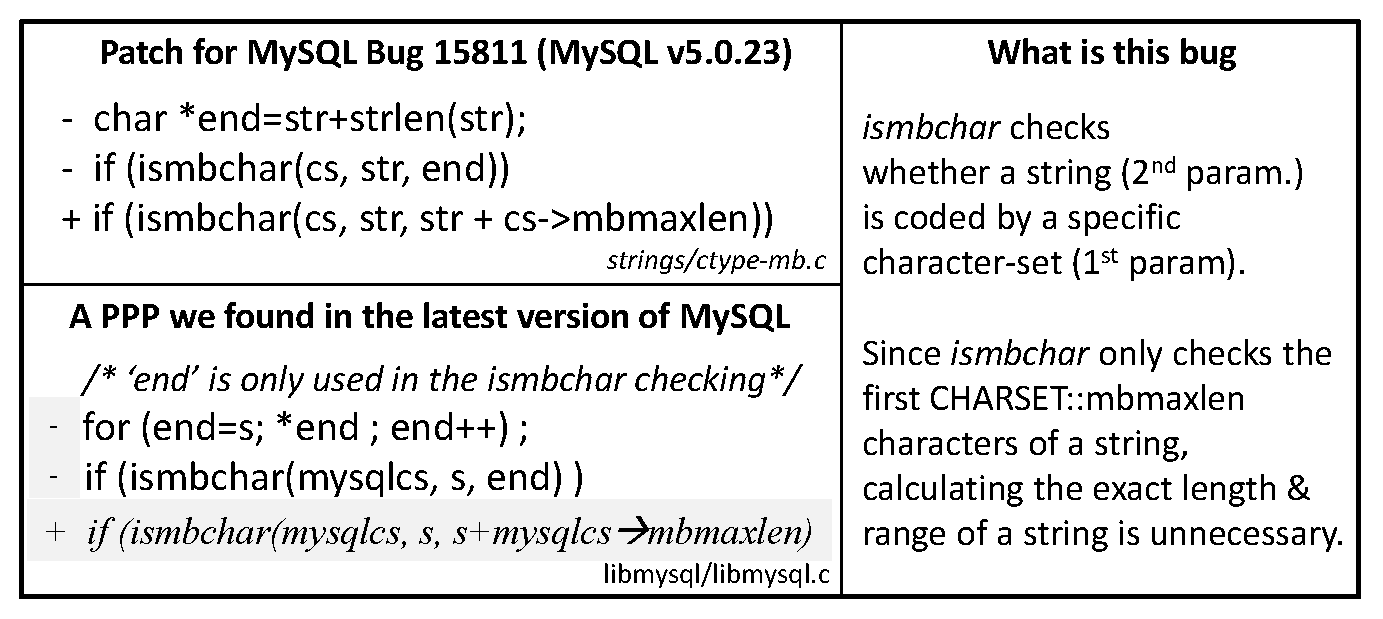
\includegraphics[height=1.42in]{figures/mysql15811.eps}
%\caption{\small PPP found in the same application}
%\label{fig:my15811}
\end{minipage}
\begin{minipage}{3in}
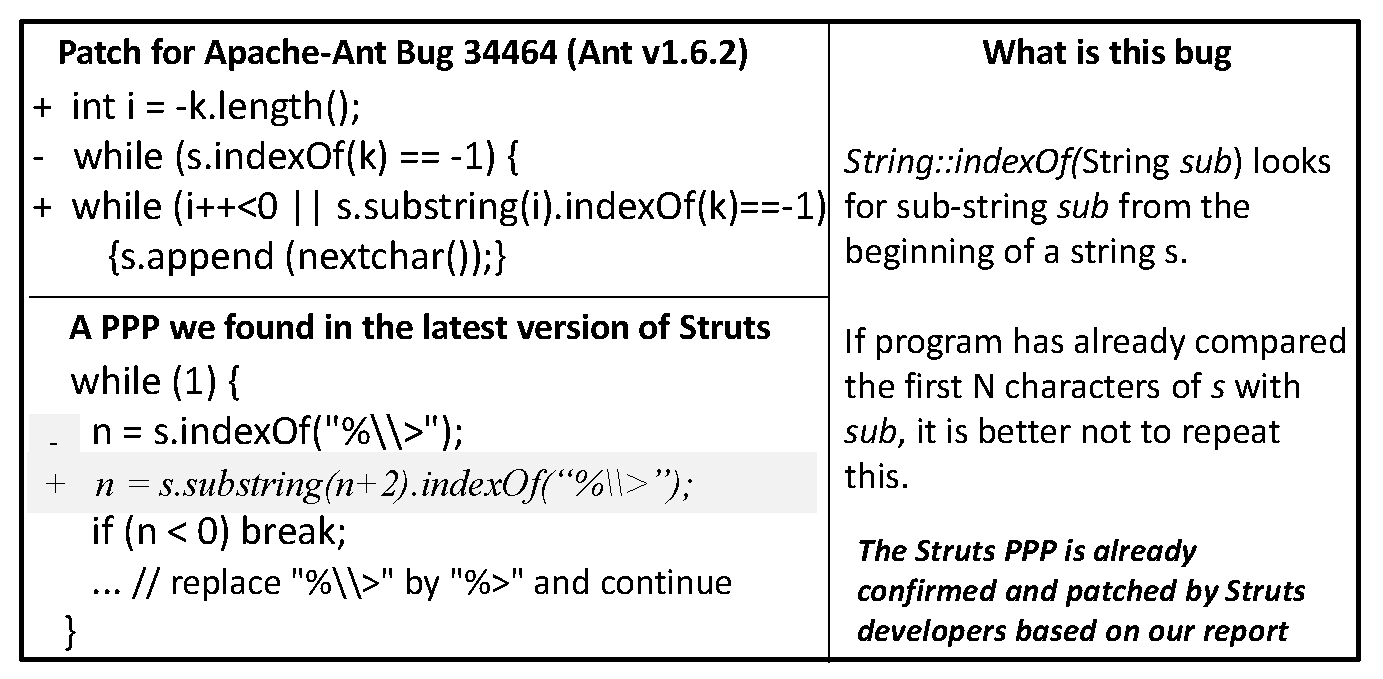
\includegraphics[height=1.42in]{figures/apache34464.eps}
%\caption{\small PPP found in a different application}
%\label{fig:ap34464}
\end{minipage}
\end{center}
\caption{PPPs we found in latest versions of {\it original} and {\it
different} software (the gray area shows how these two PPPs should be fixed)}
\label{fig:newbug}
\end{figure*}

{\bf PPPs In Original Versions\ }
17 out of 25 checkers found new PPPs, 125 in total, in the original versions
of the buggy software.
%that were missed by developers.

Some developers clearly tried to find all similar bugs when
fixing one bug, but did not succeed.
For example, in MySQL14637, after two buggy code regions were 
reported, developers found three more places that were similarly
inefficient and fixed them altogether. Unfortunately,
there were another 50 code regions that violated the same efficiency
rule and skipped developers' checking, as shown in 
Table~\ref{tab:result}. Similarly, MySQL developers found and fixed 3 places
that had the inefficiency pattern shown in Figure~\ref{fig:newbug},
but missed the other 15 places.

113 out of these 125 PPPs exist in different files or even different 
modules where the original bugs exist, which is probably why they were missed by
developers. These PPPs end up in several ways:
(1) 4 of them were fixed in later versions, which took 14--31 months;
(2) 20 eventually disappeared, because the
functions containing these PPPs were removed or re-implemented;
(3) 101 still exist in the latest versions of the software, wasting
computation resources 12--89 months after the original bugs were fixed.

\underline{Lesson\ } 
The above results show that developers do need support to systematically and 
automatically find similar performance bugs and fix them all at 
once.

{\bf PPPs In The Latest Versions\ }
2 of the 25 checkers are no longer applicable in the latest versions,
because the functions involved in these checkers
have been removed. The remaining 23 checkers are applied to
the latest versions of corresponding software and find
113 PPPs. Among them, 101 PPPs were
inherited from the original buggy versions.
The other 12 were introduced later. 

\underline{Lesson\ }
Developers cannot completely avoid the mistakes they made
and corrected before, which is understandable considering the large number of bugs in
software.
Specification systems and automated checkers can prevent developers 
from introducing old bugs into new code.
%programmers are still making the old mistakes. 

{\bf PPPs In Different Software Applications\ }
An exciting result is that 8 out of 13 cross-application checkers 
have successfully found previously unknown
PPPs in the latest versions of applications that are different from
where the rules came from.

Most of these checkers reflect common pitfalls in using
library functions. For example, Figure~\ref{fig:newbug} shows a pitfall
of using \Code{String::indexof()}. Apache-Ant developers made this
mistake, and we found Apache-Struts developers also made a similar mistake.

Apache32546 checker presents an interesting case. In the original 
bug report, developers from Apache-Slide recognized that
a small buffer size would severely hurt the performance of 
\Code{java.io.InputStream.read (byte buffer[])}
for reasonably large input
(e.g., larger than 50KB). Replacing their original
2KB buffer with a 200KB buffer achieved {\bf 80 times} throughput 
improvement in WebDav server. We first confirmed that this rule is
still valid. Our checker then found 135 places
in the latest versions of 36 software applications where similar mistakes were made.
These places use small buffers (1KB -- 4KB) to read images or data
files from disk or web, and are doomed to performance losses.

Some checkers reflect algorithm improvements and are also applicable to
many applications. For example, algorithm improvements for string operations 
proposed by MySQL developers (MySQL14637 and MySQL49491) also apply for
Mozilla and Apache HTTPD.


Cross-application checking also helps validate efficiency rules.
For example, by comparing how \Code{java.util.zip.Deflater.deflate()}
is used across applications, we found that Ant developers'
understanding of this API, reflected by their discussion, 
was wrong. They fixed Apache45396 by coincidence.

\underline{Lesson\ } 
The above results show that there exist general inefficiency patterns that
go beyond one application, just like that for functional
bugs \citep{billpugh}. 
Maintaining specifications and checkers for these general patterns can 
significantly save developers' effort, and allow them
to learn from other developers and other software. 
We can even discover performance bugs in a software where no
performance patch has ever been filed.
%TODO: software project, software application, confusing term.

\vspace{0.05in}
{\bf Bad Practices\ } 
Other than PPPs, some code regions identified by the 
checkers are categorized as bad practices.
For example, there are code regions very similar to
the MySQL PPP shown in Figure~\ref{fig:newbug}, except that the calculation of
\Code{end} is not completely useless as \Code{end} is used in places other than 
the invocation of \Code{ismbchar}.
Clearly this practice is more likely to cause performance problems
in the future than directly using
\Code{mysqlcs}$\rightarrow$\Code{mbmaxlen} as the parameter
for \Code{ismbchar} function.

\vspace{0.05in}
{\bf Good Practices\ }
Code regions that have well followed the efficiency rules are also identified
by slightly changed checkers.
For example, we found that in 13 places of various applications 
developers do use 
\Code{InputStream.read (byte buffer[])} in a performance efficient
way: \Code{buffer} has a configurable size or 
a large size that suits the workload (e.g., 64K in some Hadoop code).

\underline{Lesson\ } Violations to efficiency rules are not 
always rare comparing with good practices. 
Previous techniques that use statistical analysis to
infer functional rules \citep{PRMiner05,engler01bugs} 
may not work for efficiency rules.

{\bf False Positives\ }
Our PPP detection is accurate. 
On average, the false-positive-vs-PPP rate is 1:4.
The false positives mainly come from three sources.

First, Python checkers have no object-type information.
Therefore, some rules are applied to functions
with right function names but wrong classes
(e.g., Mozilla490742 and 
Apache32546). This is not a problem in LLVM checkers.

Second, some non-function rules are difficult to 
accurately express and check, which leads to false positives in
MySQL14637.

Third, accurately checking some efficiency rules requires run-time and/or 
workload information, which inevitably leads to false positives in
our static checkers. 
%This includes
%how many times a function is to be invoked, whether
%multiple threads could invoke a function concurrently, what is the typical
%length of an input, etc. 
False positives in Apache44408 and Apache48778 mostly belong to this 
category. These false positives can be largely eliminated by
run-time checkers.

{\bf Performance Results\ }
Our checkers are efficient. Each Python checker finishes
checking 10 million lines of code within 90 seconds.
Our LLVM checkers are mainly applied to 
MySQL, Mozilla Firefox, and Apache HTTPD.
It takes 4 -- 1270 seconds for one LLVM
checker to process one application.

We tried unit testing on PPPs.
The performance difference is significant. 
For example, for programs that read images and files using
\Code{InputStream.read}\Code{(byte buffer[])} with a 4KB-buffer parameter,
we can stably get 3 times throughput improvement through a 40K-buffer parameter.
When we feed the unit test with a 50MB file, which is a quite common image-file
workload these days,
the file operation time decreases from 0.87 second to 0.26 second,
a definitely perceivable difference.
As another example, the Struts code shown in Figure~\ref{fig:newbug}
is from a utility function used for processing JSP files. 
Our unit testing with a 15K JSP 
file shows that the simple patch can decrease latency by 0.1 second, 
a perceivable difference in interactive web applications.

Whole system testing turns out to be difficult, as suggested by our
characteristics study (Section~\ref{sec:char_exp}). 
No PPP detected by our checkers belongs to the always-active category. 
Future performance-oriented input-generation tools will significantly
help performance testing and identify truly severe PPPs. Execution frequency
information can also help future static performance-bug detectors to rank 
the severity of PPPs.

%TODO Our experience with developers. (1) If the patch is simple enough, 
%developers would do it.


\subsection{Discussions}

%TODO 1. original tone is too negative; should we put this earlier
%to lower the expectation?
{\bf Effectiveness of rule-based performance-bug detection\ }

{\it Effort saving\ } Rule-based detection not only identifies problems, but
also suggests alternative implementations with better efficiency.
These alternative implementations often
have small sizes and regular patterns,
as shown in Figure~\ref{fig:newbug}, 
making PPP validation and fixing easy.
It is also conceivable to enhance our checkers for automated PPP fixing. 

{\it Improving performance\ }
These PPPs showed 
significant performance improvement than their alternative implementations
in our unit testing. Without fixing these PPPs,
these unit-level performance losses could aggregate into intolerable
performance problems that are difficult to diagnose. 
This is especially significant considering that many performance bugs are
difficult to catch using other approaches.


{\it Maintaining code readability\ }
Like those 109 patches studied earlier, 
most PPPs detected by us can be fixed through changes to a few lines of code,
%and do not hurt code readability, 
as shown in Figure~\ref{fig:newbug}.
Even for the few complicated PPPs, wrapper-functions or 
macros can easily address the patch-readability issue.
%which is exactly what developers did in some of the patches we studied.

{\it Other usage\ }
Rules and checkers can serve as performance specifications for future 
software
development. They can aid in code maintenance when software evolves.
Developers can also save PPPs to an inefficiency list for future performance 
diagnosis.

Of course, this is only a starting point for rule-based performance-bug
detection. We expect our experience to motivate future work on 
automatically generating rules, checkers, or even patches.

%TODO you can automatically un-fix if you want
%TODO PPP xx is different from premature over-optimization.

\vspace{0.1in}
{\bf Can these problems be detected by other tools?\ }

{\it Copy-paste detectors\ } 
Most PPPs that we found are {\bf not} from copy-paste code regions
 and cannot be detected by text-matching tools
\citep{zhendong.oopsla10,CPMiner04}, as we can see in
Figure~\ref{fig:newbug}. Rule violations are not rare.
When developers misunderstand an API,
they tend to make mistakes whenever they use this API.
As a result, these mistakes usually go beyond
copy-paste code regions.

{\it Compiler optimization\ }
None of the bugs that provided the efficiency rules could be optimized
away by compilers used in Apache, MySQL, and Mozilla. Many PPPs 
involve library functions and algorithmic inefficiency, and
are almost impossible for a compiler to optimize
(Figure~\ref{fig:newbug}).
Even for the few cases where compiler optimization might help
(Figure~\ref{fig:emp}), 
the required inter-procedural and points-to analyses are not scalable
for real-world large software. 

{\it General rule-based bug detectors\ }
Ideas for detecting functional bugs can greatly benefit 
and inspire future research on performance bug detection.
However, many approaches cannot be directly applied.
Tools that automatically infer functional correctness rules 
\citep{engler01bugs,PRMiner05,livshits05dynamine} may not be suitable
for efficiency rules, because rule violations are not rare,
as shown in Table~\ref{tab:result}. In addition, many efficiency rules either
involve only one function or discourage multiple functions to be used together, 
making them unsuitable for tools that focus on function correlations. 


%TODO: gunami work infer complexity, ras bodik: 


%TODO: these are potential performance problems.
% how to use them: they might conflict with productivity, readability
% it could be better done by macro, wrapper, use for diagnosis



\chapter[Statistical Debugging for Real-World Performance Bugs]{Statistical Debugging for Real-World Performance Bugs}
\label{chap:sd}

TODO

\section{Introduction}

\subsection{Motivation}

%Performance bugs are implementation or design 
%defects in software can lead to inefficient 
%computation, causing unnecessary performance losses at run time.
%Previous studies have shown that performance bugs widely exist in the real-world~\citep{s2e,perf.fse10,rily.perftest,perfantipattern}.
%As we discussed in Chapter~\ref{chap:study}, 
%performance bugs are difficult for developers to avoid due to the lack of 
%performance documentation of APIs and the quickly changing workload of
%modern software, and a lot of performance bugs escape the in-house testing and manifest during production runs, 
%causing severe performance degradation and huge energy 
%waste in the field. 
%Making things worse, the negative impact of 
%these performance problems is getting increasingly important,
%with the increasing complexity of modern software and workload,
%the meager increases of single-core hardware performance, and the 
%pressing energy concerns.
%Effective techniques to diagnose real-world performance problems 
%are sorely needed.

As we discussed in Chapter~\ref{chap:study}, 
performance bugs are difficult to avoid during implementation, 
and are also difficult to expose during in-house testing. 
Many performance bugs manifest in front of end users 
and severely hurt users' experience during production runs. 
After users report performance bugs, 
developers need to quickly diagnose them and fix them. 
Diagnosing user-reported performance bugs is one important aspect to combat performance bugs. 
Effective tool support is sorely needed.

The state of practice of performance diagnosis is preliminary.
The most commonly used and often the only available tool during
diagnosis is profiler~\citep{oprofile,gprof}. 
Although useful, profilers are far from sufficient.
They can tell where
computation resources are spent, but not where or \textit{why} computation 
resources are 
\textit{wasted}.
As a result, they still demand a huge amount of manual effort to figure
out the root cause\footnote{Root cause refers to a static code
region that can cause inefficient execution.} of performance problems.

Figure~\ref{fig:MySQL26527}
shows a real-world performance problem in MySQL. MySQL users noticed 
surprisingly poor performance for queries on certain type of tables.
Profiling could not
provide any useful information, as the top ranked
functions are either low-level library functions, like 
\texttt{pthread\_getspecific} and \texttt{pthread\_mutex\_lock}, or simple 
utility
functions, like \texttt{ha\_key\_cmp} (key comparison). 
After thorough code inspection, developers finally figured
out that the problem is in function \texttt{start\_bulk\_insert}, which does
not even get ranked by the profiler.
The developer who implemented this
function assumed that parameter-0 indicates no need of cache, while the 
developers who 
wrote the caller functions thought that parameter-0 indicates the allocation of a
large buffer. This mis-communication led to unexpected cache-less execution, 
which is extremely slow. The final patch simply removes the unnecessary
branch in Figure~\ref{fig:MySQL26527}, but it took developers a lot of 
effort to figure out. 

Most recently, non-profiling tools have been proposed to help diagnose certain
type of performance problems. For example, X-Ray can help pin-point the 
configuration entry or input entry that is most responsible for poor 
performance~\citep{XRayOSDI}; trace analysis
techniques have been proposed to figure out the performance-causality 
relationship among system events and components~\citep{TaoAsplos2014,amertrace}. 
Although promising, these tools are still
far from automatically identifying
source-code level root causes and helping figure out
source-code level fix
strategies for general performance problems.

Many automated performance-bug detection tools have been proposed recently,
but they are ill suited for performance diagnosis.
Each of these tools detects one specific type of performance bugs,
such as inefficient nested loops~\citep{Alabama}, under-utilized data 
structures~\citep{XuDataStructure}, 
and temporary object bloat~\citep{BloatFSE2008, XuBloatPLDI2009, XuBloatPLDI2010},
through static or dynamic program analysis. They are not designed to cover a wide variety
of performance bugs. They are also not designed to focus on any specific
performance symptom reported by end users, and would inevitably lead to false 
positives when
used for failure diagnosis.


\subsection{Can we learn from functional failure diagnosis?}
\label{sec:5_canwe}
Automated failure diagnosis has been studied for decades for functional 
bugs
%\footnote{Any software defects that lead to functional misbehavior,
%such as incorrect outputs, crashes, and hangs. They include
%semantic bugs, memory bugs, concurrency bugs, and others.}. 
Many useful and generic techniques~\citep{horwitz, xiangyu.ase05, delta,liblit03,CCI,tarantula1} have been proposed.
Among these techniques,
statistical debugging is one of the most effective~\citep{liblit03,CCI,tarantula1}. 
Specifically, statistical debugging
collects program predicates, such as
whether a branch is taken, during both success runs and failure runs, and
then uses
statistical models to automatically identify predicates that are most
correlated with a failure, referred to as failure predictors.
It would be nice if statistical debugging can also work for diagnosing
performance problems.

Whether statistical debugging is useful for performance bugs is 
still an open question. Whether it is \textit{feasible} to apply
the statistical debugging technique to performance problems is unclear, 
not to mention 
\textit{how} to apply the technique.

\paragraph{Is it feasible to apply statistical debugging?}
The prerequisites for statistical debugging are two sets of inputs, one
leading to success runs, referred to as \emph{good inputs}, and one leading to 
failure runs, referred to as \emph{bad inputs}.
They are easy to obtain for functional bugs, but may be difficult for some
performance bugs.

For functional bugs, failure runs are often easy to tell from success runs 
due to clear-cut failure symptoms, such as 
crashes, assertion violations, incorrect outputs, and hangs. Consequently, 
it is straightforward to collect good and bad inputs. 
In the past, the main research challenge has been generating good inputs and 
bad inputs
that are similar with each other~\citep{delta}, which can improve the diagnosis
quality.

For some performance bugs, failure runs could be difficult to distinguish
from success runs, because execution slowness can be
caused by either large workload or manifestation of performance bugs.

Empirical study is needed to understand whether statistical debugging is feasible
for real-world performance bugs and, if feasible, how to obtain good inputs and
bad inputs.

\paragraph{How to conduct effective statistical debugging?}
The effectiveness of statistical debugging is not guaranteed by the
availability of good and bad inputs. Instead, it requires careful design
of predicates and statistical models that are suitable for the problem
under diagnosis.

Different predicates and
statistical models have been designed to target different types of common
functional bugs. 
For example, branch predicates and function-return predicates have been
designed to diagnose sequential bugs~\citep{liblit03,liblit05}; 
interleaving-related predicates have been designed to diagnose concurrency bugs~\citep{CCI,joy.asplos13}; 
$\Delta$LDA statistical model~\citep{Delta-LDA} has
been used to locate failure root causes that have weak signals.
What type of predicates and statistical models, if any, would work well
for performance diagnosis is still
an open question.

\subsection{Contributions}
This chapter presents a thorough study of statistical debugging for real-world 
performance 
problems. Specifically, it makes the following contributions.

\paragraph{An empirical study of the diagnosis process of real-world 
user-reported performance problems}  
To understand whether it is feasible to apply statistical debugging for
real-world performance problems, we study how users notice and report
performance problems based
on 65 real-world user-reported performance
problems in five representative open-source applications (Apache, Chrome, 
GCC, Mozilla, and MySQL).
We find that statistical debugging is feasible for most
user-reported performance problems in our study, because
(1) users notice the symptoms of most 
performance problems through a comparison-based approach 
(more than 80\% of the cases), and
(2) many users report performance bugs together with two sets of inputs that
look similar with each other but lead to %significantly different performance
huge performance difference
(about 60\% of the cases).
Furthermore, we also find that performance diagnosis is time consuming,
taking more than 100 days on average,
and lacking good tool support, taking more than 100 days on average even after 
profiling. 
Although our work is far from a full-blown study of all real-world
user-reported performance bugs, its
findings still provide guidance and motivation
for statistical debugging on performance problems. The details are 
in Section~\ref{sec:5_study}.

\paragraph{A thorough study of statistical in-house performance diagnosis}
To understand how to conduct effective statistical debugging for real-world
performance problems, we set up a statistical debugging framework and evaluate
a set of design points for user-reported performance problems. These
design points include
three representative predicates (branches, function returns, and scalar-pairs)
and two different types of statistical models. They are evaluated through 
experiments on 
20 user-reported performance problems and manual inspections on
all the 65 user-reported performance problems collected in our empirical study. 
Our evaluation
demonstrates that, when the right design points are chosen, statistical
debugging can effectively provide root-cause and fix-strategy information
for most real-world performance problems,
improving the state of the art of performance diagnosis. 
More details are presented
in Section~\ref{sec:5_inhouse}.

\paragraph{A thorough study of sampling-based production-run performance diagnosis}
We apply both hardware-based and software-based sampling techniques to
lower the overhead of statistical performance diagnosis.
Our evaluation using 20 real-world performance problems shows that
sampling does not degrade the diagnosis capability, while effectively
lowering the overhead to below 10\%. We also find that the special
nature of loop-related performance problems allows the sampling approach
to lower runtime overhead without extending the diagnosis latency,
a feat that is almost impossible to achieve for sampling-based
functional-bug failure diagnosis. More details are presented in Section~\ref{sec:5_lbr}.

\section{Understanding Real-World Performance Problem Reporting and Diagnosis}
\label{sec:5_study}

This section aims to understand the performance diagnosis process
in real world. Specifically, we will focus on these two aspects of
performance diagnosis.

\begin{enumerate}
\item How users notice and report performance problems.
This will help us understand the feasibility of applying statistical debugging
to real-world performance problems, as discussed in 
Section~\ref{sec:5_canwe}. Particularly, we will study how users
tell success runs from failure
runs in the context of performance bugs and how to obtain
success-run inputs (i.e., good inputs) and failure-run inputs
(i.e., bad inputs) for performance diagnosis.
\item How developers diagnose performance problems.
This will help us understand the state of practice of performance diagnosis.
\end{enumerate}

\subsection{Methodology}



\begin{table}[h!]
\centering
\scriptsize
\begin{tabular}{@{\hspace{3pt}}l@{\hspace{3pt}}@{\hspace{3pt}}c@{\hspace{3pt}}}
\toprule
Application Suite Description (language) & \# Bugs \\
\midrule
\bigstrut[t]                           
{\bf Apache Suite} 	 & 16\\
%\cline{1-1}
{HTTPD:	Web Server (C)	}& \\
{TomCat:  Web Application Server (Java)}& \\
{Ant:	Build management utility (Java)}& \\
%\hline
%JMeter	& Load test utility (Java) & \\
\midrule                            
{\bf Chromium Suite} Google Chrome browser (C/C++) & 5\\
\midrule
%\multicolumn{2}{|l|}
{\bf GCC Suite}  GCC \& G++ Compiler (C/C++)     & 9\\
\midrule
{\bf Mozilla Suite}  & 19\\
%\cline{1-1}
{Firefox: Web Browser (C++, JavaScript)}& 	\\
{Thunderbird: Email Client (C++, JavaScript)}& \\
\midrule
{\bf MySQL Suite}     & 16	\\
%\cline{1-1}
{Server: Database Server (C/C++)}&  	\\
%\cline{1}
{Connector: DB Client Libraries (C/C++/Java/.Net)} &  	\\
\midrule
{\bf Total}	   & 65 \\
\bottomrule
\end{tabular}
\caption{Applications and bugs used in the study}
\label{tab:app_bug}
\end{table}

\begin{table*}[tb!]
\begin{adjustwidth}{-1.5in}{-1.5in}
\scriptsize
\centering
{
\begin{tabular}{lcccccc}
\toprule
\multicolumn{1}{c}{Categories} &Apache&Chrome&GCC&Mozilla&MySQL&Total\\
\midrule
\multicolumn{1}{l}{\textbf{Comparison within one code base}}
&9&3&7&7&12&38\\
\ \ Comparing the same input with different configurations &2&1&1&1&5&10\\
\ \ Comparing inputs with different sizes&6&2&4&4&6&22\\
\ \ Comparing inputs with slightly different functionality&2&0&3&2&4&11\\
\midrule
\multicolumn{1}{l}{\textbf{Comparison cross multiple code bases}}
&7&3&8&5&4&27\\
\ \ Comparing the same input under same application's different versions
&4&2&8&3&3&20\\
\ \ Comparing the same input under different applications
&4&1&1&2&1&9\\
\midrule
\multicolumn{1}{l}{\textbf{Not using comparison-based methods}}
&3&1&0&9&1&14\\
\bottomrule
\end{tabular}
}
\end{adjustwidth}
\caption{How performance problems are observed by end users (There are overlaps among
    different comparison-based categories; there is no overlap between non-comparison
    and comparison-based categories)}
\label{tab:cmp}
\end{table*}

The performance problems under this study include all user-reported
performance problems from a real-world performance-bug benchmark suite 
collected by 
previous work~\citep{PerfBug}. We briefly discuss this baseline benchmark
suite and our refinement below.

The baseline benchmarks~\citep{PerfBug} contain 110 fixed real-world performance
bugs randomly sampled from five representative open-source software suites.
These five software suites are all large and mature,
with millions lines of codes and well maintained bug databases. 
They also provide a good coverage of different types of software projects, as
shown in Table~\ref{tab:app_bug}.
The 110 bugs contained in this baseline suite are from
on-line bug databases and are tagged by developers as performance
bugs.

We cannot directly use this baseline benchmark suite, because it contains
bugs that are discovered by developers themselves through code inspection, a
scenario that performance diagnosis does not apply.
Consequently, we carefully read through all the bug reports and identify all 
the \textbf{65} bugs that are clearly reported by users.
These 65 bug reports all contain detailed information about how each 
performance problem is observed by a user and gets diagnosed by developers.
They are the target of the following characteristics study, and will be 
referred to as \textit{user-reported performance problems} or 
simply \textit{performance problems} in the remainder of this paper.
The detailed distribution of these 65 bugs is shown in Table~\ref{tab:app_bug}.




\paragraph{Caveats} 
Similar with all previous characteristics studies, our findings and 
conclusions need to be considered with our methodology in mind. 
The applications in our study cover a variety of important software categories, 
workload, development background, and programming languages. However, there are
still uncovered categories, such as scientific computing software and 
distributed systems.

The bugs in our study are collected from an earlier benchmark suite 
\citep{PerfBug} without bias. 
We have followed users and developers' discussion to decide what are 
performance problems that are noticed and reported by users, and finally
diagnosed and fixed by developers.
We did not intentionally ignore any aspect of performance problems. 
Of course, our study does not cover performance problems that are 
not reported to or fixed in the bug databases. It also does not cover
performance problems that are indeed reported by users but have undocumented
discovery and diagnosis histories.
Unfortunately, there is no conceivable way to solve these problems.
We believe the bugs in our study provide a representative sample of the 
well-documented fixed
performance bugs that are reported by users in representative applications.


\begin{table*}[tb!]
\begin{adjustwidth}{-1.5in}{-1.5in}
\scriptsize
\centering
{
\begin{tabular}{lcccccc}
\toprule
\multicolumn{1}{c}{Categories} &Apache&Chrome&GCC&Mozilla&MySQL&Total\\
\midrule
\multicolumn{1}{l}{\textbf{Comparison within one code base}}
&9&3&7&7&12&38\\
\ \ Comparing the same input with different configurations &2&1&1&1&5&10\\
\ \ Comparing inputs with different sizes&6&2&4&4&6&22\\
\ \ Comparing inputs with slightly different functionality&2&0&3&2&4&11\\
\midrule
\multicolumn{1}{l}{\textbf{Comparison cross multiple code bases}}
&7&3&8&5&4&27\\
\ \ Comparing the same input under same application's different versions
&4&2&8&3&3&20\\
\ \ Comparing the same input under different applications
&4&1&1&2&1&9\\
\midrule
\multicolumn{1}{l}{\textbf{Not using comparison-based methods}}
&3&1&0&9&1&14\\
\bottomrule
\end{tabular}
}
\end{adjustwidth}
\caption{How performance problems are observed by end users (There are overlaps among
    different comparison-based categories; there is no overlap between non-comparison
    and comparison-based categories.).}
\label{tab:5_cmp}
\end{table*}







\subsection{How users report performance problems}
In general, to conduct software failure diagnosis, it is critical to understand 
what are the failure symptoms and what information is available for failure
diagnosis. 
Specifically, as discussed in Section~\ref{sec:5_canwe}, to understand the
feasibility of applying statistical debugging for performance diagnosis, we
will investigate two issues: (1)
How do users judge whether a slow execution is caused by large workload or
inefficient implementation, telling success runs from failure
runs?
(2)
What information do users provide to convince developers that inefficient
implementation exists and hence help the performance diagnosis?

\paragraph{How are performance problems observed?}

As shown in Table~\ref{tab:5_cmp}, the majority (51 out of 65) of user-reported 
performance problems are observed through comparison, including
comparisons within one software code base and comparisons across multiple code bases.

\underline{\it Comparison within one code base} 
is the most common way to reveal performance problems.  
In about 60\% of cases, 
users notice huge performance differences among
similar inputs and hence file bug reports.

Sometimes, the inputs under comparison have the same functionality but different
sizes. For example, MySQL\#44723 is reported when users observe that inserting
11 rows of data for 9 times is two times slower than inserting 9 rows of data
for 11 times. As another example, Mozilla\#104328 is reported when users observe
a super-linear performance degradation of the web-browser start-up time in terms
of the number of bookmarks.

Sometimes, the inputs under comparison are doing slightly different tasks.
For example, when reporting Mozilla\#499447, the user mentions that changing the width
of Firefox window, with a specific webpage open, takes a lot of time (a bad input), yet
changing the height of Firefox window, with the same webpage,
takes little time (a good 
input).

%Finally, significantly different performances under the same input and different 
Finally, large performance difference under the same input and different
configurations is also a common reason for users to file bug reports.
For example, when reporting GCC\#34400, the user compared the compilation time
of the same file under two slightly different GCC configurations.
The only difference between these two configurations is that the ``ZCX\_By\_Default''
entry in the configuration file is switched from True to False. 
However, the compilation times goes from 4 seconds to almost 300 minutes.

\underline{\it Comparison across different code bases} 
In about 40\% of the performance problems that we studied, users support
their performance suspicion through a comparison 
across different code bases. For example, GCC\#12322 bug report mentions
that ``GCC-3.3 compiles this file in about five minutes; GCC-3.4 takes
30 or more minutes''. As another example, Mozilla\#515287 bug report
mentions that the same Gmail instance leads to 15--20\% CPU utilization
in Mozilla Firefox and only 1.5\% CPU utilization in Safari.

Note that, the above two comparison approaches do not exclude each other.
In 14 out of 27 cases, comparison results across multiple code bases are reported
together with comparison results within one code base.

\underline{\it Non-comparison based}
For about 20\% of user-reported performance problems, users observe an
absolutely non-tolerable performance and file the bug report without any comparison.
For example, Mozilla\#299742 is reported as the web-browser frozed to crawl.

\paragraph{What information is provided for diagnosis?}

\begin{table*}[tb!]
\begin{adjustwidth}{-.5in}{-.5in}
\scriptsize
\centering
{
\begin{tabular}{lcccccc}
\toprule
&Apache&Chrome&GCC&Mozilla&MySQL&Total\\
\midrule
Total \# of bug reports & 16 & 5 & 9 & 19 & 16 & 65 \\
\midrule
\multicolumn{7}{c}{\bf \# of bad inputs provided}\\
\multicolumn{1}{l}{{\bf 0/?}: No bad input }
&0&0&0&0&0&0\\
\multicolumn{1}{l}{{\bf 1/?}: One bad input}
&0&1&5&6&7&19\\
\multicolumn{1}{l}{{\bf n/?}: A set of bad inputs}
&16&4&4&13&9&46\\
\midrule
\multicolumn{7}{c}{\bf \# of good inputs}\\
\multicolumn{1}{l}{{\bf ?/0}: No good input}
&7&2&2&12&4&27\\
\multicolumn{1}{l}{{\bf ?/1}: One good input}
&0&0&3&0&3&6\\
\multicolumn{1}{l}{{\bf ?/n}: A set of good inputs}
&9&3&4&7&9&32\\
\bottomrule
\end{tabular}
}
\end{adjustwidth}
\caption{Inputs provided in users' bug reports ($n$: 
developers provide a way to generate a large number of inputs.).}
\label{tab:5_input}
\end{table*}

The most useful information provided by users include failure
symptom (discussed above), bad inputs, and good inputs. Here, we refer to the 
inputs that lead to user-observed performance problems
as \textit{bad inputs}; we refer to the
inputs that look similar with some bad inputs but lead to good performance,
according to the users,
as \textit{good inputs}.

\underline{\it Bad inputs} Not surprisingly, users provide problem-triggering
inputs in all the 65 cases. What is interesting is that in about 70\% of
cases (46 out of 65), users describe a category of inputs, instead of just
one input, that can trigger
the performance problem, as shown in Table \ref{tab:5_input}. For example,
in MySQL\#26527, the user describes that loading data from file into partitioned
table can trigger the performance problem, no matter what is the content or 
schema of the table. 

\underline{\it Good inputs} Interestingly, good inputs are specified in almost
60\% of bug reports, as shown in Table \ref{tab:5_input}. 
That is, users describe inputs that look similar with the
bad inputs but have much better performance in all the 38 bug reports
where ``comparison within one code base'' is used to observe the performance
problem.
Furthermore,
in 32 bug reports, users describe how to generate a large number of good
inputs, instead of just one good input.
For example, when reporting MySQL\#42649, the user
describes that executing queries on tables using the default charset setting or
the \textit{latin1} charset setting (good inputs) will not cause lock contention, while queries
on tables using other types of charset settings (bad inputs) may cause lock contention.
Note that, this is much rarer in functional bug reports, which is why special
tools are
designed to automatically generate inputs that execute correctly
and are similar with bad inputs, when diagnosing functional-bug failures~\citep{delta}.

%\paragraph{Hypothesis Testing}

%We conduct several hypothesis testings to evaluate whether we have enough evidence to draw conclusions about performance bugs based on our sample. We choose 0.01 as significance level. 
%Under this setting, if we draw a conclusion, the conclusion only has 1\% probability to be wrong. 
%Our testing results show that more performance bugs are reported with a set of bad inputs, 
%but we fail to draw a conclusion that more performance bugs are reported with comparison-based methods. 


\subsection{How developers diagnose performance problems}

To collect the diagnosis time, we check the bug databases and calculate the
time between a bug report being posted and a correct fix being proposed.
Of course, strictly speaking, this time period can be further broken down to
bug-report assignment, root-cause locating, patch design, and so on. 
Unfortunately, we cannot obtain such fine-grained information accurately
from the databases. Most Apache, Chrome, and MySQL bugs in
our study do not have clear assignment time in record. For GCC bugs in
study, report assignment takes about 1\% of the overall diagnosis
time on average; for Mozilla bugs in study, report assignment takes about
19\% of the overall diagnosis time on average.

Our study shows that it takes 129 days on average for developers to finish
diagnosing a performance problem reported by users.
Among the 5 software projects, the Chrome project has the shortest average
performance-diagnosis time (59 days), and Apache project has the longest
average diagnosis time (194 days).
Comparing with the numbers reported in Chapter~\ref{chap:study}, 
the time to diagnose user-reported performance problems is slightly shorter
than that for non-user-reported performance problems,
and similar or longer than that of 
functional bugs. 

We also studied how developers diagnose performance problems.
The only type of diagnosis tools that are mentioned in bug reports are
performance profilers. They are mentioned in 13 out of the 65 reports.
However, even after the profiling results are provided, it still takes
developers 116 days on average to figure out the patches.


\subsection{Implications of the study}
\label{sec:5_study_imp}

\ \ \underline{\textit{Implication 1}}
Performance bugs and functional bugs are observed in different ways.
Intuitively, the symptoms of many functional bugs, such as assertion violations,
error messages, and crashes, can be easily identified by looking
at the failure run alone~\citep{LiASID06}.
In contrast, the manifestation
of performance bugs often gets noticed through comparison.
%TODO check functional bugs and conduct a statistical test here
We have randomly sampled 65 user-reported functional bugs from the same set
of applications (i.e., Apache, Chrome, GCC, Mozilla, and MySQL) and found that
only 8 of them are observed through comparison.
Statistical Z tests~\citep{ztest} show that the above observation is 
statistically
significant --- at the 99\% confidence level, 
a user-reported performance bug is more likely to be observed through 
comparison than a user-reported functional bug.

\underline{\textit{Implication 2}}
Although judging execution efficiency based on execution time alone 
is difficult in
general, distinguishing failure runs from success runs and obtaining bad and good
inputs are fairly straightforward based on performance-bug reports filed by 
users.
Our study shows that most user-reported performance problems are observed when 
two sets of similar inputs demonstrate very different performances (38 out of 
65 cases). 
Most of these cases (32 out of 38), users provide explicit good and bad 
input-generation methodology. 
In other cases (27 out of 65),
users observe that an input causes intolerably slow execution or very different
performances across similar code bases. Distinguishing
failure runs from success runs and bad inputs from good inputs are 
straightforward in these cases based on the symptoms described
in the bug reports, such as ``frozed the GUI to
crawl'' in Mozilla\#299742 and 10X more CPU utilization rate than Safari 
under the same input in Mozilla\#515287. 

\underline{\textit{Implication 3}}
Statistical debugging is naturally suitable for diagnosing many
user-reported performance problems,
because most performance bugs are observed by users through comparison and many
performance-bug reports (38 out of 65) already contain information about 
both bad and good inputs that are similar with each other.
Statistical tests~\citep{ztest} show that with 90\% statistical confidence, 
a user-filed performance-bug report is more likely to contain both 
bad and good inputs than not.
Comparing the 65 randomly sampled functional bugs mentioned above with the 65
performance bugs, 
statistical tests~\citep{ztest} show that, at the 99\% confidence level, 
a user-filed performance-bug report is more likely to contain
good inputs than a user-filed
functional-bug report.
Previous statistical debugging work tries hard to generate good
inputs to diagnose functional bugs~\citep{delta}. This task is
likely easier for performance failure diagnosis.

\underline{\textit{Implication 4}}
Developers need tools, in addition to profilers, to diagnose
user-reported performance problems.

\section{In-house statistical debugging}
\label{sec:inhouse}
During in-house performance diagnosis, users send detailed bug reports to
the developers and developers often repeat the performance problems
observed by the users before they start debugging.
Following the study in Section~\ref{sec:study}, this section designs and
evaluates statistical debugging for in-house diagnosis of real-world
performance problems.
We aim to answer three key questions.

\begin{enumerate}
\item What statistical debugging design is most suitable for diagnosing
real-world performance problems;
\item What type of performance problems can be diagnosed by statistical
debugging;
\item What type of performance problems cannot be diagnosed by statistical
debugging alone.
\end{enumerate}

\subsection{Design}
In general, statistical debugging 
\citep{liblit03,liblit05,CCI,tarantula1,tarantula2,tarantula.darko,joy.asplos13}
is an approach that uses statistical machine learning techniques to help
failure diagnosis. It usually works in two steps.
First, a set of run-time 
events $E$ are collected from both success runs and failure runs.
Second, a statistical model is applied to identify an event $e \in E $
that is most correlated with the failure, referred to as the failure predictor. 
Effective statistical debugging can identify failure predictors that are
highly related to failure root causes and help developers fix the underlying
software defects.

There are three key questions in the design of statistical debugging.
\begin{enumerate}
\item Input design --
what inputs shall we use to drive the 
incorrect execution and the correct execution during statistical debugging.
If the good runs and the bad runs are completely different
(e.g., they do not cover any common code regions), the diagnosis will
be difficult.
\item Predicate design -- what type of run-time events shall we monitor.
Roughly speaking, a predicate $P_i$ could be true or false, depending on 
whether a specific property is satisfied at instruction $i$ at run time.
To support effective diagnosis, one should choose predicates that can reflect 
common failure root causes.
\item Statistical model design -- what statistical model shall we use to
rank predicates and identify the best failure predictors among them.
\end{enumerate}

The input design problem is naturally solved for performance diagnosis, as
discussed in Section \ref{sec:study}. We discuss different predicate designs
and statistical model designs below.

\subsubsection{Predicate designs}
Many predicates have been designed to diagnose functional bugs.
We discuss some commonly used ones below.

\paragraph{Branches.} There are two branch 
predicates associated
with each branch $b$: one is true when $b$ is taken, and the other is true when
$b$ is not taken~\citep{liblit03,liblit05}.

\paragraph{Returns.} There are a set of six return predicates
for each function return point, tracking whether the return value is ever
$<0$, $\leq 0$, $>0$, $\geq 0$, $=0$, or $\neq 0$ \citep{liblit03,liblit05}.
%negative, zero, or positive \cite{liblit03,liblit05}.

\paragraph{Scalar-pairs.} There are six scalar-pair predicates
for each pair of variables $x$ and $y$, tracking whether $x$ is ever 
$<y$, $\leq y$, $>y$, $\geq y$, $=y$, or $\neq y$ \citep{liblit03,liblit05}.
%smaller than,
%larger than, or equal to $y$ \cite{liblit03,liblit05}. 
Whenever a scalar
variable $x$ is updated, scalar-pair predicates are evaluated between $x$ and
each other same-type variable $y$ that is in scope, as well as program 
constants.

\paragraph{Instructions.} Instruction predicate $i$ is true, if 
$i$ has been executed during the monitored run 
\citep{tarantula1,tarantula2,tarantula.darko}.

\paragraph{Interleaving-related ones.} Previous work on diagnosing
concurrency bugs \citep{CCI} has designed three types of predicates that are 
related to
thread interleaving. For example, CCI-Prev predicates track whether two 
consecutive accesses to a
shared variable come from two distinct threads or the same thread.

In the remainder of this section, we will focus on three predicates: branch
predicates, return predicates, and scalar-pair predicates. We skip
instruction predicates in this study, because they are highly related to
branch predicates. We skip interleaving-related predicates in this study,
because most performance problems that we study are deterministic and
cannot be effectively diagnosed by interleaving-related 
predicates.

\begin{table*}
  \centering
  \scriptsize
  \newcommand{\Yes}[1]{\checkmark{}$_#1$}
  \newcommand{\No}[0]{-}
  \begin{adjustwidth}{-.15in}{-.15in}
  {
  \begin{tabular}{lccccccc}
    \toprule
              &          &         & \multicolumn{3}{c}{\bf Static \# of predicates}& {\bf Static \# of} & {\bf Reported Inputs}\\
    \cmidrule(lr){4-6}
     {\bf BugID}     &{\bf KLOC}   &{\bf Language}    &{\bf Branch}    &{\bf Return}   &{\bf Scalar-pair}   &{\bf Loops}    &{\bf (bad/good)} \\
    \midrule
    Mozilla258793    & 3482        & C++              & 385722         & 1126770       & *                & 10016         & n/0            \\
    Mozilla299742    & 3482        & C++              & 385720         & 1126698       & *                & 10016         & 1/0            \\
    Mozilla347306    & 88          & C                & 26804          & 38634         & 271968             & 951           & n/n            \\
    Mozilla416628    & 105         & C                & 28788          & 39306         & 302496             & 1420          & 1/0            \\
    \midrule
    MySQL15811       & 1149        & C++              & 13508          & 15576         & *                & 760           & n/n            \\
    MySQL26527       & 986         & C++              & 90128          & 128610        & *                & 4222          & n/n            \\
    MySQL27287       & 995         & C++              & 92316          & 119322        & *                & 4683          & n/n            \\
    MySQL40337       & 1191        & C++              & 103686         & 138582        & *                & 4510          & n/n            \\
    MySQL42649       & 1164        & C++              & 126822         & 155766        & *                & 5688          & n/n            \\
    MySQL44723       & 1164        & C++              & 126822         & 155766        & *                & 5688          & 1/1            \\
    \midrule
    Apache3278       & N/A         & Java             & 10             & 126           & 204                & 7             & n/n           \\
    Apache34464      & N/A         & Java             & 22             & 42            & 342                & 8             & n/n           \\
    Apache47223      & N/A         & Java             & 24             & 36            & 390                & 9             & n/n           \\
    Apache32546      & N/A         & Java             & 6              & 66            & 120                & 5             & n/n           \\
    \midrule
    GCC1687          & 2099        & C                &  183496 & 296058 & 4187586 & 6476     & n/n            \\
    GCC8805          & 2538        & C                &  207188 & 327804 & 4161012 & 7309     & n/n            \\
    GCC15209         & 2586        & C                &  192108 & 304800 & 3705558 & 7310     & 1/1            \\
    GCC21430         & 3844        & C                &  238514 & 447510 & 3768078 & 9078     & n/n            \\
    GCC46401         & 5521        & C                &  337810 & 713532 & 5625606 & 15159    & 1/1            \\
    GCC12322         & 2341        & C                &  177098 & 284484 & 3750912 & 6563     & 1/0            \\
    \bottomrule
   \end{tabular}
   }
   \end{adjustwidth}
  %\nocaptionrule
  \caption{Benchmark information. (N/A: since our statistical debugging tools 
      only work for C/C++ programs, we have 
	reimplemented the four Java benchmarks in C programs. *: we have no
	tools to collect scalar-pair predicates in C++ programs. 
	The 1s and $n$s in the
	``Reported Inputs'' column indicate how many bad/good inputs are reported
	by users.)}
  \label{tab:benchmarks}
\end{table*}

\subsubsection{Statistical model designs}
Many statistical models have been used before for anomaly 
detection \citep{engler01bugs,CPMiner04,kremenek06inferring,lamsigsoft02} 
and fault localization 
\citep{liblit03,liblit05,CCI,tarantula1,tarantula2,tarantula.darko,Delta-LDA}.
Although the exact models used by previous work differ from each other, they 
mostly follow the same principle --- if a predicate is a good failure predictor,
it should be true in many failure runs, and be false or not-observed
in many success runs. They can be roughly categorized into two classes.
The first class
only considers whether a predicate has been observed
true for at least once in a run (e.g., whether a branch $b$ has been
taken for at least once). The exact number of times the predicate has
been true in each run is not considered in the model.
The second class instead considers the exact number of times a predicate has 
been true in each run.
Naturally, by considering more information in the model, the second class could
complement the first class, but at the cost of longer processing time.
Most previous work on functional bug
diagnosis has found the first class sufficient 
\citep{liblit03,liblit05,CCI,joy.asplos13} and did not try 
the second class.

To cover both classes of statistical models for performance diagnosis, our 
study will look at two models: a
\emph{basic} model proposed by CBI work \citep{liblit03,liblit05} that belongs
to the first class discussed above 
and a $\Delta$LDA model proposed by \citep{Delta-LDA} that belongs
to the second class discussed above. 
We leave investigating other existing statistical
models and designing new models to future work. Since our evaluation will use
exactly the same formulas, parameters, and settings
for these two models as previous work \citep{liblit03,liblit05,Delta-LDA}, we
briefly discuss these two models below.
More details about these two models can be found in their
original papers \citep{liblit03,liblit05, Delta-LDA}. 

\paragraph{Basic model}
This model works in two steps.
First, it checks whether an execution is more likely to fail 
when a predicate $P$ is observed true, 
whose probability is computed by formula \textit{Failure}$(P)$, 
than when $P$ has merely being observed during the execution, 
whose probability is computed by formula \textit{Context}$(P)$.
Consequently, only predicates, whose \textit{Increase} values computed below
are higher than 0 with
certain statistical confidence, will appear in the final ranking list.
By default, statistical Z-tests and 0.99 confidence level are 
used in CBI \citep{liblit03}.

\[
Failure(P) =  \frac{F(P_{\text{true}})}{S(P_{\text{true}})+F(P_{\text{true}})}
\]

\[
Context(P) =  \frac{F(P_{\text{observed}})}{S(P_{\text{observed}})+F(P_{\text{observed}})}
\]

\[
Increase(P) =  Failure(P) - Context(P)
\]

$F(P_{\text{true}})$ is the number of failure runs in which P is true, 
and $F(P_{\text{observed}})$
is the number of failure runs in which P is observed, no matter true or false. 
$S(P_{\text{true}})$ is the number of success runs 
in which P is true, and $S(P_{\text{observed}})$
is the number of success runs in which P is observed. 

 
\[
Importance(P) =  \frac{2}{\frac{1}{Increase(P)} + \frac{1}{log(F(P_{\text{true}}))/log(F)}}
\]

The final ranking is based on an \textit{Importance} metric. This metric
reflects the harmonic mean of
the \textit{Increase} metric and the conditional probability of a predicate $P$
being true given that an execution has failed. 
$F$ is the total number of failure runs in the formula above.
Previous work 
\citep{liblit05}
has tried different
variants of the harmonic mean and found the formula above, with a logarithmic
transformation, to be the best. As mentioned above, we reuse all the formulas, 
parameters, and settings from previous work. 

\paragraph{$\Delta$LDA model}
$\Delta$LDA~\citep{Delta-LDA} model is derived from a famous machine learning
model, called Latent Dirichlet Allocation 
(LDA) \citep{LDA}.
By considering how many times a predicate is true 
in each run, it can pick up weaker bug signals, as shown by previous work \citep{Delta-LDA}.
Imagine the following scenario ---
during a success run, predicate $P$ is true for
10 times and false for 100 times; during a failure run, $P$ is true for 
100 times and false for 10 times. The basic model will consider $P$ as useless,
as it has been observed both true and false in every run. However, $\Delta$LDA model will 
notice that $P$ is true for many more times during each failure run than that in 
each success
run, and hence consider $P$ as failure predictor. The exact ranking formula of
$\Delta$LDA model is very complicated, and is skipped here. It can be found
in previous work \citep{Delta-LDA}.
  
\paragraph{How to apply the models}
A statistical debugging framework collects the following
information from each run: (1) whether the run has succeeded and failed;
%(2) a list of predicates that have been observed and for how many times each
%(the latter only for $\Delta$LDA model); 
(2) a list of predicates that have been observed true and for how many 
times each (the latter only for $\Delta$LDA model). 
After collecting such information from
several success runs and failure runs, the framework will naturally obtain
values, such as the number of failure runs where a predicate is observed/true,
for the formulas discussed above and produce a rank list of failure predictors.




\subsection{Experimental evaluation}
\label{sec:inhouse_results}
\subsubsection{Methodology}
\label{sec:inhouse_meth}
To evaluate how statistical debugging works for real-world performance problems,
we apply three types of predicates and two types of statistical models on 
real-world user-reported performance problems.
All our experiments are conducted on an Intel i7-4500U machine, with Linux 3.11 kernel.

\paragraph{Benchmark selection}
Among the 65 user-reported performance problems discussed in Section 
\ref{sec:study}, we have tried our best effort and successfully repeated 20
of them from four different C/C++/Java 
applications. In fact, most of the 65 performance problems are deterministically repeatable based on the bug reports.
We have failed to repeat 45 of them for this
study mainly because they depend on special hardware platforms or very
old libraries that are not available to us or very difficult to set up. 
The detailed information for the 20 performance problems used in our experiments 
is shown in Table~\ref{tab:benchmarks}.
Specifically, the static number of branch predicates is counted based on the 
fact that
there are two predicates for each static branch instruction in the user program
(excluding library code). The static numbers of other predicates are similarly
counted.
%For C (and Java) benchmarks, CBI will count these three numbers and put them in the final results automatically. 
%For C++ benchmarks, the number of branch predicates is the product of 2 
%and the number of conditional branch instruction inside each binary code, 
%and the number of return predicates is the product of 6 
%and the number of call sites whose return types are characters, 
%integers or pointers inside each binary code. 
%These are following the same instrumentation scheme inside CBI. 
%The 7th column shows the number of static loops inside each compiled binary code. 
%We get numbers in this column by implementing a simple counting tool based on Dyninst~\cite{dyninst}. 

To make sure these 20 benchmarks are representative, we also conduct
manual source-code inspection to see how statistical debugging could work
for \textbf{all} the 65 user-reported performance problems in our study. 
We will show that our
manual inspection results on all the 65 cases are \textbf{consistent} with
our experimental evaluation on these 20 benchmarks. 

%{\bf [Linhai also checked profiling ranks for functions containing the final patches. 
%For 7 bugs, functions containing final patches are not shown in the profiling ranking
%lists. For the rest of 13 bugs, the median of ranks for functions containing final patches is 19. ]}
%




\paragraph{Input design}
To conduct the statistical debugging, we run each benchmark program 20 times, using
10 unique good inputs and 10 unique bad inputs.
For each performance problem, we get its corresponding 20 inputs based on users'
bug report. For 13 of them, the bug reports have described
how to generate a large number of good and bad inputs, which makes our input
generation straightforward. For the remaining 7 bugs, with 3 from Mozilla, 3 
from GCC, and 1 from MySQL, we randomly
change the provided inputs and use the user-provided failure-symptom
information to decide which inputs are good or bad.
We make sure that inputs generated by us are still valid HTML webpages, valid JavaScript programs,
valid C programs, or valid database tables/queries.
The process of judging which inputs
are good or bad is straightforward,
as discussed in Section \ref{sec:study_imp}.
For example, Mozilla\#299742 reports a webpage that leads to a consistent
CPU usage rate above 70\%, while some similar webpages lead to less than 10\% 
CPU usage rate. We generate many inputs by randomly replacing some content of this 
webpage with content from other randomly picked webpages, and judge whether
the inputs are good or bad based on CPU usage. 

\paragraph{Techniques under comparison}
We will evaluate three predicates (branches, returns, scalar-pairs)
and two statistical models (basic, $\Delta$LDA) for statistical debugging.
For C programs, we use CBI \citep{liblit03,liblit05} to collect all these
three types of predicates\footnote{
CBI~\citep{liblit03,liblit05} 
is a C framework for lightweight instrumentation and statistical debugging. 
It collects predicate information from both success and failure runs,
and utilize statistical 
model to identify the likely causes of software failures. 
}.
For C++ programs, we implement our own branch-predicate and
return-predicate collection tools using
PIN binary-instrumentation framework \citep{pin}.
Scalar-pair predicates are very difficult to evaluate using PIN, 
and hence are skipped for C++ programs in our experimental evaluations.
They will be considered for all benchmarks in our manual study 
(Section \ref{sec:manual_results}).
Since the exact execution time is not the target of our information collection,
we did not encounter any observer effect in our experiment.

We use the default settings of the CBI basic model and the 
$\Delta$LDA model for \textit{all} the benchmarks in our evaluation.
Specifically, CBI model only has one parameter --- the statistical
confidence level for filtering out predicates based on the \textit{Increase}
metric. We use the default setting 0.99. The key parameter
in $\Delta$LDA model is the number of bad topics. We use the default setting
1.

We also use \textit{OProfile} \citep{oprofile} to get profiling results in our 
experiments.
We provide two types of profiling results, both of which are under the
``Profiler'' column in Table \ref{tab:in-house}.
``Fun'' demonstrates where the root-cause function ranks in the profiler 
result and what is the distance between 
the root-cause function and where patches are applied. 
``Stack'' considers the call-chain information provided by OProfile for each function
in its ranking list. It first checks whether any direct or indirect caller functions
of the top OProfile-ranked function is related to the root
cause; if not, it then checks the callers, callers' callers, and so on
of the second top ranked function;
and so on.
Among the 65 bug reports in our study, 13 of them mentioned the use of 
profilers. Among these 13, 4 of them mentioned the use of call-chain information
provided by the profilers.
%OProfile can only provide correct caller-callee information for applications 
%built with enabling frame pointers. 
%Data under ``Fun'' column is got from application under default building settings, 
%and data under ``Stack'' column is from application built with frame pointers enabled. 
For the simplicity of explanation, we will use the ``Fun'' setting as the
default setting for discussing profiler results,
unless specified otherwise.
%The average overhead of applying OProfile on each benchmark under bad inputs
%are shown in the second-to-last column in Table \ref{tab:benchmarks}.

%When the top-ranked function is in the same file as the patch, we 
%count the distance between the patch and the function entrance or exit, 
%whichever is closer.
%When the top-ranked function is in a different file from the patch, we
%mark the distance as
%$.$. 

\begin{landscape}
\begin{table*}
  \centering
  \scriptsize
  \newcommand{\Yes}[1]{\checkmark{}$_#1$}
  \newcommand{\Yess}[0]{\checkmark{}}
  \newcommand{\No}[0]{-}
  %\begin{adjustwidth}{-1.4in}{-1.4in}
  {
  \begin{tabular}{lcccccccccccl}
    \toprule
                 &\multicolumn{3}{c}{\# of candidate predicates}& \multicolumn{3}{c}{Basic model}& \multicolumn{3}{c}{$\Delta$LDA model}&\multicolumn{2}{c}{Profiler}&Developers' fix strategy\\
\cmidrule(lr){2-4}
\cmidrule(lr){5-7}
\cmidrule(lr){8-10}
\cmidrule(lr){11-12}
    {\bf BugID}    & {Branch} & {Return} & {S-pair} & {Branch}    & {Return}    & {S-pair}   & {Branch$_{\text{loop}}$}     &  {Return}  & {S-pair}   & Fun         & Stack            &\\
    \midrule
    Mozilla258793  &  62822   & 149354   &  *       & \Yes{1}(0)  & \No         &  *         & \No          &  \No       &  *         & \No         &\No            & Change branch condition\\
    Mozilla299742  &  61256   & 148688   &  *       & \Yes{1}(0)  & \No         &  *         & \No          &  \No       &  *         & \No         &\No            & Change branch condition\\
    Mozilla347306  &   3931   & 4062     &  21590   & \No         & \No         & \No        & \Yes{1}(1)   & \Yes{1}(1) &\Yes{1}(1)  & \Yes{1}(7)  &\Yess$_{1[0]}$  & Remove the loop\\
    Mozilla416628  &   3719   & 3598     &  19428   & \No         & \No         & \No        & \Yes{1}($.$) &  \No       &\Yes{1}($.$)& \Yes{1}($.$)&\Yess$_{1[0]}$  & Reduce \# loop iterations\\
    \midrule                                                                                                         
    MySQL15811     &   1198   & 866      &  *       & \No         & \No         &    *       & \Yes{1}($.$) &\Yes{1}(0)  &  *         & \Yes{1}($.$)&\Yess$_{1[0]}$  & Remove the loop\\
    MySQL26527     &   6422   & 6823     &  *       & \Yes{1}(0)  & \No         &  *         & \No          & \No        &  *         & \No         &\No            & Change branch condition\\
    MySQL27287     &   5377   & 5752     &  *       & \No         & \No         &  *         & \Yes{1}(0)   & \No        &  *         & \Yes{1}(0)  &\Yess$_{1[0]}$  & Remove the loop\\
    MySQL40337     &   7868   & 8160     &  *       & \Yes{1}(1)  & \No         &  *         & \No          & \No        &  *         & \No         &\No	    & Change branch condition\\
    MySQL42649     &  12569   & 9696     &  *       & \Yes{1}($.$)& \No         &  *         & \No          & \No        &  *         & \No         &\No            & Optimize branch body\\
    MySQL44723     &  10476   & 9108     &  *       & \Yes{1}($.$)& \No         &  *         & \No          & \No        &  *         & \No         &\Yess$_{1[2]}$  & Optimize branch body\\
    \midrule                                                                                                         
    Apache3278     &  7       & 63       & 102      & \Yes{1}(3)  & \Yes{1}(2)  & \Yes{1}(2) & \No          & \No        & \No        & \No 	    &\No	    & Synchronization adjustment\\
    Apache34464    &  17      & 23       & 193      & \No         & \No         & \No        & \Yes{3}(0)   & \Yes{1}(2) & \No        & \Yes{5}(2)  &\Yess$_{1[1]}$  & Combine loop instances\\
    Apache47223    &  17      & 15       & 237      & \No         & \No         & \No        & \Yes{1}($.$) & \No        &\Yes{1}($.$)& \Yes{1}($.$)&\Yess$_{1[0]}$  & Combine loop instances\\
    Apache32546    &  5       & 34       & 69       & \No         & \No         & \No        & \Yes{1}(8)   & \Yes{1}(7) & \Yes{1}(7) & \No         &\Yess$_{5[0]}$  & Combine loop iterations\\
    \midrule                                                                                                         
    GCC1687        & 22602    & 17787    & 428103   & \No         & \No         & \No        & \Yes{1}($.$) &\Yes{2}($.$)&\No         & \Yes{1}($.$)&\checkmark{}$_{1[0]}$ & Combine loop iterations\\ 
    GCC8805        & 23891    & 20467    & 404594   & \No         & \No         & \No        & \Yes{4}(0)   &\Yes{1}(0)  &\No         & \No         &\No	& Reduce \# loop iterations\\ 
    GCC15209       & 8956     & 9403     & 155007   & \Yes{1}(13) & \No         & \No        & \No          & \No        &  \No       & \No  	    &\No	& Change branch condition\\
    GCC21430       & 45494    & 51270    & 647228   & \No         & \No         & \No        & \Yes{1}(0)   & \No        & \Yes{1}(0) & \Yes{1}(2)  &\checkmark{}$_{1[0]}$	& Remove the loop\\ 
    GCC46401       & 34365    & 38263    & 479508   & \No         & \No         & \No        & \Yes{2}($.$) &\Yes{3}($.$)&\Yes{1}($.$)& \Yes{5}($.$)&\checkmark{}$_{1[2]}$ & Reduce \# loop iterations\\ 
    GCC12322       & 46721    & 38269    & 878823   & \No         & \No         & \No        & \No          & \No        &  \No       & \No      &\checkmark{}$_{1[1]}$ & Reduce \# loop iterations\\
    \bottomrule
   \end{tabular}
  }
  %\end{adjustwidth}
  %\nocaptionrule
  \caption{Experimental results for in-house diagnosis 
    (\Yes{x}(y): the $x$-th ranked failure predictor is highly
     related to the root
     cause, and is $y$ lines of code away from the patch.
     $(.)$: the failure predictor and the patch are more than 50 lines of
     code away from each other or are from 
     different files. 
     \checkmark{}$_{x[y]}$: a $y$-th level caller of 
     the $x$-th ranked
     function in a profiler result is related to the root cause; 
     $_x[0]$ means it is the function itself that is related to the root cause.
     \No: none of the top five predictors
     are related to the root cause or no predicates reach the
     threshold of the statistical model.).}
  \label{tab:in-house}
\end{table*}
\end{landscape}

\subsubsection{Results for basic model}
\label{sec:inhousebasic}
Overall, 8 out of 20
performance problems can be successfully diagnosed 
using the basic statistical model.
Furthermore, in all these 8 cases, the failure predictor
that is ranked number
one by the
statistical model is indeed highly related to the root cause of the
performance problem. 
Consequently, developers will not waste their time in 
investigating spurious failure predictors.

Among all three types of evaluated predicates, the branch predicate is the most
useful, successfully diagnosing 8 benchmarks.

The scalar-pair predicate and function-return predicate are only useful
for diagnosing one performance problem, as shown in 
Figure \ref{fig:Apache3278}.
In Apache\#3278, users describe that Tomcat could
non-deterministically take about five seconds to shut-down, which is usually
instantaneous. When applied to Tomcat executions
with fast and slow shut-downs, statistical debugging points out that there are
strong failure predictors from all three types of predicates --- 
(1) the \texttt{if(rc==ETIMEDOUT)} branch on line 5 being taken (branch predicate);
(2) the \texttt{pthread\_cond\_timedwait} function returning 
a positive value (function-return predicate);
(3) the value of \texttt{rc} on line 3 after the assignment is larger than its
original value before the assignment 
(scalar-pair predicate)\footnote{CBI does not consider program constants
for its scalar-pair predicates by default, and hence
cannot capture the comparison between \texttt{rc} and \texttt{ETIMEDOUT} here.}.
These three predicates actually all indicate that 
\texttt{pthread\_cond\_timedwait}
times out without getting any signal. 
A closer look at that code region shows that developers initialize
\texttt{notified} too late. 
As a result, another thread
could set \texttt{notified} to be \texttt{true} and issue a signal even
before the \texttt{notified} is initialized to be \texttt{false} on line 1 of
Figure \ref{fig:Apache3278}, causing a time-out in \texttt{pthread\_cond\_timedwait}. 
This problem can be fixed by moving \texttt{notified=false;} earlier.


\begin{figure}
\codefig{Apache3278}
\caption{An Apache bug diagnosed by Return}
\label{fig:Apache3278}
\end{figure}

%\begin{figure}
%\centering
%\lstinputlisting[basicstyle=\ttfamily\footnotesize,numbers=left]{figures/Apache3278.c}
%\caption{An Apache bug diagnosed by Return}
%\label{fig:Apache3278}
%\end{figure}

\begin{figure}
\codefig{MySQL44723}
\caption{A MySQL bug diagnosed by Branch}
\label{fig:MySQL44723}
\end{figure}


%\begin{figure}
%\centering
%\lstinputlisting[basicstyle=\ttfamily\footnotesize,numbers=left]{figures/MySQL44723.c}
%\caption{A MySQL bug diagnosed by Branch}
%\label{fig:MySQL44723}
%\end{figure}


In most cases, the failure predictor
is very close to the final patch of the performance problem (within 10 lines
of code).
For example, the patch for the Apache bug in Figure 
\ref{fig:Apache3278} is only two lines away from the failure predictor.
As another example, 
the top-ranked failure predictor for the MySQL bug shown in 
Figure \ref{fig:MySQLintro} is at the \lstinline{if(!rows)} branch, and
the patch exactly changes that branch. 




There are also two cases, where the failure predictor is highly related to the
root cause but is in different files from the final patch.
For example, Figure~\ref{fig:MySQL44723} illustrates the performance problem
reported in MySQL\#44723.
MySQL44723 is caused by unnecessarily zero-filling the write cache. 
Users noticed that there is a huge performance difference between 
inserting 9 rows of data and 11 rows of data.
Our statistical debugging points out that the failure is highly
related to taking the
\texttt{(row > MI\_MIN\_ROWS\_TO\_USE\_WRITE\_CACHE)} branch.
That is, success runs never take this branch, yet failure runs always
take this branch.
This is related to the root cause --- an inefficient implementation
of function \texttt{mi\_extra}, and the patch makes \texttt{mi\_extra}
more efficient.

Note that identifying the correct failure predictor is not trivial.
As shown by the ``\# of candidate predicates'' column
of Table \ref{tab:in-house}, there is a large number of predicates that
have been observed true for at least once in failure runs.
Statistical debugging is able to identify the most failure predicting ones
out of thousands or even hundreds of thousands of candidate predicates.

\begin{table*}[tb!]
\begin{adjustwidth}{-.5in}{-.5in}
\scriptsize
\centering
{
\begin{tabular}{lcccccc}
\toprule
&Apache&Chrome&GCC&Mozilla&MySQL&Total\\
\midrule
Total \# of bugs  & 16 & 5 & 9 & 19 & 16 & 65 \\
\midrule
\multicolumn{7}{c}{\bf \# of bugs the default CBI model can help}\\
\multicolumn{1}{l}{{ Branches} }
&1&0&2&5&5&13\\
\multicolumn{1}{l}{{ Returns} }
&1&0&0&0&1&2\\
\multicolumn{1}{l}{{ Scalar-Pairs} }
 &0&0&0&0&0&0\\
\midrule
\multicolumn{7}{c}{\bf \# of bugs $\Delta$LDA model can help}\\
\multicolumn{1}{l}{{ Branches$_{\text{loop}}$} }
&10&4&7&12&10&43\\
\multicolumn{1}{l}{{ Returns} }
%\multicolumn{1}{|l}{{ Returns$>$Branches} }
&0 &0&0& 0&0&0\\
%\multicolumn{1}{|l}{{ Returns$==$Branches} }
%&9&2&4&5&5&25\\
%\multicolumn{1}{|l}{{ Returns$<$Branches} }
%&1&2&1&6&3&13\\
\multicolumn{1}{l}{{ Scalar-Pairs} }
%\multicolumn{1}{|l}{{ Scalar-Pairs$>$Branches} }
&0 &0&0&0 &0&0\\
%\multicolumn{1}{|l}{{ Scalar-Pairs$==$Branches} }
%&9&4&4&12&9&38\\
%\multicolumn{1}{|l}{{ Scalar-Pairs$<$Branches} }
%&1&0&2&0&0&3\\
\midrule
\multicolumn{7}{c}{\bf \# of bugs above designs cannot help}\\
\multicolumn{1}{l}{{ } }
&4&1&0&2&0&7 \\
\bottomrule
\end{tabular}
}
\end{adjustwidth}
\caption{How different predicates work for diagnosing user-reported performance bugs (In this manual inspection, if more than one 
predicate can help diagnose a problem, we only count the predicate
that is most directly related to the root cause)}
\label{tab:predicate}
\end{table*}

\paragraph{Comparing with the profiler}
For eight cases where the basic statistical model is useful, profilers fail miserably. 
In terms of identifying root causes (i.e., what causes the inefficient 
computation), among these 8 cases,
the root-cause functions are ranked from number 11 to 
number 1037 for 5 cases. In the other 3 cases, the
function that contains the root cause does not even appear in the profiling 
result list (i.e., these functions execute for such a short amount of time that
they are not even observed by profilers).

Even if we consider functions in the call stacks of top-ranked
profiler functions, profiler is helpful for only one out of these eight cases,
as shown by the ``Stack'' column of Table \ref{tab:in-house}. That is, for
MySQL44723, the root cause function is the caller's caller of the top ranked
function in profiler results. For the other seven benchmarks, the root
cause functions do not appear on the call stacks of the top five ranked 
functions in profile results.




In terms of suggesting fix strategies, profiler results provide no hint
about how to solve the performance problem. Instead, the statistical debugging
results are informative.
For example, among the 7 cases where branch predicates are 
best failure predictors, the fixes either directly change the branch condition 
(5 cases) or optimize the code in the body of the branch (2 cases).
For the one case where a return predicate is the best failure predictor,
the fix affects the return value of the corresponding function.


\subsubsection{Results for $\Delta$LDA model}
\label{sec:deltalda_results}






We also tried statistical debugging using the $\Delta$LDA model
together with the branch, return, and scalar-pair predicates. 
For branch predicates, we focus on predicates collected
at loop-condition branches here and we will refer to them as 
``Branch$_{\text{loop}}$'' in 
Table \ref{tab:in-house}.

As shown in Table~\ref{tab:in-house},
$\Delta$LDA model well complements the statistical debugging 
designs discussed earlier
(i.e., basic statistical model).
In 11 out of 12 cases where the basic statistical model fails to identify
good failure predictors, useful failure predictors are identified by
the $\Delta$LDA model.

Among the three different types of predicates, branch predicates are the
most useful --- help diagnosing 11 cases under $\Delta$LDA model. 
In general, when a loop-branch predicate $b$ is considered as a failure
predictor by the $\Delta$LDA statistical model, it indicates that $b$'s
corresponding loop executes many more iterations
during failure runs than during success runs.

%TODO Example



In eight cases, the loop ranked number one is exactly the root cause of 
computation
inefficiency. Developers fix this problem by (1) completely removing the
inefficient loop from the program (indicated by ``Remove the loop'' in 
Table \ref{tab:in-house});  
(2) reduce the workload of the loop (indicated by ``Reduce \# loop iterations'' in Table \ref{tab:in-house}); or
(3) remove redundancy
across loop iterations or across loop instances
(indicated by ``Combine loop iterations'' or ``Combine loop instances'' in Table \ref{tab:in-house}).

In three cases, the root-cause loop is ranked within top four (second, third, 
and fourth, respectively), but not number one. The reason is that the loop
ranked number one is actually part of the \textit{effect} of the performance
problem. For example, in GCC\#8805 and GCC\#46401, the root-cause loop
produces more than necessary amount of work for later loops to handle, which
causes later loops to execute many more iterations during failure runs
than success runs.

In one case, GCC\#12322, the root-cause loop is not ranked within top five
by $\Delta$LDA model. Similar with GCC\#8805 and GCC\#46401, the root cause
loop produces many unnecessary tasks. In GCC\#12322, these tasks 
happen to be processed by many follow-up
nested loops. The inner loops of those nested loops are all ranked higher
than the root-cause loop, %as they experience more significant iteration-number 
as they experience many more iteration-number 
increases from success runs to failure runs. 



Return predicates and scalar-pair predicates can also help diagnose some
performance problems under the $\Delta$LDA model, but their diagnosis
capability is subsumed by branch$_{\text{loop}}$ predicates in our evaluation,
as shown in Table \ref{tab:in-house}.
For the six cases when a scalar-pair predicate $p$ is identified as a good 
failure 
predictor, $p$ is exactly part of the condition evaluated by a corresponding
branch$_{\text{loop}}$ failure predictor.
For the seven cases when a function-return predicate
$f$ is identified as a good failure predictor, $f$ is ranked high by the
statistical model because it is inside a loop that corresponds to a highly
ranked branch$_{\text{loop}}$ failure predictor.

\begin{table*}[tb!]
\begin{adjustwidth}{-.5in}{-.5in}
\scriptsize
\centering
{
\begin{tabular}{lcccccc}
\toprule
\multicolumn{1}{c}{Fix Categories} &Apache&Chrome&GCC&Mozilla&MySQL&Total\\
\midrule
Total \# of loop-related bugs    & 10 & 4 & 7 & 12 & 10 & 43 \\
\midrule

Remove the loop                                                       &0&1&2&4&3&10    \\
Combine loop instances (removing cross-loop redundancies)             &3&2&0&4&1&10   \\
Reduce \# loop iterations (reduce the workload of the loop)           &0&0&4&2&2&8    \\
Combine loop iterations (removing cross-iteration redundancies)       &6&1&1&1&1&10   \\
Others                                                                &1&0&0&1&3&5    \\
\bottomrule
\end{tabular}
}
\end{adjustwidth}
\caption{Fix strategies for loop-related bugs}
\label{tab:loop-rootcause}
\end{table*}



\paragraph{Comparing with the profiler} 
$\Delta$LDA model is good at identifying root causes located inside loops. 
Since functions that contain loops tend to rank high by profilers, profilers
perform better for this set of performance problems than the ones discussed
in Section \ref{sec:inhousebasic}. In comparison, statistical debugging still
behaves better.

In terms of identifying root causes, $\Delta$LDA model always ranks the
root cause loop/function equally good (in 7 cases) 
or better (in 4 cases) than profilers. There are mainly two reasons that 
$\Delta$LDA is better. First, sometimes, the root-cause loop does not take
much time. They simply produce unnecessary tasks for later loops to process.
For example, in GCC\#8805, the function that contains the root-cause loop
only ranks 20th by profiler. However, it is still ranked high by $\Delta$LDA
model, because the loop-iteration-number change is huge between
success and failure runs. Second, sometimes, functions
called inside an inefficient loop take a lot of time. 
Profilers rank those functions high, while those functions actually do not
have any inefficiency problems.

Considering call-stack functions in the profiling results (``Stack'' column
in Table \ref{tab:in-house}) does not make profiler much more useful.
For example, the root cause function of GCC\#46401 ranks fifth in
the profiling result. This function is also one of the callers' callers of the
top-ranked function in the profiling results. However, since the profiler
reports three different callers, each having 1--3 callers,
for the top-ranked function, the effective ranking
for the root-cause function does not change much with or without considering
call stacks.



\subsection{Manual inspection}
\label{sec:manual_results}

In addition to the above experimental study, we also manually checked
which predicate, if any, would help diagnose each of the 65 user-reported
performance bugs in our benchmark set. The result is shown in 
Table~\ref{tab:predicate}. 

Assuming the basic statistical model,  
traditional predicates (i.e., branches, returns, and scalar-pairs) 
can diagnose 15 out of 65 performance 
problems. Among them,
branch predicates are the most helpful, able to diagnose 13 performance 
problems; return predicates can diagnose 2 performance problems; 
scalar-pair
predicates are the least useful among the three in our study.




Among the ones that cannot be diagnosed by the basic statistical model,
43 of them are caused by inefficient loops. We expect that the 
$\Delta$LDA statistical model can identify root-cause related branch predicates
(denoted as ``Branches$_{\text{loop}}$'' in Table~\ref{tab:predicate}).
That is, the loop-condition branch related to the loop that is executed for too
many times
during failure runs will be ranked high by the $\Delta$LDA model.
Some scalar-pair predicates and function-return predicates could also
help failure diagnosis under the $\Delta$LDA model. For example, the
loop-condition of an inefficient loop could involve the comparison between
two scalar variables; the inefficient loop could invoke a function that
happens to always return positive values; and so on. However, these predicates
will not provide more information than branch predicates. Therefore, we do
not mark them in Table \ref{tab:predicate}.

The remaining 7 performance problems are mostly caused by unnecessary I/Os
or other system calls, not related to any predicates discussed above.

\subsection{Discussion}

Putting our manual inspection results and
experimental evaluation results together, we conclude the following:

\begin{enumerate}
\item Statistical debugging can help the diagnosis of many
user-reported performance problems, improving the state of the art in 
performance diagnosis;

\item Two design points of statistical debugging are particularly useful
for diagnosing performance problems. They are branch predicates under
basic statistical model and branch predicates under $\Delta$LDA model.
These two design points complement each other, providing
\textbf{almost full} coverage of performance problems that we have studied;

\item The basic statistical model that works for most functional bugs
\citep{liblit03,liblit05,tarantula1,tarantula2,tarantula.darko,CCI,joy.asplos13}
is very useful for performance diagnosis too, but still leaves many performance
problems uncovered; statistical models that
consider the number of times a predicate is true 
in each run (e.g., the $\Delta$LDA model)
is needed for diagnosing performance problems.

\item Statistical debugging alone cannot solve all the problem
of diagnosing performance problems. Although statistical debugging
can almost always provide useful information for performance diagnosis, 
developers still
need help to figure out the final patches. Especially, when an inefficient
loop is pointed out by the $\Delta$LDA model, 
developers need more program analysis to understand why the loop is inefficient
and how to optimize it.
\end{enumerate}

To guide future research on performance diagnosis, we further
studied those 43 loop-related performance problems, and manually categorized 
their fix strategies, as shown in
Table \ref{tab:loop-rootcause}.
We expect future performance diagnosis systems to use static or
dynamic analysis to automatically figure out the detailed 
root causes, differentiate effects from causes, and suggest
detailed fix strategies, after statistical debugging identifies
root-cause loop candidates.



\section{Production-run statistical debugging}
\label{sec:lbr}
In-house performance diagnosis discussed in Section \ref{sec:inhouse} assumes
that users file a detailed bug report and developers can repeat the 
performance problem at the development site. Unfortunately, this does not always
happen. In many cases, production-run users only send 
back a simple automatically generated report, claiming that a failure has 
happened, together with a small amount
of automatically collected run-time information. 

The key challenge of diagnosing production-run failures is how to satisfy the
following three requirements simultaneously:

\begin{enumerate}
\item Low run-time overhead. 
The diagnosis tool will not be accepted by end users, if it incurs too much
slow down to each production run.

\item High diagnosis capability. 
The diagnosis tool is useful to developers only when it can accurately 
provide failure root cause information.

\item Short diagnosis latency. 
Short diagnosis latency can speed up patch design and improve system
availability.
\end{enumerate}

This section discusses this issue
in the context of performance bugs.

\subsection{Design}
The state of the art on production-run
functional bug diagnosis \citep{liblit03,liblit05,CCI,joy.asplos13} proposes
to satisfy the first two requirements (i.e., low overhead and high capability)
by combining  
\textit{sampling} techniques with
statistical debugging.
By randomly sampling predicates at run time, the overhead can be lowered;
by processing predicates collected from many failure and success runs
together, the diagnosis capability can be maintained for the diagnosis of most
functional bugs \citep{liblit03,liblit05,CCI,joy.asplos13}.
The only limitation is that sampling could affect diagnosis latency 
--- the same failure needs to occur for many times until sufficient information
can be sampled. This is especially a problem for software that is not widely
deployed and bugs that do not manifest frequently.
We plan to follow this approach and apply it for production-run performance
diagnosis.

Different from production-run functional failure diagnosis
\citep{liblit03,liblit05,CCI,joy.asplos13}, production-run performance diagnosis
needs to have a slightly different failure-reporting process.
Traditional functional failure diagnosis assumes that a profile of
sampled predicates will be collected after
every run. This profile will be marked as
\textit{failure} when software encounters typical failure symptoms such as 
crashes, error messages, and so on; the profile will be marked
as \textit{success} otherwise. The same process does not apply to performance
failures, because most performance failures are observed through
comparisons across runs, as discussed in Section \ref{sec:study}. 

To adapt to the unique way that performance problems are observed, we 
expect that users will explicitly mark a profile as \textit{success}, 
\textit{failure}, or \textit{do-not-care} (the default marking), when they 
participate in production-run performance diagnosis. For most performance 
problems (i.e., those problems observed through comparisons), do-not-care
profiles will be ignored during statistical debugging. For performance problems
that have non-comparison-based symptoms (i.e. application freeze), all
profiles collected from production runs will be considered during statistical
debugging.

One issue not considered in this paper is \textit{failure bucketing}. That is, 
how to separate failure (or success) profiles related to different software 
defects. This problem is already handled by some statistical models 
\citep{liblit03,liblit05} that can discover multiple failure predictors
corresponding to different root causes mixed in one
profile pool, as well as some failure bucketing techniques
\citep{hunt.sosp09}
that can roughly cluster profiles based on likely root causes.
Of course, performance diagnosis may bring new challenges to these
existing techniques. We leave this for future research.

\subsection{Experimental evaluation}

Our evaluation will aim to answer two key questions:

\begin{enumerate}
\item Can sampling lower the overhead and maintain the capability of
performance-related statistical debugging? A positive answer would indicate
a promising approach to production-run performance diagnosis.

\item What is the impact of sampling to diagnosis latency?
Traditionally, if we use 1 out of 100 sampling rate, we need hundreds of failure
runs to achieve good diagnosis results. Since many performance bugs lead
to repeated occurrences of an event at run time, it is possible that fewer
failure runs would be sufficient for performance diagnosis. If this heuristic
is confirmed, we will have much shorter diagnosis latency than traditional
sampling-based failure diagnosis for functional bugs.
\end{enumerate}


\subsubsection{Methodology}
\paragraph{Benchmarks and inputs}
We reuse the same set of benchmarks shown in Table~\ref{tab:app_bug}. 
We also use the same methodology to generate inputs and drive success/failure
runs. The only difference is that for the four performance problems that users
do not report any good inputs, we will use completely random inputs to produce
success-run profiles.

\paragraph{Tool implementation}
To sample return predicates, we directly use CBI \cite{liblit03,liblit05}.
CBI instruments program source code to conduct sampling.
Specifically, CBI instrumentation keeps a global countdown to decide how many 
predicates can be skipped before next sample. 
When a predicate is sampled, 
the global countdown is reset to a new value based on a geometric distribution 
whose mean value is the inverse of the sampling rate. 

To sample branch predicates, we directly use CBI for benchmarks written in 
C. For all MySQL and some Mozilla benchmarks that are written in C++, since
CBI does not work for C++ code, we conduct sampling through
hardware performance counters following the
methodology described in previous work \cite{joy.asplos13}.
Specifically, hardware performance
counters are configured so that an interrupt will be triggered every $N$
occurrences of a particular performance event (e.g, branch-taken event), with no changes to the program.

\paragraph{Metrics and settings}
We will evaluate all three key metrics for failure diagnosis:
(1) run-time overhead, measured by the slow down caused by information
collection at every run;
(2) diagnosis capability,
measured by whether top ranked failure predictors are 
related to failure root causes, as discussed in 
Section~\ref{sec:inhouse_results}.
(3) diagnosis latency,
measured by how many failure runs are needed 
to complete the diagnosis. 

By default, we keep the sampling rate at roughly
1 out of 10000
and use samples
collected from 1000 failure runs and 1000 success runs for failure diagnosis. 

In addition to experiments under the default setting, we also evaluate the 
impact of different numbers of failure/success runs, ranging from 10 to 1000,
while keeping the sampling rate fixed, and evaluate the impact of different
sampling rates, ranging from roughly 1 out of 100 to roughly 1 out of 100000,
while keeping the number of failure/success runs fixed.
Particularly, we will try using only 10 success runs
and 10 failure runs, under the default sampling rate, to see if we can achieve 
good diagnosis capability,
low diagnosis latency, and low run-time overhead \emph{simultaneously}. 

Since sampling is random, we have repeated our evaluation for several rounds to confirm that all
the presented results are stable.

For every performance problem benchmark, the results presented below are 
obtained under the
combination of predicate and statistical model that is shown to be (most) 
effective
in Table \ref{tab:in-house} (Section \ref{sec:inhouse}).
That is, basic model plus branch predicates are used for seven benchmarks;
basic model plus return predicates are used for one benchmark;
$\Delta$LDA model plus branch$_{\text{loop}}$ predicates are used for the remaining twelve  
benchmarks, including GCC12322.
Since sampling can only lower overhead and cannot
improve the diagnosis capability, those combinations that fail to deliver
useful diagnosis results in Table \ref{tab:in-house} still fail to deliver
useful diagnosis results in our sampling-based evaluation.

\subsubsection{Results}

\begin{table}[h!]
  \centering
  \small
  \newcommand{\Yes}[1]{\checkmark{}$_#1$}
  \newcommand{\No}[0]{-}
  \begin{tabular}{lccccc}
    \toprule     
   {\bf BugID}             &  \multicolumn{4}{c}{ Diagnosis Capability}   & Overhead \\
                           
    \cmidrule(lr){2-5}
    (\# of runs)                 &  (10)     &   (100)    &    (500)    & (1000)     &   per run\\
    \midrule 

    Mozilla258793                & \No       & \Yes{1}    &  \Yes{1}    & \Yes{1}    &   2.39\%        \\
    Mozilla299742                & \No       & \No        &  \Yes{1}    & \Yes{1}    &   4.27\%        \\
    Mozilla347306                & \Yes{1}   & \Yes{1}    &  \Yes{1}    & \Yes{1}    &   1.42\%  \\
    Mozilla416628                & \Yes{1}   & \Yes{1}    &  \Yes{1}    & \Yes{1}    &   2.03\%   \\
    \midrule
    MySQL15811                   & \Yes{1}   & \Yes{1}    & \Yes{1}     & \Yes{1}    &  2.25\% \\
    MySQL26527                   & \No       & \No        & \Yes{1}     & \Yes{1}    &  6.05\% \\
    MySQL27287                   & \Yes{1}   & \Yes{1}    & \Yes{1}     & \Yes{1}    &  3.02\% \\
    MySQL40337                   & \No       & \Yes{1}    & \Yes{1}     & \Yes{1}    &  2.69\% \\
    MySQL42649                   & \No       & \No        & \Yes{2}     & \Yes{1}    &  6.10\% \\
    MySQL44723                   & \No       & \Yes{1}    & \Yes{1}     & \Yes{1}    &  3.16\% \\
    \midrule
    Apache3278                   & \No       & \No        &  \No        & \No        &  0.23\%         \\
    Apache34464                  & \Yes{3}   & \Yes{3}    & \Yes{3}     & \Yes{3}    &  0.18\%     \\
    Apache47223                  & \Yes{1}   & \Yes{1}    & \Yes{1}     & \Yes{1}    &  0.13\%         \\
    Apache32546                  & \Yes{1}   & \Yes{1}    & \Yes{1}     & \Yes{1}    &  0.38\%     \\
    \midrule
    GCC1687                      & \Yes{1}   & \Yes{1}    &  \Yes{1}    & \Yes{1}    &  0.80\%  \\
    GCC8805                      & \Yes{4}   & \Yes{4}    &  \Yes{4}    & \Yes{4}    &  1.81\%  \\
    GCC15209                     & \No       & \No        &  \Yes{1}    & \Yes{1}    &  2.37\%        \\
    GCC21430                     & \Yes{1}   & \Yes{1}    &  \Yes{1}    & \Yes{1}    &  7.55\%  \\
    GCC46401                     & \Yes{2}   & \Yes{2}    &  \Yes{2}    & \Yes{2}    &  2.91\%  \\
    GCC12322                     & \No       & \No        &  \No        & \No        &  2.33\%  \\

    \bottomrule
   \end{tabular}
  \nocaptionrule
  \caption{Run-time overhead and diagnosis capability evaluated with the default sampling rate (1 out of 10000); 10, 100, 500, 1000 represents the different numbers of success/failure runs used for diagnosis.}
  \label{tab:LBR}
\end{table}



\begin{table*}
  \centering
  \footnotesize
  \newcommand{\Yes}[1]{\checkmark{}$_#1$}
  \newcommand{\No}[0]{-}
  \begin{tabular}{lcccccccccccc}
    \toprule     
   {\bf BugID} & \multicolumn{4}{c}{ Diagnosis Capability} &\multicolumn{4}{c}{Overhead} & \multicolumn{4}{c}{Avg. \# of sampled predicates} \\
                           
    \cmidrule(lr){2-5}
    \cmidrule(lr){6-9}
    \cmidrule(lr){10-13}
    (sampling rate)  &($\frac{1}{10^2}$)&($\frac{1}{10^3}$)&($\frac{1}{10^4}$)& ($\frac{1}{10^5}$)  &($\frac{1}{10^2}$) &($\frac{1}{10^3}$)&($\frac{1}{10^4}$)  & ($\frac{1}{10^5}$)  & ($\frac{1}{10^2}$)  & ($\frac{1}{10^3}$)    & ($\frac{1}{10^4}$)   &  ($\frac{1}{10^5}$)         \\
    \midrule 

    Mozilla258793    &  *    & \Yes{1}  & \Yes{1}   & \Yes{1}     & *       & 24.36\% &  2.39\%     &  1.84\%     & *         & $1.42*10^6$   & $1.45*10^5$   &  $1.49*10^4$           \\
    Mozilla299742    &  *    & \Yes{1}  & \Yes{1}   & \Yes{2}     & *       & 30.84\% &  4.27\%     &  4.16\%     & *         & $1.87*10^5$   & $1.77*10^4$   &  $1.82*10^3$\\
    Mozilla347306    & \Yes{1} & \Yes{1}  & \Yes{1}   & \Yes{1}     & 69.73\%   & 8.27\%  &  1.42\%     &  0.56\%     &$7.13*10^6$  & $7.13*10^5$   & $7.13*10^4$   &  $7.13*10^3$\\
    Mozilla411722    & \Yes{1} & \Yes{1}  & \Yes{1}   & \Yes{1}     & 24.64\%   & 4.31\%  &  2.03\%     &  1.36\%     &$8.18*10^5$  & $8.18*10^4$   & $8.17*10^3$   &  816.56  \\
    \midrule
    MySQL15811       & *     & \Yes{1}  & \Yes{1}   & \Yes{1}     & *       & 7.65\%  &  2.25\%     &  1.53\%     & *         &$3.67*10^5$    &  $1.67*10^5$  & $1.66*10^4$          \\
    MySQL26527       & *     & \Yes{1}  & \Yes{1}   & \No         & *       & 6.40\%  &  6.05\%     &  4.53\%     & *         &$3.23*10^3$    &  921.41       & 92.60 \\
    MySQL27287       & *     & \Yes{1}  & \Yes{1}   & \Yes{1}     & *       & 4.63\%  &  3.02\%     &  0.61\%     & *         &$2.52*10^6$    &  $1.15*10^6$  & $1.19*10^5$\\
    MySQL40337       & *     & \Yes{1}  & \Yes{1}   & \No         & *       & 10.88\% &  2.69\%     &  2.28\%     & *         &$5.10*10^6$    &  $1.66*10^6$  & $1.42*10^5$\\
    MySQL42649       & *     & \Yes{1}  & \Yes{1}   & \No         & *       & 8.28\%  &  6.10\%     &  3.93\%     & *         &$7.25*10^3$    &  $1.14*10^3$  &  128.53\\
    MySQL44723       & *     & \Yes{1}  & \Yes{1}   & \Yes{1}     & *       & 7.10\%  &  3.16\%     &  2.24\%     & *         &$3.23*10^5$    &  $1.83*10^5$  & $1.46*10^4$\\
    \midrule
    Apache3278       & \Yes{1} & \No      & \No       & \No         & 0.23\%    & 0.23\%  &   0.23\%    &  0.23\%     & 0.21        & 0.01          & 0             & 0\\
    Apache34464      & \Yes{3} & \Yes{3}  & \Yes{3}   & \Yes{3}     & 29.45\%   & 2.62\%  &   0.18\%    &  0.04\%     & $2.50*10^7$ &$2.50*10^6$    & $2.49*10^5$   &$2.50*10^4$\\
    Apache47223      & \Yes{1} & \Yes{1}  & \Yes{1}   & \Yes{1}     & 12.58\%   & 1.28\%  &   0.13\%    &  0.12\%     & $6.27*10^6$ &$6.26*10^5$    & $6.27*10^4$   &$6.27*10^3$\\
    Apache32546      & \Yes{1} & \Yes{1}  & \Yes{1}   & \Yes{1}     & 0.24\%    & 0.39\%  &   0.38\%    &  0.40\%     & $9.75*10^3$ &977.72         & 99.01         &9.5\\
    \midrule
    GCC1687          & \Yes{1} & \Yes{1}  & \Yes{1}   & \Yes{1}     & 47.30\%   & 5.34\%  &  0.80\%     &   0.43\%    & $3.18*10^7$ &$3.18*10^6$    & $3.18*10^5$   &$3.17*10^4$\\
    GCC8805          & \Yes{4} & \Yes{4}  & \Yes{4}   & \Yes{4}     & 50.92\%   & 7.33\%  &  1.81\%     &   1.05\%    & $1.63*10^7$ &$1.63*10^6$    & $1.63*10^5$   &$1.63*10^4$\\
    GCC15209         & \Yes{1} & \Yes{2}  & \Yes{1}   & \Yes{2}     & 41.06\%   & 8.43\%  &  2.37\%     &   1.27\%    & $3.35*10^4$ &$3.35*10^3$    & 334.72        &33.64\\
    GCC21430         & \Yes{1} & \Yes{1}  & \Yes{1}   & \Yes{1}     & 64.98\%   & 13.68\% &  7.55\%     &   5.07\%    & $9.15*10^7$ &$9.15*10^6$    & $9.15*10^5$   &$9.15*10^4$\\
    GCC46401         & \Yes{2} & \Yes{2}  & \Yes{2}   & \Yes{2}     & 88.97\%   & 13.04\% &  2.91\%     &   0.46\%    & $8.88*10^7$ &$8.88*10^6$    & $8.88*10^5$   &$8.88*10^4$\\
    GCC12322         & \No     & \No      & \No       & \No         & 15.55\%   & 2.33\%  &  2.33\%     &   0.56\%    & $9.97*10^7$ &$9.97*10^6$    & $9.97*10^5$   &$9.97*10^4$\\

    \bottomrule
   \end{tabular}
  \nocaptionrule
  \caption{Diagnosis capability, overhead, and average number of samples in each run under different sampling rates by using 1000 success/failure runs 
  (*: no results are available, because
   hardware-based sampling cannot be as frequent as $1/100$ and software-based
   CBI sampling does not apply for these C++ benchmarks.
   )}
  \label{tab:rate}
\end{table*}


\paragraph{Run-time overhead}
As shown in Table \ref{tab:LBR}, the run-time overhead is small
under the default sampling rate (i.e., 1 out of 10000).
It is below 5\% in all but three cases, and is always below 8\%.

As expected, the overhead is sensitive with the sampling rate. As shown in
Table~\ref{tab:rate}, it can be further lowered to be mostly below 2\% under
the $\frac{1}{10^{5}}$ sampling rate, and could be as large as over 40\% under
the $\frac{1}{100}$ sampling rate.


\paragraph{Diagnosis capability}
As shown by Table \ref{tab:LBR}, with 1000 success runs
and 1000 failure runs, sampling did very little damage to
the diagnosis capability of statistical debugging. 
Apache\#3278 is the only one, among all benchmarks, where 
failure diagnosis fails under this sampling setting.
For all other benchmarks, the
rankings of the ideal failure predictors remain the same as those 
without sampling in Table \ref{tab:in-house}.

Also as expected, the diagnosis capability would decrease under sparser
sampling or fewer failure/success runs. As shown in Table \ref{tab:rate},
under the default setting of 1000 success/failure runs, the diagnosis capability
is roughly the same between $\frac{1}{10^{3}}$ sampling rate and 
$\frac{1}{10^{4}}$ sampling
rate, but would drop with $\frac{1}{10^{5}}$ sampling rate. 
Four benchmarks that can be diagnosed 
with more frequent sampling cannot be diagnosed with
$\frac{1}{10^{5}}$ sampling rate.
Clearly, more
runs will be needed to restore the diagnosis capability with a lower
sampling rate.

\paragraph{Diagnosis latency}
Diagnosis latency versus run-time overhead and diagnosis capability 
is a fundamental trade-off facing
sampling-based statistical debugging for functional bugs \cite{liblit03,liblit05,CCI}.
With sampling, intuitively, more failure runs are needed
to collect sufficient diagnosis information. This is \textbf{not} a problem for widely
deployed software projects. In those projects, the same failure tends to quickly occur
for many times on many users' machines
\cite{hunt.sosp09}. However, this is a problem
for software that is not widely deployed.

We quantitatively measured the impact of sampling to diagnosis latency in 
Table \ref{tab:LBR}. As we can see, three benchmarks need about 100 failure
runs for their sampling-based diagnosis to produce useful results; 
four benchmarks need about 500 failure runs; and one benchmark, Apache\#3278, 
needs more than 1000 failure runs. This
indicates longer diagnosis latencies than the non-sampling-based diagnosis
evaluated in Section \ref{sec:inhouse}, where only 10 failure runs are used.

Interestingly, there are 11 benchmarks, whose diagnosis latency is \textbf{not}
lengthened by sampling. As shown in Table \ref{tab:LBR}, even with only
10 failure runs, the sampling-based diagnosis still produces good failure
predictors. These are exactly all the 11 benchmarks that $\Delta$LDA model 
suits in Table \ref{tab:in-house}. 
For all these benchmarks,
the rankings are exactly the same with or without
sampling, with just 10 failure runs. Consequently, sampling
allows us to achieve low run-time overhead ($<$10\%), high diagnosis capability,
and low diagnosis latency \textbf{simultaneously}, a feat that is almost 
impossible
for sampling based functional bug diagnosis.
%TODO linhai please check if liblit's work did some experiments on this.

The nice results for these 11 benchmarks can be explained by a unique feature
of performance bugs, especially loop-related
performance bugs --- their root-cause related predicates are often evaluated to 
be true for many times in one run, which is why the performance is poor.
Consequently, even under sparse sampling, there is still a high chance that the
root-cause related predicates can be sampled, and be sampled more frequently
than root-cause unrelated predicates.


Finally, even for the other 9 benchmarks, 
$\frac{1}{10^4}$ sampling rate does not 
extend diagnosis
latency by $10^4$ times. In fact, for most of these benchmarks, 100 -- 500
failure runs are sufficient for failure diagnosis under 
$\frac{1}{10^4}$ sampling
rate. Our investigation shows that the root-cause code regions in these 
benchmarks
are all executed for several times during the user-reported failure runs, 
which
is likely part of the reason why users perceived the performance problems. 
Consequently, the negative impact of sampling on diagnosis latency is
alleviated.

\comment{
\begin{table}[h!]
  \centering
  \small
  \newcommand{\Yes}[1]{\checkmark{}$_#1$}
  \newcommand{\No}[0]{-}
  \begin{tabular}{lccc}
    \toprule     
   {\bf BugID} & \multicolumn{3}{c}{Sampling Rate} \\
                           
   \cmidrule(lr){2-4}

                        &  1/10 & 1/100 & 1/1000                     \\
    \midrule 

    Mozilla258793       & \Yes{1}    &  \Yes{1}      &  \Yes{1}    \\
    Mozilla299742       & \Yes{1}    &  \Yes{1}      &  \Yes{2}       \\
    Mozilla347306       & \Yes{1}    &  \Yes{1}      &  \Yes{1}      \\
    Mozilla416628       & \Yes{1}    &  \Yes{1}      &  \Yes{1}       \\
    \midrule
    MySQL15811          &  \Yes{1}   &  \Yes{1}      &  \Yes{1}      \\
    MySQL26527          &  \Yes{1}   &  \Yes{1}      &  \No      \\
    MySQL27287          &  \Yes{1}   &  \Yes{1}      &  \Yes{1}       \\
    MySQL40337          &            &     &        \\
    MySQL42649          &  \Yes{1}   &  \Yes{1}      &  \No        \\
    MySQL44723          &  \Yes{1}   &  \Yes{1}      &  \Yes{1}       \\
    \midrule
    Apache3278          & \Yes{1}    &  \Yes{1}      &   \No    \\
    Apache34464         & \Yes{1}    &  \Yes{1}      &   \Yes{1}    \\
    Apache47223         & \Yes{1}    &  \Yes{1}      &   \Yes{1}     \\
    Apache32546         & \Yes{1}    &  \Yes{1}      &   \Yes{1}     \\
    \midrule
    GCC1687             & \Yes{1}    &  \Yes{1}      &   \Yes{1}      \\
    GCC8805             & \No        &  \No          &   \No       \\
    GCC15209            & \Yes{1}    &  \Yes{1}      &   \Yes{1}      \\
    GCC21430            & \Yes{1}    &  \Yes{1}      &   \Yes{1}     \\
    GCC46401            & \Yes{2}    &  \Yes{2}      &   \Yes{2}     \\
    GCC12322            &     &     &        \\

    \bottomrule
   \end{tabular}
  \nocaptionrule
  \caption{Diagnosis capability under different sampling rates}
  \label{tab:rate}
\end{table}
}




\section{Conclusion}
\label{sec:con}
Software design and implementation defects lead to not only functional 
misbehavior but also performance losses. Diagnosing performance problems
caused by software defects are both important and challenging. This chapter 
made several contributions to improving the state of the art of diagnosing
real-world performance problems. Our empirical study showed that end users
often use comparison-based methods to observe and report performance problems,
making statistical debugging a promising choice for performance diagnosis. 
Our investigation of different design points of statistical debugging shows
that branch predicates, with the help of two types of statistical models, are  
especially helpful for performance diagnosis. It points out useful failure
predictors for 19 out of 20 real-world performance problems. 
Furthermore, our investigation shows that statistical debugging can also
work for production-run performance diagnosis with sampling support, incurring 
less than 10\% overhead in our evaluation. Our study also points out
directions for future work on fine-granularity performance diagnosis.


%\acks
%We thank the anonymous reviewers for their valuable comments which have substantially improved the content and presentation of this paper; 
%Professor Darko Marinov and Professor Ben Liblit for their insightful feedback and help; Jie Liu for his tremendous help in statistical concepts and methods.
%This work is supported in part by NSF grants CCF-1018180,
%CCF-1054616, and CCF-1217582; and a Clare Boothe Luce
%faculty fellowship.
  


\chapter[LDoctor: Hybrid Analysis Routines for Inefficient Loops]{LDoctor: Hybrid Analysis Routines for Inefficient Loops}
\label{chap:ldoctor}

Statistical performance debugging discussed in the last chapter can 
identify which loop is the root cause for a performance problem. 
However, it cannot provide detailed root-cause information, 
such as why a loop is inefficient and how developers might fix the problem. 

In this chapter, we first conduct an empirical study to understand what are
fine-grained root-cause information for inefficient loops in the real world. 
We then design a series of static-dynamic hybrid analysis routines that can
help identify accurate fine-grained root-cause information for inefficient loops.
We further use sampling techniques to lower our diagnosis overhead without
hurting diagnosis accuracy or latency. Evaluation using real-world inefficient loops 
shows that our tool can provide good coverage and accuracy, 
with small runtime overhead.

\section{Introduction}
\label{sec:6_intro}
\subsection{Motivation}

%Performance bugs 
%are software implementation mistakes that cause unnecessary performance
%degradation in software. They widely exist in deployed software due to the 
%complexity of modern software and the lack of testing support
%~\citep{s2e,perf.fse10,rily.perftest,perfantipattern,xiao13:context}. 
%They annoy end users and waste energy during production runs, and 
%have already caused highly publicized failures~\citep{ACA-health,colorado}.
As we discussed in previous chapters, 
performance failure diagnosis is another key aspect of fighting performance bugs.
Tools that can help
developers quickly and accurately diagnose performance problems,
find performance-wasting root causes, and fix performance problems
are sorely desired. 

Like general failure diagnosis, 
performance diagnosis starts from studying a problem symptom and hopefully ends
at identifying the root cause and suggesting a fix strategy. 
In the context of performance problems,
the symptom is often
an execution showing severe absolute or
relative slowness (Chapter~\ref{chap:sd}); the root cause contains 
information like which code region is inefficient and why
it is inefficient. An effective diagnosis tool can help developers quickly
and correctly figure out a patch to fix the performance problem.

Also like general failure diagnosis, ideal performance diagnosis tools should
satisfy three criteria.
\begin{itemize}
\item Coverage. 
Real-world performance problems are caused by a wide variety of reasons. It 
would be good if the diagnosis tool can cover a good portion of common
root causes of real-world problems.

\item Accuracy. 
The accuracy requirement applies for two aspects of performance diagnosis: (1)
the inefficient code regions need to be accurately located and (2)
the reason a specific region is inefficient needs to be accurately
explained, so that developers can quickly fix the performance problem.

\item Performance. 
Diagnosis often requires collecting runtime information. The lower the overhead
is, the easier for the diagnosis tool to be deployed, especially for 
production-run usage scenarios. 
\end{itemize}

Although progress has been made, no existing tools can satisfy the above
three requirements.

Profiling is the state of practice in performance diagnosis.
It is far from providing the desired \textit{accuracy}, as it is designed to
tell where computation resources are spent, 
but not where and why computation resources are wasted. 
In many cases, the root-cause function of a performance problem may not even
get ranked by a profiler (Chapter~\ref{chap:sd}).


Performance-bug detection tools use static or dynamic analysis to identify
code regions that match specific inefficiency patterns 
\citep{Alabama,CARAMEL, Cachetor,XuDataStructure,BloatFSE2008, XuBloatPLDI2009, XuBloatPLDI2010}. 
Unfortunately, these tools are not designed for performance diagnosis.
Consequently, they are not designed to provide \textit{coverage} for a wide
variety of real-world performance problems; they do not target a specific
performance symptom, and hence are at disadvantage in terms of diagnosis
\texttt{accuracy}; dynamic performance-bug detection tools often lead to 
10X slowdowns or more \citep{Cachetor,XuBloatPLDI2010,Alabama}, 
not ideal in terms of \textit{performance}.


%\begin{figure}
%\codefig{GCC27733}
%\caption{A real-world performance bug in GCC (the `-' and `+' demonstrate the patch)}
%\label{fig:GCC27733}
%\end{figure}

In Chapter~\ref{chap:sd}, we discussed how to apply statistical debugging to performance diagnosis. 
Given the symptom of 
a performance problem (e.g., two similar inputs leading to very
different execution speed),
statistical debugging, an approach widely used for diagnosing
functional failures \citep{liblit03,liblit05,tarantula1}, can
accurately identify control-flow constructs that are most correlated with
the performance problem by comparing problematic runs and regular runs.
Unfortunately, for loop-related 
performance problems, which contribute to two thirds of user-reported
real-world performance problems studied in Chapter~\ref{chap:sd},
statistical debugging is not very effective.
Although it can identify the root-cause loop, it does not provide any 
information regarding why the loop is inefficient and hence is not very helpful
in fixing the performance problem.


Figure~\ref{fig:GCC27733} shows a real-world performance bug in GCC. 
Function \texttt{synth\_mult} is used to compute the best algorithm for 
multiplying \texttt{t}. It is so time consuming that developers tried 
speeding it up through memoization ---
hash-table
\texttt{alg\_hash} is used to remember which \texttt{t} has been processed
in the past and what is the processing result. 
Unfortunately, a small mistake in the type declaration of hash-table
entry \texttt{alg\_hash\_entry} causes memoization not to work when \texttt{t}
is larger than the maximum value type-\texttt{int} can represent.
As a result, under certain workload, \texttt{synth\_mult} conducts a lot of
redundant computation for same \texttt{t} values recursively, leading to
huge performance problems.  In practice, developers know the problem is inside
\texttt{synth\_mult} very early. However, since this function is 
complicated, it took them several weeks to figure out the root cause. 
If a tool can tell them not only which loop\footnote{Recursive functions are
handled similarly as loops in this chapter.}
is the root cause but also why a loop is inefficient (i.e., lot of redundant
computation and the need for better memoization in this example), 
the diagnosis and bug fixing
process would be much easier for developers. 

Clearly, more research is needed to improve the state of the art of performance
diagnosis. Diagnosis techniques that can provide better
\textit{coverage} and \textit{accuracy} for common performance problems,
especially loop-related performance problems, with good
performance is well desired.


\subsection{Contributions}
This chapter presents a tool, \Tool, that can help effectively diagnose
inefficient loop problems with good coverage, accuracy, and performance.

\Tool targets the most common type of performance problems, inefficient
loops, according to
empirical studies in Chapter~\ref{chap:study} and Chapter~\ref{chap:sd}.
\Tool also targets a challenging problem. Although
statistical debugging (Chapter~\ref{chap:sd})
can help identify suspicious loops that are highly correlated with 
user-perceived performance problems,
it provides no information about why the suspicious loop is inefficient,
not to mention providing fix suggestions. Although various
bug-detection techniques \citep{Cachetor,Alabama,CARAMEL} can help detect
loop-related performance bugs, they all suffer from generality problems,
covering only a specific type of loop problems each; the dynamic
tools \citep{Cachetor,Alabama} also suffer from performance
problem, imposing 10X slowdown or more.

\Tool tackles this challenging problem in three steps.
%}

First, figuring out a taxonomy for the root causes of common inefficient loops.
Such a taxonomy is the prerequisite to developing a general and accurate
diagnosis tool. Guided by a thorough study of 45 real-world inefficient
loop problems, we come up with a hierarchical root-cause taxonomy for
inefficient loops. 
%Specifically, we consider \textit{resultless} and
%\textit{redundancy} as two main categories of root causes for inefficient
%loops, representing loops that spend effort without producing
%any results or producing redundant results. They are further divided into
%sub-categories based on the granularity of the resultless or redundant work. 
Our empirical study shows that our taxonomy is general enough to cover
common inefficient loops, and also specific enough to help developers understand
and fix the performance problem. We will present more details 
in Section~\ref{sec:6_study}.
 
Second, building a tool(kit) \Tool that can automatically and accurately
identify the fine-grained root-cause type of a suspicious loop 
and provide fix-strategy suggestions. 
We achieve this following several principles:

\begin{itemize}
\item Focused checking. 
Different from performance-bug detection tools that blindly check the whole
software, \Tool focuses on performance symptoms and only check inefficient
loop candidates identified by existing tools, a statistical debugging
tool (Chapter~\ref{chap:sd}) in our current prototype. 
This focused study is crucial for \Tool to achieve high
accuracy.

\item Root-cause taxonomy guided design. To provide the needed coverage, we follow
the root-cause taxonomy discussed above and design analysis routines for 
every root-cause sub-category. Given a candidate inefficient loop, we will 
apply a series of analysis to it to see if it matches any type of inefficiency.
%We will also put the analysis results from different analysis routines together
%to figure out the most likely root cause category for an inefficient loop.

\item Static-dynamic hybrid analysis to balance performance and accuracy.
As we will see, static analysis alone cannot accurately identify 
inefficiency root causes, especially because some inefficiency problems only
happen under specific workload. However, pure dynamic analysis will 
cause too large 
runtime overhead. Therefore, we take a hybrid approach to achieve both
performance and accuracy goals.
\end{itemize}

Third, using sampling to further lower the runtime overhead of \Tool, without
degrading diagnosis capability. Random sampling is a natural fit for performance
diagnosis due to the repetitive nature of inefficient codes, especially
inefficient loops.

We have evaluated \Tool on 18 real-world performance problems. 
Evaluation results show that \Tool can accurately identify the detailed
root cause for all benchmarks and provide correct fix-strategy suggestion for
16 benchmarks. All these are achieved with low runtime overhead.

\section{Root-Cause Taxonomy}
\label{sec:study}

The first task we are facing is to figure out a root-cause taxonomy for
real-world inefficient loops. 
Our taxonomy design is guided by checking a benchmark suite of real-world
inefficient loops, collected by previous work \citep{SongOOPSLA2014,PerfBug}. 
We also try to satisfy three requirements in our design.
(1) Coverage: covering
a big portion of real-world inefficient loop problems; 
(2) Actionability: each root-cause category should be informative enough 
to help developers
decide how to fix a performance problem; 
(3) Generality: too application-specific root causes will not work, as we
need to build diagnosis tools to automatically identify these root causes 
without developers' help.
In this section, we will first present our taxonomy, together with real-world
examples, followed by our empirical study about how a suite of real-world 
inefficient
loop problems fall into our root-cause categories.

We should note that we are definitely not the first one who tries to categorize
the root-cause patterns of performance problems. We are also not the first
to identify many of the root-cause categories below. Instead, guided by
previous work and our empirical study, we try to figure out our own taxonomy 
that satisfy the above three requirements and can
work well with the diagnosis tool that we will build later.

\subsection{Taxonomy}
\label{sec:study_tax}
Our taxonomy contains two major root cause categories,
\textit{resultless} and \textit{redundancy}, and several sub-categories, 
as below.

\underline{\textit{\textbf{Resultless}}}
Resultless loops spend a lot of time in computation that does not 
produce any results that will be used after the loop.
Depending on when such resultless computation is conducted, we further
consider four sub-categories.

{\textbf{0*}}: 
This type of loops never produce any results in any iteration.
This type of loops should be rare in mature software systems.
They should simply be deleted from the program.
%Question: dynamic or static?

\begin{figure}
\codefig{Mozilla347306}
\caption{A resultless 0*1? bug in Mozilla}
\label{fig:Mozilla347306}
\end{figure}


%\begin{figure}[h]
%\centering
%\lstset{basicstyle=\ttfamily\fontsize{8}{8}\selectfont,
%     morekeywords={+},keepspaces=true}
%  \mbox{\lstinputlisting[mathescape,boxpos=t]{figures/Mozilla347306.c}}
%\caption{A resultless 0*1? bug in Mozilla}
%\label{fig:Mozilla347306}
%\end{figure}

{\textbf{0*1?}}:
This type of loops only produce results in the last iteration, if any. 
They are often related to search: they check a sequence of elements one
by one until the right one is found.
Not all loops of this type are inefficient. If they are, they are often
fixed by data-structure changes.
Figure~\ref{fig:Mozilla347306} shows an example from Mozilla
JavaScript engine. 
The loop searches through an array containing source code information for the input \texttt{pc}. 
In practice, this loop needs to execute more than 10000 iterations for 
many long JavaScript encountered by users, which leads to huge 
performance problems --- web browsers freeze. To fix this problem, 
developers simply replace array with hash table when processing long
JavaScript files.
% This improve the performance by 52.60{\bf X}.

%\comment{
%This loop searches through xxx for xxx.
%When xx, this loop often needs to execute xx iterations, which is very
%time consuming.
%The developers simply change the data-structure of xx from xx to a hash
%table, which eliminates this loop and improving the performance by xxx.}
%%Linhai, you have to describe examples using words people can understand
%%and you have to provide useful information, such as what is the purpose
%% of the loop. What is the loop searching for? What is the bug-triggering
%%workload; how bad the performance (throughput or latency) was; how good
%%is the fixed version in terms of performance.
%\comment{
%\textcolor{red}{
%MySQL\#27287 is caused by linear backward searching for parent node during XML string parsing. 
%In each iteration of the buggy loop, one previous sibling will be skipped, 
%and in the last iteration, parent node will be returned. 
%The patch applies a stack-like data structure to keep all parent nodes who have unparsed children to avoid the linear backward searching.
%} } 
%Linhai, I have no idea what you are talking about here for mysql27287

%TOADD: performance diagnosis is different from bug detection%
%in many cases, there is no absolutely ``bad'' cases. performance problems are
%often a trade-off between code simplicity, performance, xxx.
%treating it like bug detection will inevitably lead to false positives
%we are providing information to developers



\begin{figure}
\codefig{GCC46401}
\caption{A resultless [0$|$1]* bug in GCC}
\label{fig:GCC46401}
\end{figure}

%\begin{figure}[h]
%\centering
%\lstset{basicstyle=\ttfamily\fontsize{8}{8}\selectfont,
%     morekeywords={+},keepspaces=true}
%  \mbox{\lstinputlisting[mathescape,boxpos=t]{figures/GCC46401.c}}
%\caption{A resultless [0$|$1]* bug in GCC }
%\label{fig:GCC46401}
%\end{figure}


{\textbf{[0$|$1]*}}:
Every iteration in this type of loops may or may not produce results.
Under certain workload, the majority of the loop iterations do not produce
any results and lead to performance problems perceived by end users.
The inefficiency problem caused by this type of loops can often be solved
by adding extra conditions to skip the loop under certain contexts.
Figure~\ref{fig:GCC46401} shows such an example from GCC.
%how users perceive this problem
%explain how every iteration may or may not produce any results
%explain the fix
Only when the if branch executed,
one iteration will generate results. 
The bug happens when GCC checks violation of sequence point rule. 
The user notice severe performance degradation when enabling the checking. 
The buggy loop is super-linear inefficient in terms of the number of operands
in one expression. The buggy input contains an expression, which is long and special. 
The loop takes a lot of iterations during bad run, but none of the iterations will 
generate results. 
The patch is to add extra checking before processing each operand. When it also has
the special feature like the bad input, the loop will be skipped. 



{\textbf{[1]*}}:
Loops in this category always generate results in almost all iterations. 
They are inefficient, because the results generated could be useless due to
some high-level semantic reasons.
Understanding and fixing this type of inefficiency problems often require
deep understanding of the program and are difficult to automate.
For example, several Mozilla performance problems are caused by 
loops that contain intensive GUI operations.
Although every iteration of these loops produce side effects, 
the performance problem forced developers to change the program 
and batch/skip some GUI operations.


\begin{figure}
\codefig{Mozilla477564}
\caption{A cross-loop redundant bug in Mozilla}
\label{fig:Mozilla477564}
\end{figure}

%\begin{figure}[h]
%\centering
%\lstset{basicstyle=\ttfamily\fontsize{8}{8}\selectfont,
%     morekeywords={+},keepspaces=true}
%  \mbox{\lstinputlisting[mathescape,boxpos=t]{figures/Mozilla477564.js}}
%\caption{A cross-loop redundant bug in Mozilla }
%\label{fig:Mozilla477564}
%\end{figure}

\underline{\textit{\textbf{Redundant}}}
Redundant loops spend a lot of time in repeating computation that is already
conducted.
Depending on the unit of the redundant computation, we further consider 
two sub-categories.

%\begin{figure}[h]
%\centering
%\lstset{basicstyle=\ttfamily\fontsize{8}{8}\selectfont,
%     morekeywords={+},keepspaces=true}
%  \mbox{\lstinputlisting[mathescape,boxpos=t]{figures/GCC1687.c}}
%\caption{A cross-iteration redundant bug in GCC 
% (\texttt{walk\_tree} will call itself recursively inside the loop, 
% and during buggy run, many iterations are doing exactly the same thing.)  }
%\label{fig:GCC1687}
%\end{figure}

\begin{figure}
\codefig{Mozilla490742}
\caption{A cross-iteration redundant bug in Mozilla}
\label{fig:Mozilla490742}
\end{figure}


%\begin{figure}[h]
%\centering
%\lstset{basicstyle=\ttfamily\fontsize{8}{8}\selectfont,
%     morekeywords={+},keepspaces=true}
%  \mbox{\lstinputlisting[mathescape,boxpos=t]{figures/Mozilla490742.js}}
%\caption{A cross-iteration redundant bug in Mozilla }
%\label{fig:Mozilla490742}
%\end{figure}

{\textbf{Cross-iteration Redundancy}}:
Loop iteration is the redundancy unit here:
one iteration repeats
repeating what was already done by an earlier iteration of the same loop.
Here, we consider recursive function calls as a loop, treating one function 
call instance as one loop iteration. 
This type of inefficiency is often fixed by memoization or batching, depending
on whether the redundancy involves I/O operations.
For example, GCC\#27733 shown in Figure~\ref{fig:GCC27733} 
is fixed by better memoization. 
%Another bug similar to GCC\#27733 is shown in Figure~\ref{fig:GCC1687}. 
%This bug is fixed by using a hash table to avoid visiting the same sub-tree twice.
Mozilla\#490742 in Figure~\ref{fig:Mozilla490742} represents a slightly different type of cross-iteration
redundancy. The inefficient loop in this case saves one URL into the ``Favorite
Links'' database in each iteration. One database transaction in each iteration
turns out to be to time consuming, with too much redundant work across
iterations. At the end, developers decide to batch all database updates into 
one big transaction, which speeds up some workload like 
bookmarking 50 tabs 
from popping up timeout windows to not blocking.
%xxx from several minutes
%to a couple of seconds.

{\textbf{Cross-loop Redundancy}}:
A whole loop is the redundancy unit here:
one dynamic instance of a loop spends a big chunk, if not all, of its
computation in repeating the work already done by an
earlier instance of the same loop.
Developers often fix this type of inefficiency problems through memoization:
caching the earlier computation results and skip following redundant loops.
Mozilla\#477564 shown in Figure~\ref{fig:Mozilla477564} is an example for this type of bugs. 
The buggy loop is to count how many previous siblings of the input \texttt{aNode} have the same name and URI. 
There is an outer loop for the buggy one, and the outer loop will update \texttt{aNode} by using its next siblings. 
The bug is fixed by saving the calculated count for each node. 
A new count value is calculated by adding one to the saved count value of the nearest previous sibling with the same name and URI.


\subsection{Empirical study}
\label{sec:tax_study}
Having presented our taxonomy above, we will see how it works for a set of
real-world inefficient loop problems collected by previous work
\citep{SongOOPSLA2014,PerfBug}. Specifically, we want to check the 
coverage and the actionability of our taxonomy presented above:
(1) How common are real-world performance problems caused by the 
patterns discussed above?
(2) How are real-world problems fixed by developers? Can we predict their
fix strategies based on the root-cause pattern?

\subsubsection{Methodology}
\begin{table}[h!]
\scriptsize
\centering
\begin{tabular}{@{\hspace{3pt}}l@{\hspace{3pt}}@{\hspace{3pt}}c@{\hspace{3pt}}}
\toprule
Application Suite Description (language) & \# Bugs \\
\midrule                            
{\bf Apache Suite} 	 & 11\\
%\cline{1-1}
{HTTPD:	Web Server (C)	}& \\
{TomCat:  Web Application Server (Java)}& \\
{Ant:	Build management utility (Java)}& \\
%\hline
%JMeter	& Load test utility (Java) & \\
\midrule                            
{\bf Chromium Suite} Google Chrome browser (C/C++) & 4\\
\midrule
%\multicolumn{2}{|l|}
{\bf GCC Suite}  GCC \& G++ Compiler (C/C++)     & 8\\
\midrule
{\bf Mozilla Suite}  & 12\\
%\cline{1-1}
{Firefox: Web Browser (C++, JavaScript)}& 	\\
{Thunderbird: Email Client (C++, JavaScript)}& \\
\midrule
{\bf MySQL Suite}     & 10	\\
%\cline{1-1}
{Server: Database Server (C/C++)}&  	\\
%\cline{1}
{Connector: DB Client Libraries (C/C++/Java/.Net)} &  	\\
\midrule
{\bf Total}	   & 45 \\
\bottomrule
\end{tabular}
\caption{Applications and bugs used in the study}
\label{tab:app_bug}
\end{table}

Previous work \citep{PerfBug,SongOOPSLA2014} studied the on-line bug
databases of five representative open-source software projects, as 
shown in Table \ref{tab:app_bug}. Through a mix of random sampling and 
manual inspection, they 
found 65 performance problems that are perceived and reported by users. 
Among these 65 problems, 45 problems are related to inefficient loops and 
hence are the target of the study 
here\footnote{The definition of ``loop-related'' in this paper is a little
bit broader than earlier paper~\citep{SongOOPSLA2014}, which only considers
43 problems as loop-related. }.
More details can be found in the original papers that collect
these bugs. 

\subsubsection{Observations}
\label{sec:study_ob}
\begin{table*}[tb!]
\begin{adjustwidth}{-.5in}{-.5in}
\scriptsize
\centering
{
\begin{tabular}{lccccccl}
\toprule
&Apache&Chrome&GCC&Mozilla&MySQL&Total&Fix Strategy\\
\midrule
Total \# of loop-related bugs & 11 & 4 & 8 & 12 & 10 & 45 &  \\
\midrule
\multicolumn{8}{c}{\# of {\textit {Resultless}} bugs}\\
\multicolumn{1}{l}{ {\bf 0*} }
&0&0&0&0&0&0&\\
\multicolumn{1}{l}{ {\bf 0*1?} }
&0&0&0&2&3&5&C(4)$|$S(1)\\
\multicolumn{1}{l}{{\bf [0$|$1]*}}
&0&1&1&1&1&4&S(4)\\
\multicolumn{1}{l}{{\bf 1*}}
&1&2&3&6&3&15& B(4)$|$S(4)$|$O(7)\\
%&0&2&0&5&0&7&B(4)$|$S(3)\\
%&1&0&3&1&3&8&\\
\midrule
\multicolumn{8}{c}{ \# of {\textit {Redundant}} bugs}\\
\multicolumn{1}{l}{Cross-{\bf iteration} redundancy}
&7&1&2&1&1&12&B(4)$|$M(7)$|$O(1)\\
\multicolumn{1}{l}{ Cross-{\bf loop} redundancy}
&3&0&2&2&2&9&B(4)$|$M(5)\\
  %MySQL15811 is moved from 1* to here; consider it as fixed by M
%\hline
%\multicolumn{8}{|c|}{ \# of {\textit {Other}} bugs}\\
%\multicolumn{1}{|l}{Not in above categories}
\bottomrule
\end{tabular}
}
\end{adjustwidth}
\caption{Number of bugs in each root-cause category. 
B, M, S, C, and O represent different fix strategies:
B(atching),  
M(emoization), 
S(kipping the loop),
C(hange the data structure), and O(thers). The numbers in the 
parentheses denote the number of problems that are fixed using specific
fix strategies.}
\label{tab:root}
\end{table*}



\underline{Are the root-causes in our taxonomy common?}
The answer is \textit{yes}.
Resultless loops are about as common as redundant loops
(24 vs. 21).
Intuitively, 0* loops, where no iteration produces any results,
are rare in mature software. In fact, no bugs in this
benchmark suite belong to this category.
All other root-cause sub-categories are well represented.


\underline{How are real-world performance bugs fixed?}
Overall, the fix strategies are well aligned with root-cause patterns.
For example, 
all inefficient loops with resultless [0$|$1]* are
fixed by skipping the loop under certain contexts,
and almost all inefficient loops with redundant root causes are fixed either by 
memoization or batching the computation. 
In fact, as we will discuss later, simple analysis can tell whether 
memoization or batching should be used to fix a problem.
The only problem is that there are no silver bullets for 1* loops.
%all inefficient loops with xx root cause are fixed by xxx.
%xxx

\paragraph{Implications}
As we can see, resultless loops and redundant loops are both common reasons
that cause user-perceived performance problems in practice. The root-cause
categories discussed above also match with developers' fix strategy well ---
with a little bit amount of extra analysis, one can pretty much predict the fix strategy based on the root-cause pattern.
Consequently, tools that cover these root causes will have high
chances to satisfy the coverage and accuracy requirements of performance 
diagnosis.

%TODO even for the other, there are things we could do ...

\subsubsection{Caveats} 
Just as previous empirical study work, 
our empirical study above needs to be interpreted with our methodology in mind. 
The performance bugs examined above cover a variety of applications, workload, 
development environments and programming languages. 
However, there are still uncovered cases, like distributed systems, 
and scientific computation. 

Previous work~\citep{PerfBug, SongOOPSLA2014} uses developers tagging and
on-line developer/user discussion to judge whether a bug report is about
performance problems and whether 
the performance problem under discussion is noticed and reported by users
or not.
We follow the methodology used in previous work~\citep{SongOOPSLA2014} to judge 
whether the root-cause of a performance problem is related to loops or not.
We do not intentionally ignore any aspect of loop-related performance problems. 
Some loop-related performance problems may never be noticed by end users
or never be fixed by developers, and hence skip our study. However,
there are no conceivable ways to study them. 

We believe that the bugs in our study provide a representative sample of the 
well-documented and
fixed performance bugs that are user-perceived and loop-related in the studied 
applications. 
Since we did not set up the root-cause taxonomy to fit particular
bugs in this bug benchmark suite, we believe our taxonomy and diagnosis
framework presented below will go beyond these sampled performance bugs. 


\section{\Tool design}
\label{sec:design}
\Tool is composed of a series of analysis routines, each designed to 
identify whether a given loop belongs to one specific type of root causes,
as we will present below. 

As briefly mentioned in Section \ref{sec:intro}, the design of these analysis routines follows the following principles.
\begin{itemize}
\item Providing diagnosis information, not detecting bugs. \Tool will be  
used together with other performance diagnosis tools \citep{SongOOPSLA2014}
and focus on a small
number of loops that are most correlated with a specific performance symptom,
instead of being applied to the whole program. Therefore, we will have different
design trade-offs in terms of coverage and accuracy, comparing with 
bug detection tools.

\item Static-dynamic hybrid analysis. As we will see, static analysis alone
will not be able to provide all the needed information for performance
diagnosis; dynamic analysis alone will incur too much unnecessary overhead.
Therefore, we will use static-dynamic hybrid approach throughout our design.

\item Using sampling to decrease run-time overhead. Loop-related 
performance problems have the unique nature of repetitiveness, which make 
them a natural fit for random sampling. Therefore, we will design different
sampling schemes for different analysis routines.
\end{itemize}

\subsection{Resultless Checker}
\label{sec:workless}

Our resultless checker includes two parts. First, we use static analysis
to figure out which are the side-effect instructions in a loop and hence
decide whether a loop belongs to 0*, 0*1?, [0$|$1]*, or 1*. Second, for
0*1? and [0$|$1]* loops, we use
dynamic analysis to figure out what portion of loop iterations are
resultless at run time, which will help decide whether the loop is indeed
inefficient.

%\begin{figure}[ht]
%\center
%\includegraphics[width=0.7\linewidth]{figures/workless.pdf}
%\caption{Examples for different types of basic blocks inside a loop}
%\label{fig:block_type}
%\end{figure}

\subsubsection{Static Analysis}
\label{sec:s_workless}

We consider side-effect instructions as those instructions that write to
variables defined outside the loop. The analysis to identify side-effect
instructions is straightforward. We consider all functions that are called
by a loop directly or indirectly --- a function $F$ that updates variables
defined outside $F$ makes the corresponding call statement in $F$'s
caller a side-effect instruction.
We consider all library functions or function calls through function pointers 
as functions that have side effects, 
unless the library functions are specially marked by us in a white list.

After identifying side-effect instructions, it is straight-forward to
categorize loops into the four types discussed above.
Loop 0* contains no side-effect instructions. 
Loop 1* contains at least one side-effect instruction along every path that
starts from the loop header and ends at the loop header.
The remaining cases are either 
0*1? or [0$|$1]*. 
Differentiating these two cases is also straight-forward.
In short, when the basic block that contains side-effect instructions
is part of the natural loop, the case
belongs to [0$|$1]*; instead, if the side-effect basic block is post-dominated
by one of the loop-exit blocks and is dominated by the loop header, yet is
not part of the natural loop, the case belongs to 0*1?.

Finally, since the 1* pattern contains the least amount of information
about computation \textit{inefficiency}, \Tool will not report a loop's
root-cause type as 1*, if more informative root-cause type is identified 
for this loop (e.g., cross-iteration or cross-loop redundancy).

%TODO Shan will rewrite the next two paragraphs
\subsubsection{Dynamic Monitoring}
\label{sec:d_workless}

Except for 0*, none of the other three type of loops are inefficient for sure.
We need dynamic analysis to figure out what portion of loop iterations are
resultless at run time, which will help decide whether the loop is indeed
the root cause of a user-perceived performance problem and worth fixing.

For a 0*1? loop, since it only generates results in the last iteration, we 
only need to know the total number of iterations (or the average total number 
of iterations when the loop has multiple instances) to figure out the 
\textit{resultless rate} of the loop. The implementation is straightforward
--- we initialize a local counter to be 0 in the pre-header of the loop; we 
increase the counter by 1 in the loop header to count the number of 
iterations; we dump that counter to log when the loop exits.

For [0$|$1]*, we need to count not only the total number of iterations, but
also the exact number of iterations that execute side-effect instructions
at run time. 
To do that, our instrumentation uses a local boolean variable 
\texttt{HasResult} to represent whether one iteration have side effect or not. 
\texttt{HasResult} is set to \texttt{False} in the loop header, and set to
\texttt{True} after each side-effect instruction. It will be used to help
count the number of side-effect iterations. For performance concerns,
before instrumenting side-effect blocks, we check whether there are 
post-domination relation between each pair of side-effect blocks. 
If both block A and block B are side-effect blocks and block A post-dominates 
block B, we only instrument block A to update \texttt{HasResult}. 

We could speed up the above counting using sampling. However, since the 
run-time overhead of the above counting is low, as shown in Section 
\ref{sec:experiment}, our current prototype of \Tool does 
not use sampling for this part of run-time analysis.

%\subsubsection{Sampling}
%We calculate the average iteration number 
%and the ratio of working iteration based on a separated 
%process from on-line branch sampling discussed in~\cite{SongOOPSLA2014}.
%We need to instrument the buggy program and re-execute it by using bug-triggering input. 
%In the future, we could design an algorithm to calculate the two resultless metrics 
%based on branch sampling reports to get rid of the extra instrumentation and the extra bad run.   

\subsubsection{Limitations}
\label{sec:l_workless}
The technique designed in this section has the following limitations.
First, when callee may have side effect, we will consider it will have side effect in the caller side, 
and do not consider the real execution inside callee. This could bring false negatives, 
because we could miss resultless cases, 
where side effect instructions inside callee do not execute. 
Experiments results in Section~\ref{sec:experiment} show that this is not a big issue, 
since we do not miss any resultless bugs.  

Second, our dynamic instrumentation does not consider concurrent execution of the monitored loop, 
because most of buggy loops we study only execute in one single thread. 
When the monitored loop is executed in multi-thread, like loop marked with omp pragma, we need to synchronize updates to global variables. 

\subsection{Redundancy Checker}
\label{sec:redundant}

\subsubsection{Design overview}
To check whether there is redundant computation across different iterations
of one loop instance or across different instances of one static loop, we need
to address several challenges.

\begin{figure}
\codefig{Apache34464}
\caption{A cross-loop redundant bug in Apache}
\label{fig:Apache34464}
\end{figure}



%\begin{figure}
%  \centering
%  \lstset{basicstyle=\ttfamily\fontsize{8}{8}\selectfont,
%     morekeywords={+},keepspaces=true}
%  \mbox{\lstinputlisting[mathescape,boxpos=t]{figures/Apache34464.c}}
%  \caption{A cross-loop redundant bug in Apache}
%  \label{fig:Apache34464}
%\end{figure}

\emph{How to judge redundancy between two iterations/loop-instances?}
Given two iterations (or loop-instances) $i_1$ and $i_2$, since they have 
the same source code, 
a naive, yet expensive, solution is to record and compare the return value of
every memory read conducted by $i_1$ and $i_2$. Two better alternative
solutions are to record and compare only the values written or read by the
side-effect instructions, such as 
line 9 in Figure~\ref{fig:Mozilla477564},
or the source instructions\footnote{We define source instructions in a code
region $r$ as a set of memory-read instructions that side-effect
instructions in $r$ depend on and do not depend on any other instructions
inside $r$.}, 
such as source[i] at line 12 of Figure~\ref{fig:Apache34464}.

Among the the above two potential solutions, our design chooses the second one.
The reason is that, if there is indeed
redundancy, repetitive patterns at the side-effect instructions are caused by
repetitive patterns in the source instructions.
For the purpose of performance diagnosis, it is
more informative to track the cause, rather than the effect.

\emph{How to handle partial redundancy?}
In practice, redundant loops may be doing largely the same, instead of exactly
the same, computation across iterations or loop instances. It is also possible
%TODO define loop instance.
that only some, instead of all, iterations in a loop are doing redundant
computation. We will discuss how we handle this issue in Section \ref{sec:cal}.



\emph{How to lower the overhead of record-and-compare?}
Even if we only record and compare the values returned by source instructions,
instead of all instructions in a loop, the run-time overhead and the log size
would still be large. We will use two ways to lower this time and spatial
overhead. First, static analysis can already tell some source instructions
will always return the same value across iterations/loop-instances, and hence
need not be traced at run time. Second, we can leverage the repetitive nature
of performance problems and use random sampling to lower the overhead without
degrading the diagnosis capability. We will discuss details of 
these two optimization in Section \ref{sec:inst} and \ref{sec:perf}.
%TODO static analysis alone is not sufficient, because some redundant is
%workload dependent

\emph{How to provide the most suitable fix-strategy suggestion?}
Finally, as discussed in Section \ref{sec:study_ob} and Table \ref{tab:root},
memoization and batching are both common fix strategies for redundant loops.
To pick the right fix strategies to fix a redundant loop, we will conduct 
some extra analysis. We will discuss this in Section \ref{sec:redundant_fix}.


\subsubsection{Identifying source instructions}
\label{sec:dependence}

Informally, we use static analysis to identify a set of 
memory-read instructions that the loop computation depends on. We refer
to these instructions as \textit{source} instructions. The values returned
from them at run-time will be tracked and compared to identify
redundant computation.

Specifically, we first identify side-effect instructions in the loop, as 
discussed in Section \ref{sec:s_workless}; we then conduct static slicing 
from these instructions, considering both control and data
dependency, to identify source instructions.

%TODO How do you handle constant values? I didn't get it.
Our slicing ends when it reaches either a local-variable read conducted
outside the loop or a heap/global-variable read anywhere in the program.
For the latter case, our slicing stops because tracking data-dependency
through heap/global variables is complicated in multi-threaded C/C++
programs. For the former case, 
not including local-variable reads inside the loop can help reduce the
amount of data that needs to be recorded. 
When there are function calls inside the loop,  
we conduct slicing for return values of callees and side-effect instructions
inside callees. 
%In order to reduce the number of memory read we need to record inside callees, 
%we calculate previous writes conducted to the same address for each local-structure read and local-array read. 
%Since local structures and local arrays are mainly used in the declared functions, 
%it is easy to know whether read or write conducted on them are applied to the same address. 
We omit encountered constant values through slicing, because constant values will not influence whether a loop or an iteration is redundant. 


%We conduct slicing to for return values of callees and side-effect instructions
%inside callees. In order to reduce the number of memory read we need to record, 
%we design a GEN-KILL based algorithm to analyze previous writes for read from local structures and arrays 
%inside callees.
%TODO Linhai, I have no idea what you are talking about below
%For a memory read inside a callee function, 
%if its source is a structure or an array declared in the same function, 
%we use a GEN-KILL based algorithm to analyze previous writes for these reads. 
%We do not track previous writes for other memory reads, because it is very difficult to do inter-procedural alias analysis.  

% function() {
%  struct A;
%  A.a = 10;     // place a,
%  if(...)
%  {
%     A.a = 20;  // place b, value defined in place a will be killed, and this place gen a new value
%     print A.a  // A.a will be 20, because only value defined in place a is live 
%  }
%  return A.a;  // there will be memory read here. 
%  //We will do analysis to track where is the previous write for field a of struct A.
%  //The result will be write in place a, and place b
%  //We then conduct dependence analysis for these two writes.
%  //We only do this for read from structure and array declared in the same function. 
% }

The analysis for cross-iteration and cross-loop redundancy analysis is pretty
much the same. The only difference is that, if a memory read instruction 
$i$ in a loop depends on the value returned by instruction $j$ in an earlier
iteration, we stop tracing the dependence at $i$ and consider $i$ as a
source instruction for cross-iteration redundancy analysis, while we continue
the slicing for cross-loop redundancy analysis. 
For example, 
the instruction defining the value of \texttt{i} is the only side-effect instruction 
for the loop at line 12 of Figure~\ref{fig:Apache34464}. 
The source instructions calculated by cross-loop dependence analysis include 
memory read \texttt{source[i]} inside the loop, 
and three values defined outside the loop, 
which represent the initial value of \texttt{i}, the value of \texttt{max} and \texttt{first} respectively. 
In contrast, 
the source instructions calculated by cross-iteration dependence analysis 
include value \texttt{i} defined in previous iteration, 
memory read \texttt{source[i]}, 
and two values defined outside the loop (\texttt{max} and \texttt{first}).  


\subsubsection{Identifying redundant loops}
\label{sec:cal}

After identifying source instructions, we instrument these source
instructions, so that the values returned by these memory read
instructions can be recorded at run time. Specifically, we will assign
a unique ID for each source instruction, and a pair of $<InstID, Value>$
will be recorded at run time with the execution of a source instruction.
Our trace also includes some delimiters and meta information that allows
trace analysis to differentiate values recorded from different loop
iterations, different loop instances, and so on.
%TODO
%All values defined outside the loop is recorded in block O. 
%We record a delimiter, loop instance number and values defined in previous iterations in block H1'.
%Since we only consider redundant iterations from the same loop instance,  
%we do not record values defined outside the loop for cross-iteration redundancy. 



After collecting values returned by source instructions from every iteration
of one or multiple loop instances, we need to process the trace and decide
whether the loops under study contain cross-iteration redundancy or 
cross-loop redundancy. We will first present our high-level algorithms, followed
by the exact implementation in our prototype.

\paragraph{High-level algorithms}
For cross-iteration redundancy, we need to answer two questions. 
First, how to judge whether
two iterations are doing redundant work --- should the two iterations conduct
exactly the same computation?
Second, is a (dynamic) loop problematic when it contains only few 
iterations that are
redundant with each other?

Our answer to these two questions stick to one principle: there should be
sufficient amount of redundant computation to make a loop likely root-cause
for a user-perceived performance problem and to make itself worthwhile to
get optimized by the developers. Consequently,
for the first question, \Tool takes a strict 
definition --- only iterations that are doing exactly the same computation are
considered redundant. Since one iterating may not contain too much computation,
a weaker definition here may lead to many false positives. For the 
second question, we believe there should be a threshold. In our current 
prototype,
when the number of distinct iterations is less than half of the total iterations, 
we consider the loop is cross-iteration redundant. 
%when the number of distinct iterations is less than half of the total iterations 
%iterations/(distinct iterations) = 2

\begin{figure}
\codefig{Apache37184}
\caption{A cross-iteration redundant bug in Apache}
\label{fig:Apache37184}
\end{figure}


%\begin{figure}
%  \centering
%  \lstset{basicstyle=\ttfamily\fontsize{8}{8}\selectfont,
%     morekeywords={+},keepspaces=true}
%  \mbox{\lstinputlisting[mathescape,boxpos=t]{figures/Apache37184.java}}
%  \caption{A cross-iteration redundant bug in Apache}
%  \label{fig:Apache37184}
%\end{figure}

For example, Figure~\ref{fig:Apache37184} shows a loop from Apache-Ant that
contains cross-iteration redundancy.
As we can see, under the problem triggering input, 
only several distinct listeners are contained inside the vector, and most of 
iterations of the loop inside function \texttt{fireMessageLoggedEvent}
are doing exactly the same computation. 
%The problem for this bug is that developers say that the performance 
%loss happens in fireMessageLoggedEvent, but in the code I found, function
%messageLogged does not contain anything, and it is an empty function.
%I guess either developers do not have correct understanding of this bug,
%or I did not find the correct codes. 





For cross-loop redundancy, we need to answer similar questions,
especially how to judge whether two loop instances are doing redundant work ---
should they contain exactly the same number of iterations and doing exactly
the same computation in each iteration?
%Second, is a (static) loop problematic when it contains two instances that
%are redundant with each other?

Our answers here are different from our answers above for cross-iteration
redundancy analysis.
We do not require two loop instances to
conduct exactly the same computation to be considered redundant. The rationale
is that a whole loop instance contains a lot of computation, much more than
one iteration in general. Even if only part of its computation
is redundant, it could still be the root-cause of a user-perceived performance
problem and worth developers' attention. 

In fact, in practice, we almost have never seen cases where different loop 
instances are doing exactly the same computation.
For example, Figure~\ref{fig:Mozilla477564} demonstrates a cross-loop redundancy
problem in Mozilla. Here, the
latter instances contain more iterations than previous instances. 
Figure~\ref{fig:Apache34464} shows an example in Apache, 
The inner loop, which starts from line 9,  
searches from the beginning of a string \texttt{sb} for a target sub-string 
\texttt{s}. Since the outer loop, which starts on line 36, appends one 
character to \texttt{sb} in every iteration, every inner loop instance is 
doing computation that is similar, but not exactly the same, 
from its previous instance.


\paragraph{Detailed algorithm implementation}

The implementation of checking cross-iteration redundancy is straightforward.
We will record a sequence of $<InstID, Value>$ pair for every monitored
iteration, with each $InstID$ representing a unique source instruction.
We consider two iterations to be redundant, if their sequences are exactly the
same. To make sure a loop contains sufficient redundant computation, 
we calculate a loop's \textit{cross-iteration redundancy rate} --- dividing 
the total number of iterations in the loop by the number of distinct iterations.
The smaller the rate is, with 1 being the minimum possible value, 
the less cross-iteration redundancy the loop contains.

The implementation of checking cross-loop redundancy goes through several
steps. First, for $k$ dynamic instances of a static loop $L$ that appear
at run time, denoted as $l_1$, $l_2$,
..., $l_k$, we check whether redundancy exists between $l_1$ and $l_2$, 
$l_2$ and $l_3$, and so on. Second, we compute a 
\textit{cross-loop redundancy rate} for $L$
--- dividing the number of redundant pairs by $k-1$.
The smaller the rate is, with 0 being the minimum possible value, the
less cross-loop redundancy $L$ contains.
Here we only check redundancy between consecutive loop instances, because  
checking the redundancy between every pairs of loop
instances would be very time consuming.

The key of this implementation is
to judge whether two dynamic loop instances $l_1$ and $l_2$ 
are redundant or not.
The challenge is that $l_1$ and $l_2$ may have executed different number of
iterations; in different iteration, a different set of source instructions
may have executed. Therefore, we cannot simply merge values from different
source instructions and iterations together and compare two big data sequence.
Instead, we decide to check the redundancy for each source instruction across
$l_1$ and $l_2$ first, and then use the average \textit{redundancy rate} of
all source instructions as the \textit{cross-loop redundancy rate} between
$l_1$ and $l_2$. 

We calculate the redundancy for one source instruction $I$ by normalizing the
edit-distance between the two sequences of values returned by $I$ in the two
loop instances. The exact formula is the following:

%\[
%\Scale[0.8]{
%min\_dist(SeqA, SeqB) = min(dist(SeqA,SeqB), r\_dist(SeqA, SeqB))
%}
%\]

\[
{
	Redundancy(I) =  \frac{dist(SeqA,SeqB) - (len(SeqA) - len(SeqB))}{len(SeqB)}
}
\]

Here, $SeqA$ and $SeqB$ represent the two value sequences corresponding to $I$
from two loop instances, with $SeqA$ being the longer sequence.
$dist$ means edit distance, and $len$ means the length of a value sequence.
Since the edit distance is at least the length-difference between the
two sequences and at most the length of the longer sequence, we use the 
subtraction and division shown in the formula above to normalize the
redundancy value.

%$r\_dist$ means edit distance after 
%we reverse one sequence. 

%TODO
%We define two configurable thresholds to filter out instance pairs which are both too short, 
%or one is too short compared with the other one.

%TODO
%It is also possible that a source instruction is executed outside the loop.
%We divide values defined outside the loop into several cases.
%Firstly, the value defined outside the loop is only used in the first iteration, 
%and all related values used in following iterations have already been recorded, 
%like the initial value of variable \texttt{n} in Figure~\ref{fig:Mozilla477564}. 
%We omit values defined outside the loop like this.
%Secondly, the value defined outside the loop represent the initial value of an induction variable, 
%like the initial value of variable \texttt{i} in Figure~\ref{fig:Apache34464} 
%for the loop at line 12. We deduce the value sequence of the induction variable 
%based on its initial value and stride, and compare the calculated sequences. 
%Thirdly, the value defined outside the loop only influences side-effect instruction through control dependence, 
%and variables it compares with is not calculated from memory read, 
%like variable \texttt{max} in Figure~\ref{fig:Apache34464}. We think that this type of values only influence how many iterations the loop will execute.
%We calculate redundancy for this type of values by dividing the smaller variable value with the larger one. 
%For all other cases, when the values from two compared instances are the same, redundancy is 1, otherwise, redundancy is 0.

\subsubsection{Dynamic performance optimization: sampling}
\label{sec:inst}

%\begin{figure}[ht]
%\center
%\includegraphics[width=0.7\linewidth]{figures/CL-I}
%\caption{Cross-loop Instrumentation}
%\label{fig:CL-I}
%\end{figure}

Recording values returned by every source instructions would lead to 
huge run-time time. To lower the overhead,
we use random sampling to reduce the number of instructions that we
track at run time. Due to the repetitive nature of performance bugs,
we will still be able to recognize redundant 
computation as long as the sampling rate is not too sparse (we will evaluate
this in Section \ref{sec:experiment}). 
Our sampling scheme requires almost no changes to our redundancy 
identification algorithm discussed in Section \ref{sec:cal}.


%Another observation, which can also be demonstrated by examples shown in Figure~\ref{fig:Mozilla477564} and Figure~\ref{fig:Apache34464}, 
%is that two consecutive loop instances are good targets to compare.

%There are two possible reasons for cross-iteration redundancy. 
%The first one is loop-invariant computation, which can be identified statically, 
%and it is the target for traditional compiler optimization. 
%The second one is repetitive processed elements, like GCC\#27733 shown in Figure~\ref{fig:GCC27733}. 
%When processed elements are repetitive, the computation conducted by different iterations is exactly the same. 
%If we compare a pair of iterations, we may fail to observe redundancy. 
%For cross-iteration redundancy, we randomly sample iterations, 
%and compare distinct computation number with the total number of sampled iterations. 

\paragraph{Cross-iteration redundancy analysis}
Our high-level sampling strategy is straightforward:
randomly decide at the
beginning of every iteration whether to track the values returned by
source instructions in this iteration.

The implementation is similar with previous sampling work 
\citep{liblit03,liblit05}.
Specifically, we create a clone of the original
loop iteration code, including functions called by the loop directly or
indirectly, and insert value-recording instructions along the
cloned copy. 
We then insert a code snippet that conducts random decision to
the beginning of a loop iteration. 
Two variables \texttt{CurrentID}, which is initialized as 0, 
and \texttt{NextSampleID}, which is initialized by a random integer, 
are maintained
in this code snippet. \texttt{CurrentID} is increased by 1
for each iteration. When it matches \texttt{NextSampleID}, the control
flow jumps to the value-recording clone of the loop iteration and the 
\texttt{NextSampleID} is increased by a random value. Different sampling
sparsity setting will determine the range from which the random value is
generated.

%\begin{figure}
%\center
%\includegraphics[width=0.7\linewidth]{figures/CI-I}
%\caption{Cross-iteration Instrumentation}
%\label{fig:CI-I}
%\end{figure}

\paragraph{Cross-loop redundancy analysis} 
At high level, we randomly decide at the beginning
of every loop instance whether to track values for this instance. 
Since we will need to compare two consecutive loop
instances for redundancy, once we decide to sample one loop instance, we will
make sure to sample the immediately next loop instance too.

The implementation is similar with that for cross-iteration redundancy analysis.
The only difference includes: (1) clone is made for the whole loop and the
sampling control
is done in the pre-header of the loops; (2)
sampling is conducted when \texttt{CurrentID} equals either
\texttt{NextSampleID} or \texttt{NextSampleID}$+1$, with \texttt{NextSampleID}
increased by a random value in the latter case.

%TODO
%For each monitored memmove or memcpy instruction, 
%we record its ID, the length of accessed memory, 
%and the content of the accessed memory. 



\paragraph{Handling recursive functions}
We also conduct sampling to our redundancy analysis for recursive functions.
For a recursive function, we first create an instrumented clone copy of 
the whole function body.
We then add a sampling-control code snippet at the entry point of the function,
where \texttt{CurrentID} and \texttt{NextSampleID} are maintained to decide
whether to execute the original function body or the instrumented 
value-recording clone copy.
We also create clones for all the callee functions of the recursive function
under study, so that the sampling decision can be correctly conducted
throughout the call chain.

\subsubsection{Static analysis for performance optimization}
\label{sec:perf}

We conduct a series of static analysis to reduce the number of instructions we 
need to monitor. 

First, we identify and avoid monitoring memory reads whose return values can be 
statically proved to
not change throughout one loop instance (i.e., for cross-iteration
redundancy analysis) or multiple loop instances (i.e., for cross-loop redundancy
analysis). Since we implement \Tool at LLVM byte-code level, a major part of this
analysis is already done by LLVM, which lifts loop-invariant memory
accesses out of loops. The only extra analysis we did is to 
prune memory reads whose reading address is loop invariant, and there are no writes 
inside the loop which are possibly conducted on the same address. 
For example, the read address of \texttt{aNode.localName} and \texttt{aNode.namespaceURI}
in Figure~\ref{fig:Mozilla347306} is loop-invariant, and there are no write conducted 
on the same address. We do not need to record these two memory read. 
%It is easy to lift read from local variable outside the loop. 
%Compiler is conservative to move read, which may cause exception, outside the loop.
%I think this part of analysis is to prune memory read which is invariant, but unsafe to be moved out by compiler. 
%llvm is very conservative to move memory read from array/structure/global variable/heap variable
%outside the loop.
%what we do is if the read address is loop invariant, and there are no other write possibly 
%write to the same place, we will not record the memory read.

%TODO: Linhai, I don't understand your original writing. Pls rephrase, and provide
%an toy example.
%For each monitored memory read, we use loop-invariant analysis to identify 
%whether the read address is loop-invariant. 
%If the address is invariant, and there are no memory writes whose addresses 
%may/must alias to the read address, we will not instrument the memory read.

%ANSWER:
%while(i=lower[j]; a[i]<100 & i<upper[j]; i++); 
%The memory read upper[j] is conducted in each iteration.
%The read address upper+j is loop-invariant. If there is not write to the same
%address, the read is also loop-invariant, and we do not need to record the memory read.
%we conduct alias analysis, and analysis whether there are memory writes, whose
%address may/must alias to the read address. 

Second, we identify and avoid monitoring some memory reads whose return values 
can be statically proved to be different throughout one loop instance in 
cross-iteration redundancy analysis.
Specifically, for read on loop induction variable, such as i for loop at line 12 of Figure~\ref{fig:Apache34464}, 
%Specifically, reading of loop induction 
%variables, such as XXX, are always identified as source instructions in % variable i for loop at line 12
%cross-iteration redundancy analysis; 
we also know for sure that their return
values are different in different iterations. 
If source instructions include read on loop induction variables, we know that 
there could not be cross-iteration redundancy. 
We use scalar evolution analysis
provided by LLVM to identify induction variables and avoid tracking their
values.
%induction variables are not alwayes identified as source instructions.
%it could be possible that side-effect instructions do not depend on induction variables.
%for example, side-effect instruction may only depend on array content, and array index 
%will not be source instructions

%TODO: Linhai, I find it hard to believe that consider "there will not be
%cross-iteration redundancy simply because induction variable is in the 
%dependent set. Really? The input workload itself could be repititive, and hence
%could still deserve monitoring, right? 
%


%ANSWER: this is true according to how we calculate cross-iteration redundancy.
%We only consider iteration from the same loop instance.
%induction variable will be changed in each iteration by a fix constant, so
%the value of induction variable will be different from each other in each iteration of the same loop instance. 
%The case you mention is 
%for(i=0; i < 10; i ++) {
%  c = A[i]; 
%   ...   // all other computation only depend on c        
% }
%Our dependence analysis will report the memory read A[i] as dependent value, not i.
%If the content of A is repetitive, we will identify cross-iteration redundancy.
 
%For cross-iteration instrumentation, we use scalar evolution analysis to identify 
%whether there are induction variables in the dependent value set. 
%A induction variable will be increased or decreased by a fix amount in each loop iteration. 
%If there are induction variable inside the dependent value set, 
%we know that there will not be cross-iteration redundancy. 


Third, sometimes we only record the memory-address range of a sequence of memory
read, instead of the value returned by every read, in cross-loop redundancy
analysis. 
The loop at line 12 in Figure~\ref{fig:Apache34464} shows an example.
The content of array \texttt{source} is never modified
throughout the outer-loop, which starts 
at line 12 in the Figure~\ref{fig:Apache34464}.
%We do not have the static analysis to prove the content of array does not change.
%for source[i] for the loop at line 12, we only need to record source, initial value of i and final value of i. 
%TODO
%Do you really do analysis to prove that the source array is not changed?
%ANSWER
%Shan, I do not have invariant analysis to prove the the source array is not changed.
%I remove that part of writing in the last version I sent to you. 
%It is very difficult to implement the invariant analysis.
%I plan to discuss this in limitation part of this section, and say that this could bring false positives.
%There are reasons why I feel it is too difficult to implement the invariant analysis:
%1. it is difficult to find the range (the outer loop) to apply the analysis.
%assume we have loopA, loopB and loopC. loopA contains loopB, and loopB contains loopC. 
%we are analyzing loopC. It could be possible that loopB only execute 1 or 2 iterations, and loopA is the real outer loop
%2. It is very difficult to prove that there is no other loop inside the outer loop which does not write to the same array.
%There could be cases like:
% for(i = 0; i < 10; i++)
%   func(&(A[i]));
% func will write to its parameter.
Therefore, to check whether different inner loop instances read similar
sequence of array data, we only need to record the starting and 
ending array index touched by each inner loop, significantly reduce the 
monitoring overhead. To accomplish this optimization, we again leverage
the scalar evolution analysis provided by LLVM. The scalar evolution analysis
tells us whether the address of a memory read instruction
is a loop induction variable. For example, the address for memory read \texttt{source[i]} is added by one in each loop iteration,
so it is a loop induction variable. 
From the scalar evolution analysis, we know that the starting address is \texttt{source} plus the initial value of \texttt{i}, and the ending address
is source plus the ending value of \texttt{i}.  
%TODO Linhai, I don't understand your original text. The address is 
%source+i; loop induction variable is i. What do you mean by "the read address
%is an induction varaible"? Please rewrite.

%ANSWER
%Shan, both source + i and i are induction variables, becasue both of them 
%will be added by 1 in each iteration. The only difference between these two 
%are their initial values.
%For cross-loop redundant bugs, we also rely on scalar evolution analysis to identify whether the read address
%is an induction variable for each monitored read instruction. 


\subsubsection{Fix strategy recommendation}
\label{sec:redundant_fix}
As discussed in Section \ref{sec:tax_study}, extra analysis is needed to
decide whether batching or memoization should be suggested to fix a 
loop that conducts redundant computation.

For cross-iteration redundancy, batching is often used towards
batching I/O related operations, based on our empirical study. 
Therefore, we treat I/O related redundancy separately.
Specifically, when the only side effect of a loop is I/O operations
and the same statement(s) is executed in every loop iteration, we report this
as I/O related redundancy problem and suggest batching as a potential fix
strategy. 

For cross-loop redundancy, whether to use memoization or batching often
depends on which strategy is cheaper to use. \Tool uses a simple
heuristic. If 
the side effect of each loop instance is to update 
a constant number of memory locations, like the 
buggy loop in Figure~\ref{fig:Mozilla477564} and Figure~\ref{fig:Apache34464}, 
we recommend memoization. Instead, if the side effect is updating 
an sequence of memory locations, with the number of locations increasing
with the workload, memoization is unlikely to help save much computation.

%we xxx
%TODO

%%if side effect of the loop is to define several scalar value used outside the loop, we recommend memoization.
%%if side effect is to write to distinct memory address or conduct system call, 
%%we recommend batch



\section{Evaluation}
\label{sec:6_experiment}

\subsection{Methodology}
\label{sec:6_result_meth}
%Please discuss the potential usage scenarios of \Tool
%How you will use it together with other tools 


\begin{table}
  \centering
  \scriptsize
  \newcommand{\Yes}[1]{\checkmark{}$_#1$}
  \newcommand{\No}[0]{-}
  \begin{tabular}{lcccc}
    \toprule
                         &      	   &                        & {\bf Root}   &          \\
   {\bf BugID}           &  {\bf KLOC}     &  {\bf P. L.}           & {\bf Cause}  & {\bf Fix}\\
   \midrule
   Mozilla347306         & 88              & C                      &  0*1?        & C     \\
   Mozilla416628         & 105             & C                      &  0*1?        & C     \\
   Mozilla490742         & N/A             & JS                     &  C-I         & B       \\
   Mozilla35294          & N/A             & C++                    &  C-L         & B        \\ 
   Mozilla477564         & N/A             & JS                     &  C-L         & M       \\
   \midrule 
   MySQL27287            & 995             & C++                    &  0*1?,C-L        & C     \\
   MySQL15811            & 1127            & C++                    &  C-L         & M \\ 
   \midrule    
   Apache32546           & N/A             & Java                   &  C-I         & B  \\
   Apache37184           & N/A             & Java                   &  C-I         & M  \\
   Apache29742           & N/A             & Java                   &  C-L         & B \\ 
   Apache34464           & N/A             & Java                   &  C-L         & M  \\
   Apache47223           & N/A             & Java                   &  C-L         & B \\
   \midrule
   GCC46401              & 5521            & C                      &  [0$|$1]*    & S   \\
   GCC1687               & 2099            & C                      &  C-I         & M \\
   GCC27733              & 3217            & C                      &  C-I         & M \\
   GCC8805               & 2538            & C                      &  C-L         & B\\
   GCC21430              & 3844            & C                      &  C-L         & M \\
   GCC12322              & 2341            & C                      &  1*          & S\\
\bottomrule
   \end{tabular}
  %\nocaptionrule
  \caption{Benchmark information.
  (N/A: we skip the size of benchmarks that are extracted from real-world applications.
  Root cause ``C-I'' is short for cross-iteration redundancy.
  Root cause ``C-L'' is short for cross-loop redundancy.
  C, B, M, and S represent different fix strategies, as discussed in
  Table \ref{tab:6_root}.
  ) 
 }
  \label{tab:6_benchmarks}
\end{table}

\paragraph{Implementation and Platform}
We implement \Tool in LLVM-3.4.2 \citep{llvm}, and conduct our
%Our implementation consists of 17654 lines of C++ code, 
%with 4748 for instrumenter, 674 for resultless analysis, 
%5802 for redundancy analysis, 
%and the remaining 6430 for common utilities. 
experiments on a i7-960 machine, with Linux 3.11 kernel. 

\paragraph{Benchmarks}
We use 18 out of the 45 bugs listed in Table \ref{tab:6_root} as our 
evaluation benchmarks. Among these 18, seven are extracted from Java or JavaScript
programs and re-implemented in C++, as \Tool currently only handles C/C++
programs; one is extracted from a very old version of Mozilla.
%These 18 bugs include all the benchmarks used in the recent
%statistical performance debugging work~\cite{SongOOPSLA2014}.
The remaining bugs listed in Table \ref{tab:6_root} are much more difficult to
use as benchmarks, 
either because they depend on special hardware/software environment
or because they involve too complex data structures to extract. 
Overall, these 18 bugs cover a wide variety of performance root causes, as 
shown in Table~\ref{tab:6_benchmarks}. 

\paragraph{Metrics}
Our experiments are designed to evaluate \Tool from three main aspects:
\begin{itemize}
\item Coverage. Given our benchmark suite that covers a wide variety
of real-world root causes, can \Tool identify all those root causes?
\vspace{-0.05in}

\item Accuracy. 
When analyzing non-buggy loops, will \Tool generate any false positives?
\vspace{-0.05in}

\item Performance. 
What is the runtime overhead of \Tool?
\end{itemize}

\paragraph{Evaluation settings}
The imagined usage scenario of \Tool is that one will apply \Tool to identify
detailed root causes and provide fix-strategy suggestion for a small number of
suspicious loops that are most correlated with the specific performance problem.

Our evaluation uses the statistical performance diagnosis
tool discussed in Chapter~\ref{chap:sd} to process a performance problem and identify 
one or a few suspicious loops for \Tool to analyze.
For 14 out of the 18 benchmarks, statistical performance debugging identifies the
real root-cause loop as the top ranked suspicious loop. For the remaining
benchmarks, the real root-cause loops are ranked number 2, 2, 4, and more than 5.
%Overall, we believe future tools can accurately identify the most one or a couple
%of suspicious loops.

\begin{table}
  \centering
  \scriptsize
  \newcommand{\Yes}[0]{\checkmark}
  \newcommand{\No}[0]{-}
  \begin{tabular}{lcc}
    \toprule
                            	&  {\bf Reported}             &{\bf Fix }                     \\
   {\bf BugID}                  &  {\bf Root Cause}           &{\bf Suggestion}             \\
   \midrule
   Mozilla347306                & \Yes                        & \Yes                                          \\
   Mozilla416628                & \Yes                        & \Yes                                         \\
   Mozilla490742$_a$            & \Yes                        & \Yes                                             \\
   Mozilla35294$_a$             & \Yes                          & \Yes                                              \\ 
   Mozilla477564$_a$            & \Yes                          & \Yes                                            \\
   \midrule 
   MySQL27287                   & \Yes                          & \ding{55}                                         \\
   MySQL15811                   & \Yes                          & \Yes                                      \\ 
   \midrule    
   Apache32546                  & \Yes                          & \Yes                                      \\
   Apache37184$_a$              & \Yes                          & \Yes                                        \\
   Apache29742$_a$              & \Yes                          & \Yes                                       \\ 
   Apache34464                  & \Yes                          & \Yes                                        \\
   Apache47223                  & \Yes                          & \Yes                                       \\
   \midrule
   GCC46401                     & \Yes                     & \Yes                                      \\
   GCC1687                      & \Yes                          & \Yes                                     \\
   GCC27733$_a$                 & \Yes                          & \Yes                                     \\
   GCC8805                      & \Yes                          & \Yes                                  \\
   GCC21430                     & \Yes                          & \Yes                                     \\
   GCC12322                     & \Yes                         & \ding{55}                                   \\
   \bottomrule
   \end{tabular}
  %\nocaptionrule
  \caption{Coverage Results.}
  \label{tab:6_cover}
\end{table}


To evaluate the coverage, accuracy, and performance of \Tool, we mainly conduct
three sets of evaluation. First, we apply \Tool to the real root-cause loop to
see if \Tool can correctly identify the root-cause category and provide
correct fix-strategy suggestion. Second, we apply
statistical performance debugging (Chapter~\ref{chap:sd}) to all our benchmarks
and apply \Tool to the top 5 ranked loops\footnote{Some extracted benchmarks
have fewer than 5 loops. We simply apply \Tool to all loops in these cases.}
to see how accurate \Tool is. Third, we evaluate the runtime performance of
applying \Tool to the real root-cause loop. 
 
For all benchmarks we use, real-world
users have provided at least one problem-triggering input in their on-line 
bug bugs. We use these inputs in our runtime analysis.

As discussed in Section \ref{sec:6_design}, our analysis contains 
several configurable thresholds. In our evaluation,
we use 0.001 as the \textit{resultless rate} threshold for identifying
0*1? loops, 0.01 as the \textit{resultless rate} threshold for identifying 
[0$|$1]* loops, 0.9 as the \textit{cross-loop redundancy rate}, and 
2 as the \textit{cross-iteration redundancy rate} (i.e., 
the number of distinct iterations is less than half of the total iterations).

All the analysis and performance results presented below regarding
cross-loop analysis is obtained using $1/100$ sampling rate; all the
results regarding cross-iteration analysis is obtained using $1/1000$ sampling
rate. We use sparser sampling rate in the latter case, because there tend to
be more loop iterations than loop instances.
All our diagnosis results require only \textbf{one} run under the 
problem-triggering input.

\subsection{Coverage Results}
\label{sec:6_coverage}
Overall, \Tool provides good diagnosis coverage, as shown in Table~\ref{tab:6_cover}. 
\Tool identifies the correct root cause for \textbf{all} 18 benchmarks, and 
suggests fix strategies that exactly match what developers took in practice
for 16 out of 18 cases. There are only two cases where \Tool fails to suggest
the fix strategy that developers used. For MySQL\#27287, the root-cause loop
is both cross-loop redundant and 0*1? inefficient. \Tool suggests both changing
data structures and memoization as fix strategies. In practice, the developers
find a new data structure that can eliminate both root causes.
For GCC\#12322, \Tool correctly tells that the loop under study
does not contain any form of inefficiency and produce results in every 
iteration, and hence fails to suggest any fix strategy. In practice, GCC
developers decide to skip the loop, which will cause some programs compiled by
GCC
to be less performance-optimal than before. However, GCC developers feel
that it is worthwhile considering the performance impact of the original loop
to the GCC compilation process.
Providing this type of
fix strategy suggestion goes beyond the capability of \Tool.

\subsection{Accuracy Results}
\label{sec:6_result_acc}

\begin{table}
  \centering
  \scriptsize
  \newcommand{\Yes}[0]{\checkmark}
  \newcommand{\No}[0]{-}
  \begin{tabular}{lcccccc}
    \toprule
   {\bf BugID}           &  {\bf 0*1?}          &  {\bf [0$|$1]*}             &{\bf C-I$_b$}            &{\bf C-I$_m$}          &   {\bf C-L}     & {\bf Total}  \\
   \midrule
   Mozilla347306         &   -                  & -                           & -                       & -                     &   -             & -\\
   Mozilla416628         &   -                  & -                           & -                       & -                     &   -             & -\\
   Mozilla490742$_a$     &   -                  & -                           & -                       & -                     &   -             & -\\
   Mozilla35294$_a$      &   -                  & -                           & -                       & -                     &   -             & -\\ 
   Mozilla477564$_a$     &   -                  & -                           & -                       & -                     &   -             & -\\
   \midrule 
   MySQL27287            &   -                  & 0$_1$                       & -                       & -                     &   -             & 0$_1$\\
   MySQL15811            &   -                  & -                           & -                       & -                     &   -             & -\\ 
   \midrule    
   Apache32546           &   -                  & -                           & -                       & -                     &   -             & -\\
   Apache37184$_a$       &   -                  & -                           & -                       & -                     &   -             & -\\
   Apache29742$_a$       &   -                  & -                           & -                       & -                     &   -             & -\\ 
   Apache34464           &   -                  & -                           & -                       & -                     &   -             & -\\
   Apache47223           &   -                  & -                           & -                       & -                     &   -             & -\\
   \midrule
   GCC46401              &   -                  & 0$_1$                       & -                       & -                     &   -             & 0$_1$\\
   GCC1687               &   -                  & -                           & -                       & -                     &   -             & -\\
   GCC27733$_a$          &   -                  & -                           & -                       & -                     &   -             & - \\
   GCC8805               &   -                  & 0$_2$                       & -                       & -                     &   -             & 0$_2$\\
   GCC21430              &   0$_1$              & 0$_3$                       & -                       & 0$_1$                 &   0$_1$         & 0$_6$\\
   GCC12322              &   0$_1$              & 0$_1$                       & -                       & 0$_1$                 &   0$_1$         & 0$_4$\\
\bottomrule
   \end{tabular}
  %\nocaptionrule
  \caption{False positives of \Tool, when applying to top 5 loops reported by 
    statistical performance diagnosis for each benchmark. `-' represents zero false positive.
    Other cells report real false positives and benign false positives, which is in the
    subscript.
}
  \label{tab:6_top5}
\end{table}

As shown in Table \ref{tab:6_top5}, \Tool is accurate, having 0 real
false positive and 14 benign false positives for all the top 5 loops.

Here, benign false positives mean that the \Tool analysis result is true ---
some loops are indeed cross-iteration/loop redundant or indeed producing
results in only a small portion of all the iterations. However, those
problems are \textit{not} fixed by developers in their performance patches. 

There are several reasons for these benign performance problems. 
The main reason is that they are not the main contributor to the 
performance problem perceived by the users. This happens to 12 out of the
14 benign cases. In fact, this is not really a problem for \Tool in 
real usage scenarios, because statistical debugging can accurately
tell that these loops are not top contributors to the performance
problems.
The remaining two cases happen when fixing the 
identified redundant/resultless problems
are very difficult and hence developers decide not to fix them.

The accuracy of \Tool benefits from its runtime analysis.
For example, 4 benchmarks contain loops that only generate side-effect
in the last iteration among their top 5 suspicious loops. However,
these loops are actually not inefficient because the portion of
resultless iterations is small. 

The good accuracy of \Tool can actually help improving the accuracy of
identifying which loop is the root cause loop.
For example, the real root-cause loop of Apache\#34464 and GCC\#46401 both
rank number two by the statistical performance diagnosis tool.
\Tool can tell that the number one loops in both cases do not contain
any form of inefficiency, resultless or redundancy. This result can
potentially used to improve the accuracy of identifying root cause loops.


\subsection{Performance}
\label{sec:6_result_perf}

\begin{table}
  \centering
  \scriptsize
  \newcommand{\Yes}[1]{\checkmark{}$_#1$}
  \newcommand{\No}[0]{-}
  \begin{tabular}{lccccc}
    \toprule
	    & \multicolumn{3}{c}{\Tool} & \multicolumn{2}{c}{w/o optimization} \\
     \cmidrule(lr){2-4}
     \cmidrule(lr){5-6}
     {\bf BugID}  & {\bf Resultless}  &  {\bf C-L R. } & {\bf C-I R. }  & {\bf C-L R.}  & {\bf C-I R. } \\
    \midrule
    Mozilla347306 &  1.07\%           &  22.40\%       &  10.17\%       & 304.37{\bf X} & 468.74{\bf X} \\ 
    Mozilla416628 &  0.80\%           &  4.10\%        &  2.99\%        & 567.51{\bf X} & 85.6{\bf X} \\
    \midrule
     MySQL27287   & $\sim$0           &   1.66\%       &   -            & 109.55{\bf X} & 352.07{\bf X} \\
     MySQL15811   &  -                &   0.03\%       &   -            & 227.04{\bf X} & 424.44{\bf X} \\
    \midrule
      GCC46401    & 3.12\%         & 3.80\%            &  5.95\%        & 21.07{\bf X}  & 38.44{\bf X}\\ 
      GCC1687     & -              & /                 &  $\sim$0       &   /           & 142.29{\bf X} \\
      GCC27733$_a$    & $\sim$0        & /                 &  4.73\%        &   /           & 17.41{\bf X}     \\
      GCC8805     & -              & $\sim$0           & $\sim$0        & 2.22{\bf X}   &  3.52{\bf X}\\
      GCC21430    & -              & 5.46\%            &   0.69\%       & 107.20{\bf X} & 159.89{\bf X} \\
      GCC12322    & -              & 1.75\%            &  $\sim$0       & 21.07{\bf X}  & 38.44{\bf X} \\
   \bottomrule
   \end{tabular}
  %\nocaptionrule
  \caption{Runtime overhead of applying \Tool to the buggy loop, with and
    without optimizations. 
    Only results from non-extracted benchmarks are shown. 
  -: static analysis can figure out the results and hence no dynamic analysis is conducted.
  /: not applicable. }
  \label{tab:6_performance}
\end{table}


As shown in Table \ref{tab:6_performance}, 
the performance of \Tool is good. The overhead is consistently under or around 5\% 
except for one benchmark, Mozilla\#347306. We believe \Tool is promising for potential production
run usage. Of course, if we apply \Tool to multiple loops simultaneously,
the overhead will be higher. However, the current results are obtained by running the
program only \textbf{once} under the problem-triggering workload. The sampling nature
of \Tool will allow us to keep the overhead low at the exchange of running the program for
a couple of more times, if needed.

As we can also see from the table, our performance optimization discussed in 
Section \ref{sec:6_inst} and \ref{sec:6_perf} has contributed
a lot to the good performance of \Tool.

Without sampling, while still applying our static optimization, our redundancy
analysis would lead to over 100X slowdown for six benchmarks.

The buggy loops of MySQL\#27287 and MySQL\#15811 access arrays. 
After changing to tracking the initial and ending memory-access addresses
of the array, instead of the content of the whole array accesses,
the overhead is reduced from 11.77\% to 1.66\% for MySQL\#27287, 
and from 20.46\% to 0.03\% for MySQL\#15811 respectively 
(sampling is conducted consistently here). 

The side-effect of the buggy loop for MySQL\#15811 is to calculate the length of a string. 
The variable representing the length is an induction variable. 
The side-effect of the buggy loop for MySQL\#27287 is to calculate the index of a searched target, 
and the variable representing the index is also an induction variable. 
We can reply on static analysis to figure out that these two loops are not cross-iteration redundant.

We also tried sampling with different sampling rates.
For cross-loop redundancy, we also conduct experiments under sampling rate 1
out of 1000. 
Both runtime overhead and collected sample will be reduced. Mozilla\#347306 
is still the benchmark with largest overhead, but the overhead is reduced to 0.49\%. 
For two benchmarks, GCC\#8805 and GCC\#12322, we cannot sample 
more than 10 loop instances and hence cannot draw strong conclusion
about their root-cause type. For all other benchmarks, we can 
still have more than 10 loop instances and get exactly the same 
root-cause analysis results presented above.

We also conduct cross-iteration redundant experiment under different sampling rates. 
When the sampling rate is 1 out of 100, there are two benchmarks, whose runtime overhead is larger than 30\%. The overhead for Mozilla\#347306 is 59.57\%, 
and the overhead of GCC\#21430 is 30.65\%. When changing sampling rate to 1
out of 10000, Mozilla\#347306 has the largest overhead, which is 4.47\%. And mozilla\#347306 is the only one whose overhead is larger than 2\%. Except for 
GCC\#12322, all other benchmarks will have more than 100 iterations sampled, under the sample rate is 1 out of 10000. Consequently, the same root-cause
analysis results will be reported for these benchmarks as the ones presented
above.

\section{Conclusion}
\label{sec:con}
Performance diagnosis is time consuming and also critical for 
complicated modern software. \Tool tries to automatically 
pin-point the root cause of
the most common type of real-world performance problems, inefficient loops,
and provide fix-strategy suggestions to developers. It achieves the 
coverage, accuracy, and performance goal of performance diagnosis by leveraging
(1) a comprehensive root-cause taxonomy; (2) a hybrid static-dynamic program
analysis approach; and (3) customized random sampling that is a natural fit for 
performance diagnosis.
Our evaluation shows that \Tool can accurately identify detailed root causes
of real-world inefficient loop problems and provide fix-strategy suggestions. 
Future work can further improve \Tool by providing more detailed fix
suggestions and providing more information to help diagnose and fix
1* loops.


\chapter[Conclusion]{Conclusion}
\label{chap:con}

Performance bugs are software implementation mistakes, which can cause inefficient execution. 
Performance bugs are common and severe, and they have already become one major source of software's performance problem. 
With the increasing complexity
of modern software and workload, the meager increases of single-core hardware performance, and the pressing energy concerns, 
it is urgent to combat performance bugs. 
This thesis focuses on three directions to improve the state-of-the-art performance bug fighting techniques. 
Our empirical study provides better understanding of real-world performance bugs, 
our rule-based bug detection techniques find hundreds of previously unknown performance bugs, 
and our diagnosis techniques can effectively diagnose user-perceived and user-reported performance bugs. 

We conduct the first empirical study on 110 real-world performance bugs, 
randomly collected from 5 open-source software suites 
(Apache, Chrome, GCC, Mozilla and MySQL). 
Our study is conducted mainly through 4 directions. 
We study the root causes of performance bugs, 
how performance bugs are introduced, 
how to expose performance bugs, 
and how to fix performance bugs. 
Important findings include: 
(1) performance bugs have dominating root causes and fix strategies, 
which are highly correlated with each other; 
(2) workload mismatch and misunderstanding of API's performance features 
are two major reasons why performance bugs are introduced; 
(3) around half of studied performance bugs need inputs with both special features 
and large scales to manifest. 
Our empirical study can guide future research on performance bugs, 
and it has already inspired our own bug detection and diagnosis projects. 

Inspired by our empirical study, 
we hypothesize that efficiency rules widely exist in software, 
rule-violations can be statically checked, and violations also widely exist. 
To test our hypothesis, we manually inspect patches of fixed performance bugs, 
extract efficiency rules from studied patches, 
and implement static checkers to detect violations of efficiency rules. 
In total, our static checkers find 332 previously unknown performance bugs from latest versions of Apache, Mozilla and MySQL. 
This project demonstrates that rule-based performance-bug detection is a promising direction. 

Due to the preliminary tool support, 
many performance bugs escape from in-house testing and manifest in front of end users. 
It is important to provide tool support for diagnosing user-reported performance problems. 
We investigate feasibility and design space to apply statistical debugging to performance diagnosis. 
We find that statistical debugging is a natural fit for performance problems, 
and branch predicates plus two statistical models can effectively identify buggy branches and inefficient loops. 
Localizing inefficient loops is not informative enough. Therefore, we design LDoctor, 
which is a series of static-dynamic hybrid analysis for inefficient loops. 
LDoctor can identify fine-grained root-cause information and provide fix suggestions to developers.

Future work can explore how to combat performance bugs through different aspects from this thesis. 
The following are several immediate research opportunities:

\begin{itemize}

\item
Our empirical study in Chapter~\ref{chap:study} 
shows that many performance bugs are introduced due to developers' misunderstanding of workload in reality. 
We think that monitoring workload from production run is a possible solution.
Given a performance critical routine, existing techniques demonstrate that read memory size (RMS), 
which is measured as distinct memory size with read as first access by the routine or its descendants, is a good estimation of the workload size. 
Collecting precise RMS may incur more than 100 times slow down, and this is not acceptable in production run.  
In Chapter~\ref{chap:ldoctor}, we discussed how to use sampling and designed optimization to collect memory read value in a low overhead. 
It is promising to explore how to leverage similar techniques to collect RMS in a low overhead. 
Combined with simple performance metrics, it is also promising to conduct algorithmic profiling in production run. 

\item
In Chapter~\ref{chap:study}, 
we discussed almost half of studied performance bugs need inputs with both special features and large scales to manifest. 
Existing techniques are designed to generate inputs with good code coverage and focus on special features.
How to extend existing input-generation techniques with emphasis on large scale remains an open issue. 
Another important problem during performance testing is to automatically judge whether a problem bug has occurred. 
How to leverage existing dynamic performance-bug detection techniques to build test oracle also remains an open issue. 


\item
Our study in Chapter~\ref{chap:study} shows that performance-aware annotations, 
which can help developers maintain and communicate APIs' performance features, 
can help avoid performance bugs. 
How to automatically identify performance features, 
like existence of lock or IO, 
through program analysis or document mining for existing software, remain an open issue. 

\end{itemize} 



%% etc, etc.

%% Do you have appendices?  If so, add them here, just like chapters.
% \begin{appendices}
% \include{backmatter/appendix1}
% \end{appendices}

%% Are you a big nerd with a colophon?  Add it here.
%\begin{colophon}
%\input{backmatter/colophon}
%\end{colophon}

%% McBride is a very nice style (some version is included in this distribution)
\bibliographystyle{mcbride}
\bibliography{dissertation}

\end{document}
